% Options for packages loaded elsewhere
\PassOptionsToPackage{unicode}{hyperref}
\PassOptionsToPackage{hyphens}{url}
\PassOptionsToPackage{dvipsnames,svgnames,x11names}{xcolor}
%
\documentclass[
  a4paper,
]{scrreport}

\usepackage{amsmath,amssymb}
\usepackage{lmodern}
\usepackage{iftex}
\ifPDFTeX
  \usepackage[T1]{fontenc}
  \usepackage[utf8]{inputenc}
  \usepackage{textcomp} % provide euro and other symbols
\else % if luatex or xetex
  \usepackage{unicode-math}
  \defaultfontfeatures{Scale=MatchLowercase}
  \defaultfontfeatures[\rmfamily]{Ligatures=TeX,Scale=1}
\fi
% Use upquote if available, for straight quotes in verbatim environments
\IfFileExists{upquote.sty}{\usepackage{upquote}}{}
\IfFileExists{microtype.sty}{% use microtype if available
  \usepackage[]{microtype}
  \UseMicrotypeSet[protrusion]{basicmath} % disable protrusion for tt fonts
}{}
\makeatletter
\@ifundefined{KOMAClassName}{% if non-KOMA class
  \IfFileExists{parskip.sty}{%
    \usepackage{parskip}
  }{% else
    \setlength{\parindent}{0pt}
    \setlength{\parskip}{6pt plus 2pt minus 1pt}}
}{% if KOMA class
  \KOMAoptions{parskip=half}}
\makeatother
\usepackage{xcolor}
\setlength{\emergencystretch}{3em} % prevent overfull lines
\setcounter{secnumdepth}{5}
% Make \paragraph and \subparagraph free-standing
\ifx\paragraph\undefined\else
  \let\oldparagraph\paragraph
  \renewcommand{\paragraph}[1]{\oldparagraph{#1}\mbox{}}
\fi
\ifx\subparagraph\undefined\else
  \let\oldsubparagraph\subparagraph
  \renewcommand{\subparagraph}[1]{\oldsubparagraph{#1}\mbox{}}
\fi


\providecommand{\tightlist}{%
  \setlength{\itemsep}{0pt}\setlength{\parskip}{0pt}}\usepackage{longtable,booktabs,array}
\usepackage{calc} % for calculating minipage widths
% Correct order of tables after \paragraph or \subparagraph
\usepackage{etoolbox}
\makeatletter
\patchcmd\longtable{\par}{\if@noskipsec\mbox{}\fi\par}{}{}
\makeatother
% Allow footnotes in longtable head/foot
\IfFileExists{footnotehyper.sty}{\usepackage{footnotehyper}}{\usepackage{footnote}}
\makesavenoteenv{longtable}
\usepackage{graphicx}
\makeatletter
\def\maxwidth{\ifdim\Gin@nat@width>\linewidth\linewidth\else\Gin@nat@width\fi}
\def\maxheight{\ifdim\Gin@nat@height>\textheight\textheight\else\Gin@nat@height\fi}
\makeatother
% Scale images if necessary, so that they will not overflow the page
% margins by default, and it is still possible to overwrite the defaults
% using explicit options in \includegraphics[width, height, ...]{}
\setkeys{Gin}{width=\maxwidth,height=\maxheight,keepaspectratio}
% Set default figure placement to htbp
\makeatletter
\def\fps@figure{htbp}
\makeatother

%\newfontfamily\Ubuntu[Mapping=tex-text]{Ubuntu}
\usepackage{pgfplots}
\usetikzlibrary{arrows.meta,arrows}
\usetikzlibrary{angles,quotes}
\pgfplotsset{grid style={dashed,mygray}}
% Colors
\definecolor{myblue}{rgb}{0.067,0.529,0.871}
\definecolor{mypurple}{rgb}{0.859,0.071,0.525}
\definecolor{myred}{rgb}{1.0, 0.13, 0.32}
\definecolor{mygreen}{rgb}{0.01, 0.75, 0.24}
\definecolor{myblack}{gray}{0.1}
\definecolor{mygray}{gray}{0.8}
\newcommand{\NN}{\mathbb{N}}
\newcommand{\ZZ}{\mathbb{Z}}
\newcommand{\QQ}{\mathbb{Q}}
\newcommand{\RR}{\mathbb{R}}
\newcommand{\CC}{\mathbb{C}}
\DeclareMathOperator{\Int}{Int}
\DeclareMathOperator{\Ext}{Ext}
\DeclareMathOperator{\Fr}{Fr}
\DeclareMathOperator{\Adh}{Adh}
\DeclareMathOperator{\Ac}{Ac}
\DeclareMathOperator{\sen}{sen}
\makeatletter
\@ifpackageloaded{tcolorbox}{}{\usepackage[many]{tcolorbox}}
\@ifpackageloaded{fontawesome5}{}{\usepackage{fontawesome5}}
\definecolor{quarto-callout-color}{HTML}{909090}
\definecolor{quarto-callout-note-color}{HTML}{0758E5}
\definecolor{quarto-callout-important-color}{HTML}{CC1914}
\definecolor{quarto-callout-warning-color}{HTML}{EB9113}
\definecolor{quarto-callout-tip-color}{HTML}{00A047}
\definecolor{quarto-callout-caution-color}{HTML}{FC5300}
\definecolor{quarto-callout-color-frame}{HTML}{acacac}
\definecolor{quarto-callout-note-color-frame}{HTML}{4582ec}
\definecolor{quarto-callout-important-color-frame}{HTML}{d9534f}
\definecolor{quarto-callout-warning-color-frame}{HTML}{f0ad4e}
\definecolor{quarto-callout-tip-color-frame}{HTML}{02b875}
\definecolor{quarto-callout-caution-color-frame}{HTML}{fd7e14}
\makeatother
\makeatletter
\@ifpackageloaded{tikz}{}{\usepackage{tikz}}
\makeatother
\makeatletter
\@ifpackageloaded{bookmark}{}{\usepackage{bookmark}}
\makeatother
\makeatletter
\@ifpackageloaded{caption}{}{\usepackage{caption}}
\AtBeginDocument{%
\ifdefined\contentsname
  \renewcommand*\contentsname{Indice de contenidos}
\else
  \newcommand\contentsname{Indice de contenidos}
\fi
\ifdefined\listfigurename
  \renewcommand*\listfigurename{Listado de Figuras}
\else
  \newcommand\listfigurename{Listado de Figuras}
\fi
\ifdefined\listtablename
  \renewcommand*\listtablename{Listado de Tablas}
\else
  \newcommand\listtablename{Listado de Tablas}
\fi
\ifdefined\figurename
  \renewcommand*\figurename{Figura}
\else
  \newcommand\figurename{Figura}
\fi
\ifdefined\tablename
  \renewcommand*\tablename{Tabla}
\else
  \newcommand\tablename{Tabla}
\fi
}
\@ifpackageloaded{float}{}{\usepackage{float}}
\floatstyle{ruled}
\@ifundefined{c@chapter}{\newfloat{codelisting}{h}{lop}}{\newfloat{codelisting}{h}{lop}[chapter]}
\floatname{codelisting}{Listado}
\newcommand*\listoflistings{\listof{codelisting}{Listado de Listados}}
\usepackage{amsthm}
\theoremstyle{definition}
\newtheorem{example}{Ejemplo}[chapter]
\theoremstyle{definition}
\newtheorem{definition}{Definición}[chapter]
\theoremstyle{plain}
\newtheorem{theorem}{Teorema}[chapter]
\theoremstyle{remark}
\renewcommand*{\proofname}{Prueba}
\newtheorem*{remark}{Observación}
\newtheorem*{solution}{Solución}
\makeatother
\makeatletter
\@ifpackageloaded{caption}{}{\usepackage{caption}}
\@ifpackageloaded{subcaption}{}{\usepackage{subcaption}}
\makeatother
\makeatletter
\@ifpackageloaded{tcolorbox}{}{\usepackage[many]{tcolorbox}}
\makeatother
\makeatletter
\@ifundefined{shadecolor}{\definecolor{shadecolor}{rgb}{.97, .97, .97}}
\makeatother
\makeatletter
\makeatother
\ifLuaTeX
\usepackage[bidi=basic]{babel}
\else
\usepackage[bidi=default]{babel}
\fi
\babelprovide[main,import]{spanish}
% get rid of language-specific shorthands (see #6817):
\let\LanguageShortHands\languageshorthands
\def\languageshorthands#1{}
\ifLuaTeX
  \usepackage{selnolig}  % disable illegal ligatures
\fi
\IfFileExists{bookmark.sty}{\usepackage{bookmark}}{\usepackage{hyperref}}
\IfFileExists{xurl.sty}{\usepackage{xurl}}{} % add URL line breaks if available
\urlstyle{same} % disable monospaced font for URLs
\hypersetup{
  pdftitle={Manual de Estadística},
  pdfauthor={Alfredo Sánchez Alberca},
  pdflang={es},
  colorlinks=true,
  linkcolor={blue},
  filecolor={Maroon},
  citecolor={Blue},
  urlcolor={Blue},
  pdfcreator={LaTeX via pandoc}}

\title{Manual de Estadística}
\usepackage{etoolbox}
\makeatletter
\providecommand{\subtitle}[1]{% add subtitle to \maketitle
  \apptocmd{\@title}{\par {\large #1 \par}}{}{}
}
\makeatother
\subtitle{para Ciencias e Ingenierías}
\author{Alfredo Sánchez Alberca}
\date{6/1/22}

\begin{document}
\begin{titlepage}

%\AddToShipoutPicture*{\put(0,0){\includegraphics[scale=0.8]{img/background2}}} % Imagen de fondo, requiere el paquete eso-pic.
\begin{center}
\vspace*{5cm}

\Huge
{\textbf{\textsf{Manual de Estadística}}}

\vspace{0.5cm}
\LARGE
{\textbf{\textsf{para Ciencias e Ingenierías}}}

\vspace{1.5cm}

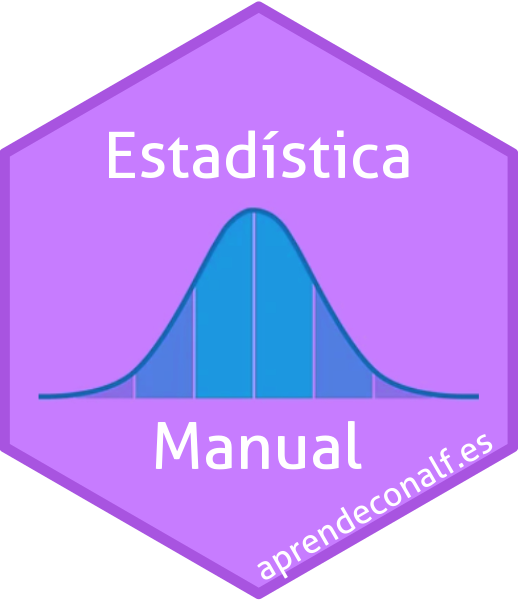
\includegraphics[width=0.4\textwidth]{img/logos/sticker.png}
\end{center}

\vfill

\begin{flushleft}
\begin{tabular}{ll}

\includegraphics[width=0.1\textwidth]{img/logos/aprendeconalf.png} & \parbox[b]{5cm}{\Large\textsf{Alfredo
Sánchez
Alberca}\\ \textsf{asalber@ceu.es} \\ \textsf{https://aprendeconalf.es}}
\end{tabular}
\end{flushleft}
\end{titlepage}\ifdefined\Shaded\renewenvironment{Shaded}{\begin{tcolorbox}[boxrule=0pt, enhanced, sharp corners, breakable, frame hidden, interior hidden, borderline west={3pt}{0pt}{shadecolor}]}{\end{tcolorbox}}\fi

\renewcommand*\contentsname{Indice de contenidos}
{
\hypersetup{linkcolor=}
\setcounter{tocdepth}{2}
\tableofcontents
}
\bookmarksetup{startatroot}

\hypertarget{prefacio}{%
\chapter*{Prefacio}\label{prefacio}}
\addcontentsline{toc}{chapter}{Prefacio}

\markboth{Prefacio}{Prefacio}

¡Bienvenida/os al manual de Estadística!

Este libro es una introducción a la Estadística básica y el cálculo de
probabilidades para alumnos de grados de ciencias e ingenierías.

Este libro se complementa con los siguientes recursos:

\begin{itemize}
\tightlist
\item
  \href{https://aprendeconalf.es/estadistica-ejercicios/}{Colección de
  problemas resueltos}
\item
  \href{https://aprendeconalf.es/estadistica-practicas-r/}{Prácticas de
  Estadística con R}
\end{itemize}

\hypertarget{licencia}{%
\section*{Licencia}\label{licencia}}
\addcontentsline{toc}{section}{Licencia}

\markright{Licencia}

Esta obra está bajo una licencia Reconocimiento -- No comercial --
Compartir bajo la misma licencia 3.0 España de Creative Commons. Para
ver una copia de esta licencia, visite
\url{https://creativecommons.org/licenses/by-nc-sa/3.0/es/}.

Con esta licencia eres libre de:

\begin{itemize}
\tightlist
\item
  Copiar, distribuir y mostrar este trabajo.
\item
  Realizar modificaciones de este trabajo.
\end{itemize}

Bajo las siguientes condiciones:

\begin{itemize}
\item
  **Reconocimiento Debe reconocer los créditos de la obra de la manera
  especificada por el autor o el licenciador (pero no de una manera que
  sugiera que tiene su apoyo o apoyan el uso que hace de su obra).
\item
  **No comercial No puede utilizar esta obra para fines comerciales.
\item
  **Compartir bajo la misma licencia Si altera o transforma esta obra, o
  genera una obra derivada, sólo puede distribuir la obra generada bajo
  una licencia idéntica a ésta.
\end{itemize}

Al reutilizar o distribuir la obra, tiene que dejar bien claro los
términos de la licencia de esta obra.

Estas condiciones pueden no aplicarse si se obtiene el permiso del
titular de los derechos de autor.

Nada en esta licencia menoscaba o restringe los derechos morales del
autor.

\bookmarksetup{startatroot}

\hypertarget{introducciuxf3n-a-la-estaduxedstica}{%
\chapter{Introducción a la
Estadística}\label{introducciuxf3n-a-la-estaduxedstica}}

\hypertarget{quuxe9-es-la-estaduxedstica}{%
\subsection{¿Qué es la estadística?}\label{quuxe9-es-la-estaduxedstica}}

\leavevmode\vadjust pre{\hypertarget{def-estadistica}{}}%
\begin{definition}[Estadística]\label{def-estadistica}

La \emph{estadística} es una rama de las matemáticas que se encarga de
la recogida, análisis e interpretación de datos.

\end{definition}

El papel de la Estadística es extraer información de los datos para
adquirir el conocimiento necesario para tomar decisiones.

\begin{figure}

{\centering 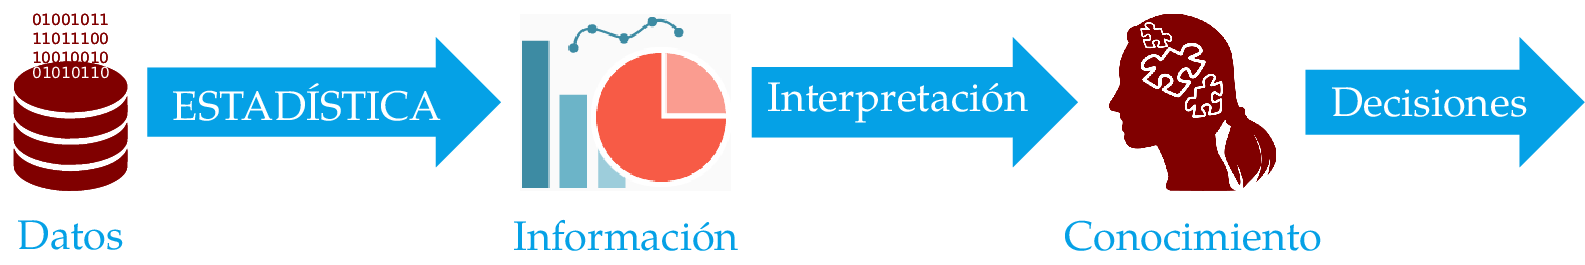
\includegraphics{./img/introduccion/proposito_estadistica.png}

}

\caption{Propósito de la Estadística}

\end{figure}

La estadística es imprescindible en cualquier disciplina científica o
técnica donde se manejen datos, especialmente si son grandes volúmenes
de datos, como por ejemplo en Física, Química, Medicina, Psicología,
Economía o Ciencias Sociales.

Pero, \emph{¿por qué es necesaria la Estadística?}

\hypertarget{la-variabilidad-de-nuestro-mundo}{%
\subsection{La variabilidad de nuestro
mundo}\label{la-variabilidad-de-nuestro-mundo}}

El científico trata de estudiar el mundo que le rodea; un mundo que está
lleno de variaciones que dificultan la determinación del comportamiento
de las cosas.

La estadística actúa como disciplina puente entre la realidad del mundo
y los modelos matemáticos que tratan de explicarla, proporcionando una
metodología para evaluar las discrepancias entre la realidad y los
modelos teóricos.

Esto la convierte en una herramienta indispensable en las ciencias
aplicadas que requieran el análisis de datos y el diseño de
experimentos.

\hypertarget{poblaciuxf3n-y-muestra}{%
\section{Población y muestra}\label{poblaciuxf3n-y-muestra}}

\hypertarget{poblaciuxf3n-estaduxedstica}{%
\subsection{Población estadística}\label{poblaciuxf3n-estaduxedstica}}

\leavevmode\vadjust pre{\hypertarget{def-poblacion}{}}%
\begin{definition}[Población]\label{def-poblacion}

Una \emph{población} es un conjunto de elementos definido por una o más
características que tienen todos los elementos, y sólo ellos. Cada
elemento de la población se llama \emph{individuo}.

\end{definition}

\leavevmode\vadjust pre{\hypertarget{def-tamauxf1o-poblacional}{}}%
\begin{definition}[Tamaño poblacional]\label{def-tamaño-poblacional}

El número de individuos de una población se conoce como \emph{tamaño
poblacional} y se representa como \(N\).

\end{definition}

\leavevmode\vadjust pre{\hypertarget{exm-tamauxf1o-poblacional}{}}%
\begin{example}[]\label{exm-tamaño-poblacional}

En unas elecciones generales a la presidencia del gobierno, la población
serían todos los individuos del estado con derecho a voto. En el estudio
de una enfermedad, la población sería todas las personas que tienen la
enfermedad. Y en un proceso de control de calidad en la fabricación de
un fármaco, la población estaría formada por todos los fármacos que se
producen en la fábrica.

\end{example}

A veces, no todos los elementos de la población están accesibles para su
estudio. Entonces se distingue entre:

\begin{itemize}
\tightlist
\item
  \textbf{Población Teórica}: Conjunto de elementos a los que se quiere
  extrapolar los resultados del estudio.
\item
  \textbf{Población Estudiada}: Conjunto de elementos realmente
  accesibles en el estudio.
\end{itemize}

\leavevmode\vadjust pre{\hypertarget{exm-poblacion-teorica-observada}{}}%
\begin{example}[]\label{exm-poblacion-teorica-observada}

En el caso del estudio de una enfermedad, la población teórica sería
todas las personas que contraigan la enfermedad, incluso si aún no han
nacido, mientras que la población estudiada se limitaría al número de
personas enfermas que realmente podemos estudiar (obsérvese que incluso
quedarían fuera las personas enfermas pero de las que no podemos
conseguir información).

\end{example}

\hypertarget{inconvenientes-en-el-estudio-de-la-poblaciuxf3n}{%
\subsection{Inconvenientes en el estudio de la
población}\label{inconvenientes-en-el-estudio-de-la-poblaciuxf3n}}

El científico estudia un determinado fenómeno en una población para
comprenderlo, obtener conocimiento sobre el mismo, y así poder
controlarlo. Pero, para tener un conocimiento completo de la población
\emph{es necesario estudiar todos los individuos de la misma}. Sin
embargo, esto no siempre es posible por distintos motivos:

\begin{itemize}
\tightlist
\item
  El tamaño de la población es infinito, o bien es finito pero demasiado
  grande.
\item
  Las pruebas a que se someten los individuos son destructivas.
\item
  El coste, tanto de dinero como de tiempo, que supondría estudiar a
  todos los individuos es excesivo.
\end{itemize}

\hypertarget{muestra-estaduxedstica}{%
\subsection{Muestra estadística}\label{muestra-estaduxedstica}}

Cuando no es posible o conveniente estudiar todos los individuos de la
población, se estudia sólo una parte de la misma.

\leavevmode\vadjust pre{\hypertarget{def-muestra}{}}%
\begin{definition}[Muestra]\label{def-muestra}

Una \emph{muestra} es un subconjunto de la población.

\end{definition}

\leavevmode\vadjust pre{\hypertarget{def-tamauxf1o-muestral}{}}%
\begin{definition}[Tamaño muestral]\label{def-tamaño-muestral}

Al número de individuos que componen la muestra se le llama \emph{tamaño
muestral} y se representa por \(n\).

\end{definition}

Habitualmente, el estudio de una población se realiza a partir de
muestras extraídas de dicha población.

Generalmente, el estudio de la muestra sólo aporta conocimiento
aproximado de la población. Pero en muchos casos es \emph{suficiente}.

\hypertarget{determinaciuxf3n-del-tamauxf1o-muestral}{%
\subsection{Determinación del tamaño
muestral}\label{determinaciuxf3n-del-tamauxf1o-muestral}}

Una de las preguntas más interesantes que surge inmediatamente es:
\emph{¿cuántos individuos es necesario tomar en la muestra para tener un
conocimiento aproximado pero suficiente de la población?}

La respuesta depende de varios factores, como la variabilidad de la
población o la fiabilidad deseada para las extrapolaciones que se hagan
hacia la población.

Por desgracia no se podrá responder hasta casi el final del curso, pero
en general, cuantos más individuos haya en la muestra, más fiables serán
las conclusiones sobre la población, pero también será más lento y
costoso el estudio.

\leavevmode\vadjust pre{\hypertarget{exm-tamauxf1o-muestral-suficiente}{}}%
\begin{example}[]\label{exm-tamaño-muestral-suficiente}

Para entender a qué nos referimos cuando hablamos de un tamaño muestral
suficiente para comprender lo que ocurre en la población, podemos
utilizar el siguiente símil en que se trata de comprender el motivo que
representa una fotografía.

Una fotografía digital está formada por multitud de pequeños puntitos
llamados pixels que se dispone en una enorme tabla de filas y columnas
(cuantas más filas y columnas haya se habla de que la foto tiene más
resolución). Aquí la población estaría formada por todos y cada uno de
los píxeles que forman la foto. Por otro lado cada pixel tiene un color
y es la variedad de colores a lo largo de los pixels la que permite
formar la imagen de la fotografía.

\emph{¿Cuántos píxeles debemos tomar en una muestra para averiguar la
imagen de la foto?}

La respuesta depende de la variabilidad de colores en la foto. Si todos
los pixels de la foto son del mismo color, entonces un sólo pixel basta
para desvelar la imagen. Pero, si la foto tiene mucha variabilidad de
colores, necesitaremos muchos más pixels en la muestra para descubrir el
motivo de la foto.

La imagen siguiente contiene una muestra pequeña de píxeles de una foto.
¿Puedes averiguar el motivo de a foto?

\begin{figure}

{\centering 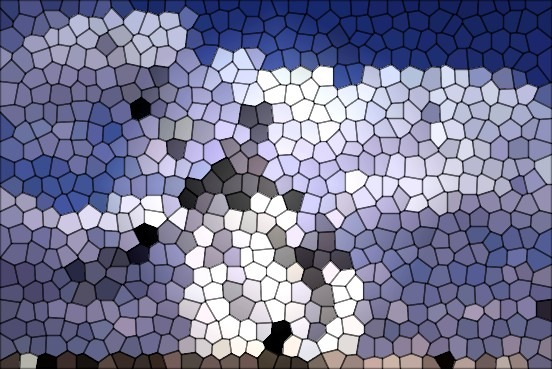
\includegraphics{./img/introduccion/muestra_molinos1.jpg}

}

\caption{Muestra pequeña de píxeles de una foto.}

\end{figure}

\emph{¡Con una muestra pequeña es difícil averiguar el contenido de la
imagen!}

Seguramente no has podido averiguar el motivo de la fotografía, porque
en este caso el número de píxeles que hemos tomado en la muestra es
insuficiente para comprender toda la variabilidad de colores que hay en
la foto.

La siguiente imagen contiene una muestra mayor de píxeles. ¿Eres capaz
de adivinar el motivo de la foto ahora?

\begin{figure}

{\centering 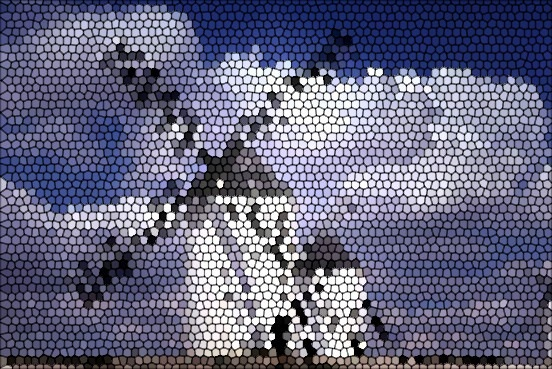
\includegraphics{./img/introduccion/muestra_molinos2.jpg}

}

\caption{Muestra mayor de píxeles de una foto.}

\end{figure}

\emph{¡Con una muestra mayor es posible desvelar el motivo de la foto!}

Y aquí está la población completa.

\begin{figure}

{\centering 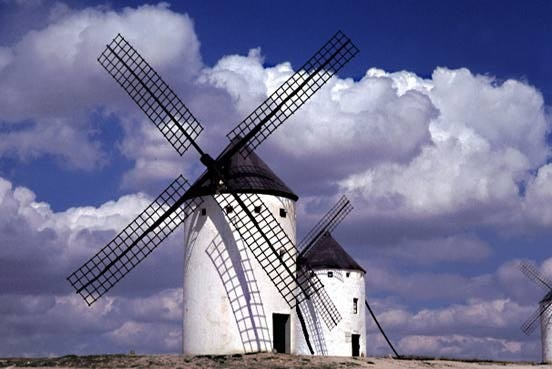
\includegraphics{./img/introduccion/muestra_molinos3.jpg}

}

\caption{Población de píxeles de una foto.}

\end{figure}

Lo importante es que \emph{¡No es necesario conocer todos los píxeles
para averiguar la imagen!}

\end{example}

\hypertarget{tipos-de-razonamiento}{%
\subsection{Tipos de razonamiento}\label{tipos-de-razonamiento}}

Así pues, habitualmente realizaremos el estudio de la población a partir
de muestras y luego trataremos de extrapolar lo observado en la muestra
al resto de la población. A este tipo de razonamiento que saca
conclusiones desde la muestra hacia la población se le conoce como
\emph{razonamiento inductivo}.

\begin{figure}

{\centering 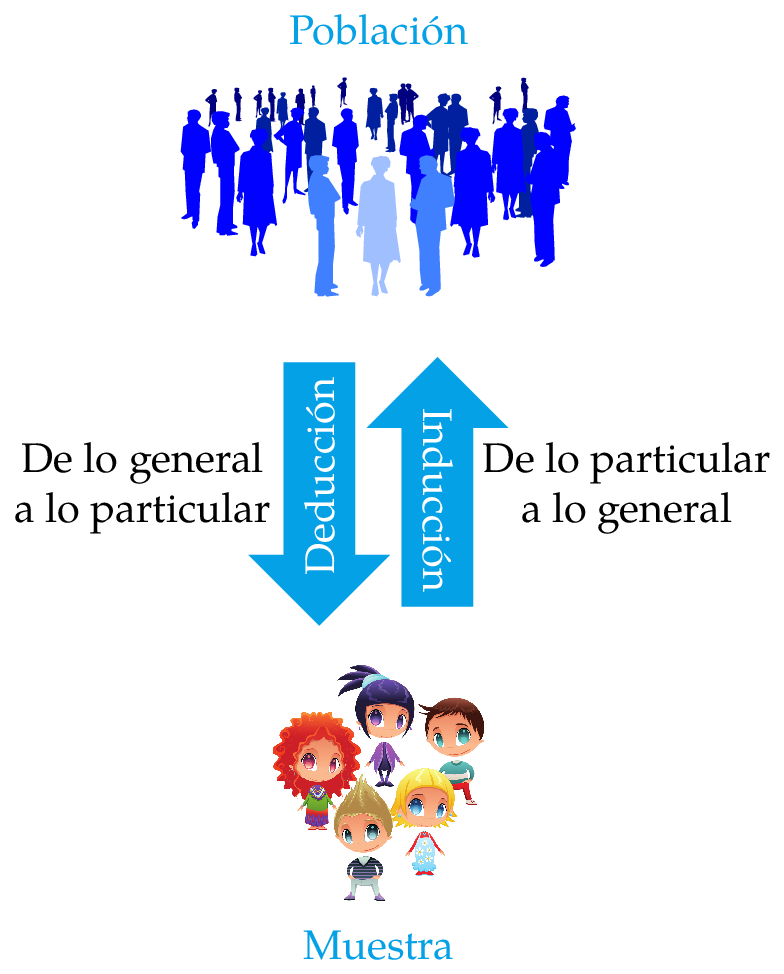
\includegraphics{./img/introduccion/tipos_razonamiento.png}

}

\caption{Tipos de razonamiento.}

\end{figure}

\begin{itemize}
\item
  \emph{Características de la deducción}: Si las premisas son ciertas,
  garantiza la certeza de las conclusiones (es decir, si algo se cumple
  en la población, también se cumple en la muestra). Sin embargo,
  \emph{¡no aporta conocimiento nuevo!}
\item
  \emph{Características de la inducción}: No garantiza la certeza de las
  conclusiones (si algo se cumple en la muestra, puede que no se cumpla
  en la población, así que ¡cuidado con las extrapolaciones!), pero
  \emph{¡es la única forma de generar conocimiento nuevo!}
\end{itemize}

La estadística se apoya fundamentalmente en el razonamiento inductivo ya
que utiliza la información obtenida a partir de muestras para sacar
conclusiones sobre las poblaciones. A diferencia del razonamiento
deductivo que va de lo general a lo particular, o en nuestro caso de la
población a la muestra, el razonamiento inductivo no garantiza la
certeza de las conclusiones, por lo que debemos ser cuidadosos a la hora
de generalizar sobre la población lo observado en al muestra, ya que si
la muestra no es representativa de la población o contiene sesgos, las
conclusiones pueden ser erróneas.

\hypertarget{muestreo}{%
\section{Muestreo}\label{muestreo}}

\leavevmode\vadjust pre{\hypertarget{def-muestreo}{}}%
\begin{definition}[Muestreo]\label{def-muestreo}

El proceso de selección de los elementos que compondrán una muestra se
conoce como \emph{muestreo}.

\end{definition}

{[}{]}(img/introduccion/muestreo.svg'' alt=``Muestreo''
width=``500px''\textgreater{}

Para que una muestra refleje información fidedigna sobre la población
global debe ser representativa de la misma, lo que significa que debe
reproducir a pequeña escala la variabilidad de la población.

\emph{El objetivo es obtener una muestra representativa de la
población.}

\hypertarget{modalidades-de-muestreo}{%
\subsection{Modalidades de muestreo}\label{modalidades-de-muestreo}}

Existen muchas técnicas de muestreo pero se pueden agrupar en dos
categorías:

\begin{itemize}
\item
  \textbf{Muestreo Aleatorio}: Elección aleatoria de los individuos de
  la muestra. Todos tienen la misma probabilidad de ser elegidos
  (\emph{equiprobabilidad}).
\item
  \textbf{Muestreo No Aleatorio}: Los individuos se eligen de forma no
  aleatoria. Algunos individuos tienen más probabilidad de ser
  seleccionados que otros.
\end{itemize}

Sólo las técnicas aleatorias evitan el sesgo de selección, y por tanto,
garantizan la representatividad de la muestra extraída, y en
consecuencia la validez de las conclusiones.

Las técnicas no aleatorias no sirven para hacer generalizaciones, ya que
no garantizan la representatividad de la muestra. Sin embargo, son menos
costosas y pueden utilizarse en estudios exploratorios.

\hypertarget{muestreo-aleatorio-simple}{%
\subsection{Muestreo aleatorio simple}\label{muestreo-aleatorio-simple}}

Dentro de las modalidades de muestreo aleatorio, el tipo más conocido es
el \emph{muestreo aleatorio simple}, caracterizado por:

\begin{itemize}
\tightlist
\item
  Todos los individuos de la población tienen la misma probabilidad de
  ser elegidos para la muestra.
\item
  La selección de individuos es con reemplazamiento, es decir, cada
  individuo seleccionado es devuelto a la población antes de seleccionar
  al siguiente (y por tanto no se altera la población de partida).
\item
  Las sucesivas selecciones de un individuo son independientes.
\end{itemize}

La única forma de realizar un muestreo aleatorio es asignar un número a
cada individuo de la población (\emph{censo}) y realizar un sorteo
aleatorio.

\hypertarget{variables-estaduxedsticas}{%
\subsection{Variables estadísticas}\label{variables-estaduxedsticas}}

Todo estudio estadístico comienza por la identificación de las
características que interesa estudiar en la población y que se medirán
en los individuos de la muestra.

\leavevmode\vadjust pre{\hypertarget{def-variable-estadistica}{}}%
\begin{definition}[Variable estadística]\label{def-variable-estadistica}

Una \emph{variable estadística} es una propiedad o característica medida
en los individuos de la población.

Los \emph{datos} son los valores observados en las variables
estadísticas.

\end{definition}

\begin{figure}

{\centering 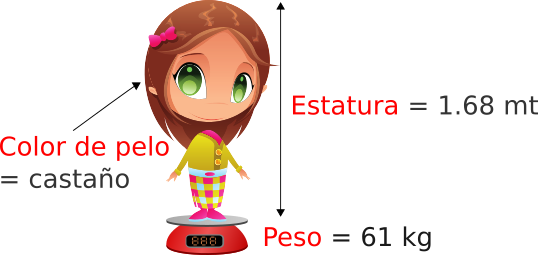
\includegraphics{./img/introduccion/variables_estadisticas.png}

}

\caption{Variables estadísticas.}

\end{figure}

Estas características pueden ser de distintos tipos de acuerdo a su
naturaleza y su escala:

\begin{itemize}
\item
  \textbf{Variables cualitativas o atributos}: Miden cualidades no
  numéricas. Pueden ser:

  \begin{itemize}
  \item
    \textbf{Nominales}: No existe un orden entre las categorías.\\
    Ejemplo: El color de pelo o el sexo.
  \item
    \textbf{Ordinales}: Existe un orden entre las categorías. Ejemplo:
    El nivel de estudios o la gravedad de una enfermedad.
  \end{itemize}
\item
  \textbf{Variables cuantitativas}: Miden cantidades numéricas. Pueden
  ser:

  \begin{itemize}
  \item
    \textbf{Discretas}: Toman valores numéricos aislados (habitualmente
    números enteros).\\
    Ejemplo: El número de hijos o el número de coches en una familia.
  \item
    \textbf{Continuas}: Pueden tomar cualquier valor en un intervalo
    real.\\
    Ejemplo: El peso o la estatura.
  \end{itemize}
\end{itemize}

Las variables cualitativas y discretas se conocen también con
\emph{variables categóricas} y sus valores \emph{categorías}.

\begin{figure}

{\centering 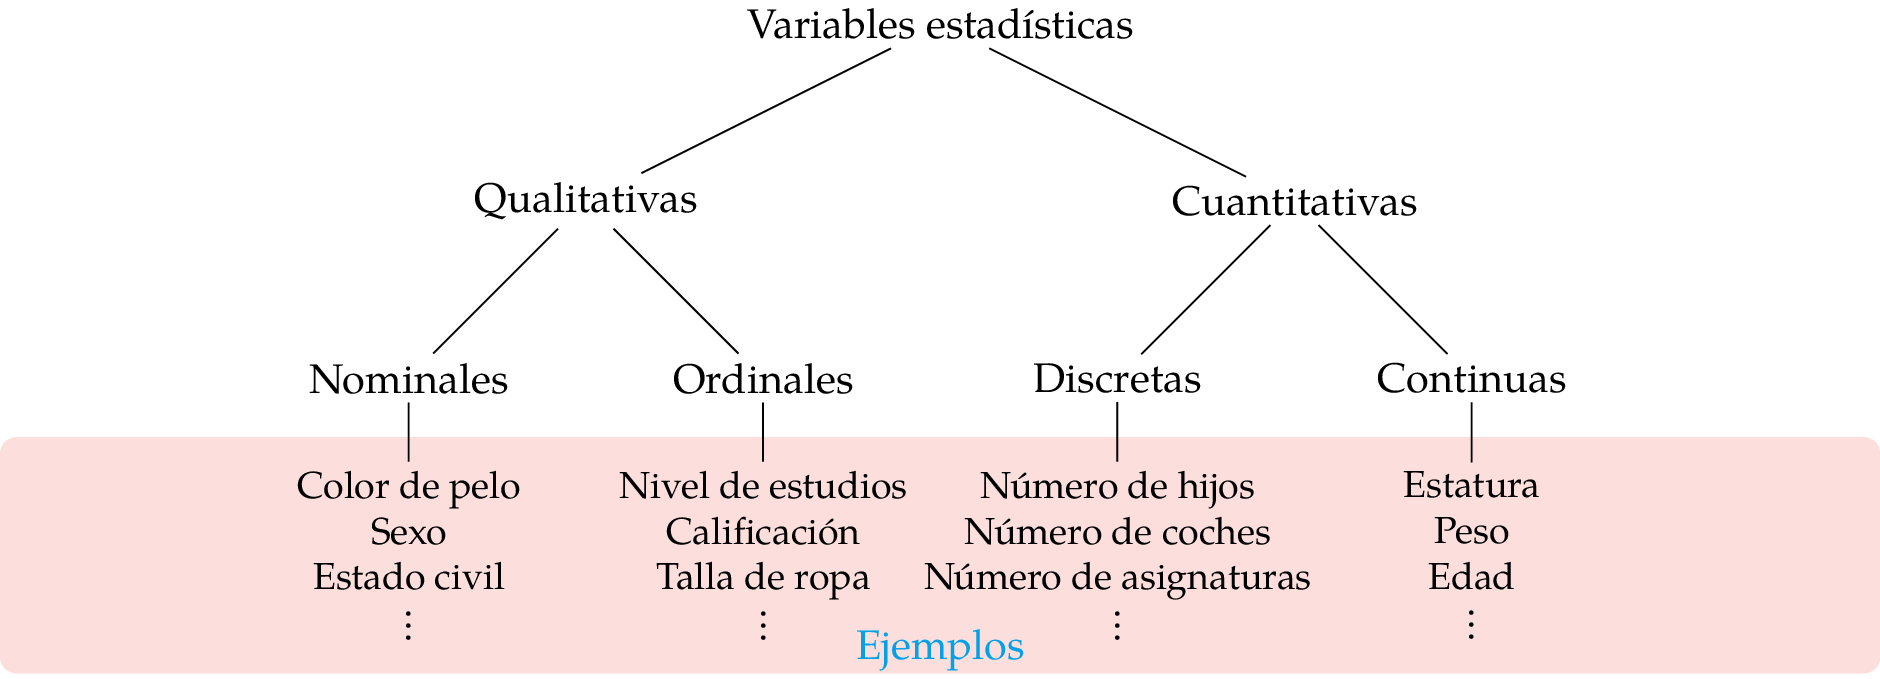
\includegraphics{./img/introduccion/tipos_variables.png}

}

\caption{Tipos de variables estadísticas.}

\end{figure}

\hypertarget{elecciuxf3n-del-tipo-de-variable-muxe1s-apropiado}{%
\subsubsection{Elección del tipo de variable más
apropiado}\label{elecciuxf3n-del-tipo-de-variable-muxe1s-apropiado}}

En ocasiones una característica puede medirse mediante variables de
distinto tipo.

\leavevmode\vadjust pre{\hypertarget{exm-eleccion-tipos-variables}{}}%
\begin{example}[]\label{exm-eleccion-tipos-variables}

Si una persona fuma o no podría medirse de diferentes formas:

\begin{itemize}
\item
  Fuma: si/no. (Nominal)
\item
  Nivel de fumador: No fuma / ocasional / moderado / bastante /
  empedernido. (Ordinal)
\item
  Número de cigarros diarios: 0,1,2,\ldots{} (Discreta)
\end{itemize}

\end{example}

En estos casos es preferible usar variables cuantitativas a
cualitativas. Dentro de las cuantitativas es preferible usar las
continuas a las discretas y dentro de las cualitativas es preferible
usar ordinales a nominales pues aportan más información.

\begin{figure}

{\centering 
\includegraphics{./img/introduccion/informacion_variables.png}

}

\caption{Cantidad de información de los tipos de variables
estadísticas.}

\end{figure}

De acuerdo al papel que juegan en el estudio las variables también
pueden clasificarse como:

\begin{itemize}
\item
  \textbf{Variables independientes}: Variables que supuestamente no
  dependen de otras variables en el estudio. Habitualmente son las
  variables manipuladas en el experimento para ver su efecto en las
  variables dependientes. Se conocen también como \emph{variables
  predictivas}.
\item
  \textbf{Variables dependientes}: Variables que supuestamente dependen
  de otras variables en el estudio. No son manipuladas en el experimento
  y también se conocen como \emph{variables respuesta}.
\end{itemize}

\leavevmode\vadjust pre{\hypertarget{exm-variables-dependientes-independientes}{}}%
\begin{example}[]\label{exm-variables-dependientes-independientes}

En un estudio sobre el rendimiento de los alumnos de un curso, la
inteligencia de los alumnos y el número de horas de estudio diarias
serían variables independientes y la nota del curso sería una variable
dependiente.

\end{example}

\hypertarget{tipos-de-estudios-estaduxedsticos}{%
\subsection{Tipos de estudios
estadísticos}\label{tipos-de-estudios-estaduxedsticos}}

Dependiendo de si se manipulan las variables independientes existen dos
tipos de estudios:

\begin{itemize}
\tightlist
\item
  \textbf{Experimentales}: Cuando las variables independientes son
  manipuladas para ver el efecto que producen en las variables
  dependientes.
\end{itemize}

\leavevmode\vadjust pre{\hypertarget{exm-estudios-experimentales}{}}%
\begin{example}[]\label{exm-estudios-experimentales}

En un estudio sobre el rendimiento de los estudiantes en un test, el
profesor manipula la metodología de estudio para crear dos o más grupos
con metodologías de estudio distintas.

\end{example}

\begin{itemize}
\tightlist
\item
  \textbf{No experimentales}: Cuando las variables independientes no son
  manipuladas. Esto no significa que sea imposible hacerlo, sino que es
  difícil o poco ético hacerlo.
\end{itemize}

\leavevmode\vadjust pre{\hypertarget{exm-estudios-no-experimentales}{}}%
\begin{example}[]\label{exm-estudios-no-experimentales}

En un estudio un investigador puede estar interesado en el efecto de
fumar sobre el cáncer de pulmón. Aunque es posible, no sería ético
pedirle a los pacientes que fumasen para ver el efecto que tiene sobre
sus pulmones. En este caso, el investigador podría estudiar dos grupos
de pacientes, uno con cáncer de pulmón y otro sin cáncer, y observar en
cada grupo cuántos fuman o no.

\end{example}

Los estudios experimentales permiten identificar causas y efectos entre
las variables del estudio, mientras que los no experimentales sólo
permiten identificar relaciones de asociación entre las variables.

\hypertarget{la-tabla-de-datos}{%
\subsection{La tabla de datos}\label{la-tabla-de-datos}}

Las variables a estudiar se medirán en cada uno de los individuos de la
muestra, obteniendo un conjunto de datos que suele organizarse en forma
de matriz que se conoce como tabla de datos\_.

En esta tabla cada columna contiene la información de una variable y
cada fila la información de un individuo.

\leavevmode\vadjust pre{\hypertarget{exm-tabla-datos}{}}%
\begin{example}[]\label{exm-tabla-datos}

La siguiente tabla contiene información de las variables Nombre, Edad,
Sexo, Peso y Altura de una muestra de 6 personas.

\begin{longtable}[]{@{}lcccc@{}}
\toprule()
Nombre & Edad & Sexo & Peso(Kg) & Altura(cm) \\
\midrule()
\endhead
José Luis Martínez & 18 & H & 85 & 179 \\
Rosa Díaz & 32 & M & 65 & 173 \\
Javier García & 24 & H & 71 & 181 \\
Carmen López & 35 & M & 65 & 170 \\
Marisa López & 46 & M & 51 & 158 \\
Antonio Ruiz & 68 & H & 66 & 174 \\
\bottomrule()
\end{longtable}

\end{example}

\hypertarget{fases-del-anuxe1lisis-estaduxedstico}{%
\subsection{Fases del análisis
estadístico}\label{fases-del-anuxe1lisis-estaduxedstico}}

Normalmente un estudio estadístico pasa por las siguientes etapas:

\begin{enumerate}
\def\labelenumi{\arabic{enumi}.}
\item
  El estudio comienza por el diseño previo del mismo en el que se
  establezcan los objetivos del mismo, la población, las variables que
  se medirán y el tamaño muestral requerido.
\item
  A continuación se seleccionará una muestra representativa del tamaño
  establecido y se medirán las variables en los individuos de la muestra
  obteniendo la tabla de datos. De esto se encarga el \emph{Muestreo}.
\item
  El siguiente paso consiste en describir y resumir la información que
  contiene la muestra. De esto se encarga la \emph{Estadística
  Descriptiva}.
\item
  La información obtenida es proyectada sobre un modelo matemático que
  intenta explicar el comportamiento de la población y el modelo se
  valida. De todo esto se encarga la \emph{Estadística Inferencial}.
\item
  Finalmente, el modelo validado nos permite hacer predicciones y sacar
  conclusiones sobre la población de partida con cierta confianza.
\end{enumerate}

\hypertarget{el-ciclo-estaduxedstico}{%
\subsubsection{El ciclo estadístico}\label{el-ciclo-estaduxedstico}}

\begin{figure}

{\centering 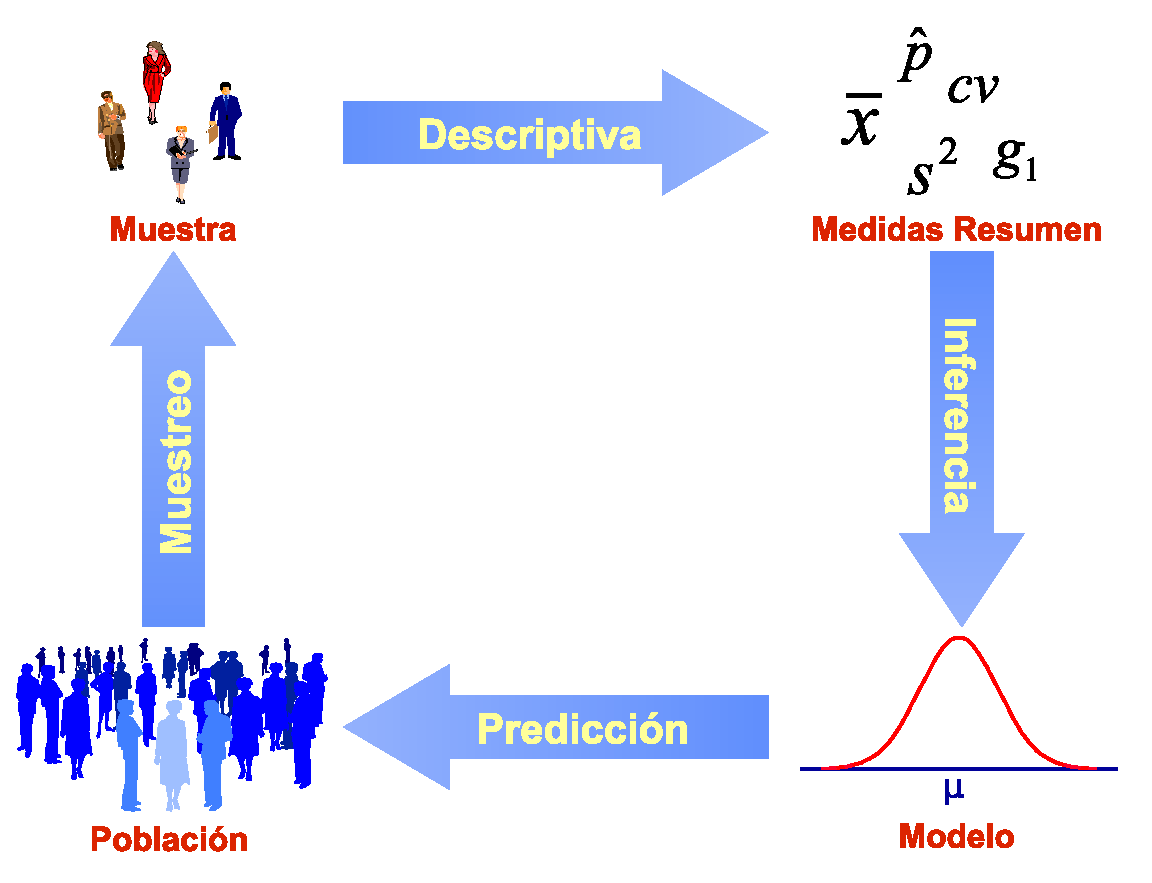
\includegraphics{./img/introduccion/ciclo_estadistico.eps}

}

\caption{El ciclo estadístico.}

\end{figure}

\bookmarksetup{startatroot}

\hypertarget{estaduxedstica-descriptiva}{%
\chapter{Estadística Descriptiva}\label{estaduxedstica-descriptiva}}

La estadística descriptiva es la parte de la estadística encargada de
representar, analizar y resumir la información contenida en la muestra.

Tras el proceso de muestreo, es la siguiente etapa de todo estudio
estadístico y suele consistir en:

\begin{enumerate}
\def\labelenumi{\arabic{enumi}.}
\item
  Clasificar, agrupar y ordenar los datos de la muestra.
\item
  Tabular y representar gráficamente los datos de acuerdo a sus
  frecuencias.
\item
  Calcular medidas que resuman la información que contiene la muestra
  (\emph{estadísticos muestrales}).
\end{enumerate}

\begin{tcolorbox}[enhanced jigsaw, coltitle=black, breakable, bottomrule=.15mm, colback=white, bottomtitle=1mm, toprule=.15mm, opacitybacktitle=0.6, titlerule=0mm, toptitle=1mm, title=\textcolor{quarto-callout-important-color}{\faExclamation}\hspace{0.5em}{Importante}, colframe=quarto-callout-important-color-frame, opacityback=0, arc=.35mm, left=2mm, rightrule=.15mm, leftrule=.75mm, colbacktitle=quarto-callout-important-color!10!white]

No tiene poder inferencial, por lo que nunca deben sacarse conclusiones
sobre la población a partir de las medidas resumen que aporta la
Estadística Descriptiva.

\end{tcolorbox}

El estudio de una variable estadística comienza por medir la variable en
los individuos de la muestra y clasificar los valores obtenidos.

Existen dos formas de clasificar estos valores:

\begin{itemize}
\item
  \textbf{Sin agrupar}: Ordenar todos los valores obtenidos en la
  muestra de menor a mayor. Se utiliza con atributos y variables
  discretas con pocos valores diferentes.
\item
  \textbf{Agrupados}: Agrupar los valores en clases (intervalos) y
  ordenar dichas clases de menor a mayor. Se utiliza con variables
  continuas y con variables discretas con muchos valores diferentes.
\end{itemize}

\hypertarget{clasificaciuxf3n-de-la-muestra}{%
\subsection{Clasificación de la
muestra}\label{clasificaciuxf3n-de-la-muestra}}

Consiste colocar juntos los valores iguales y ordenarlos si existe un
orden entre ellos.

\begin{figure}

{\centering 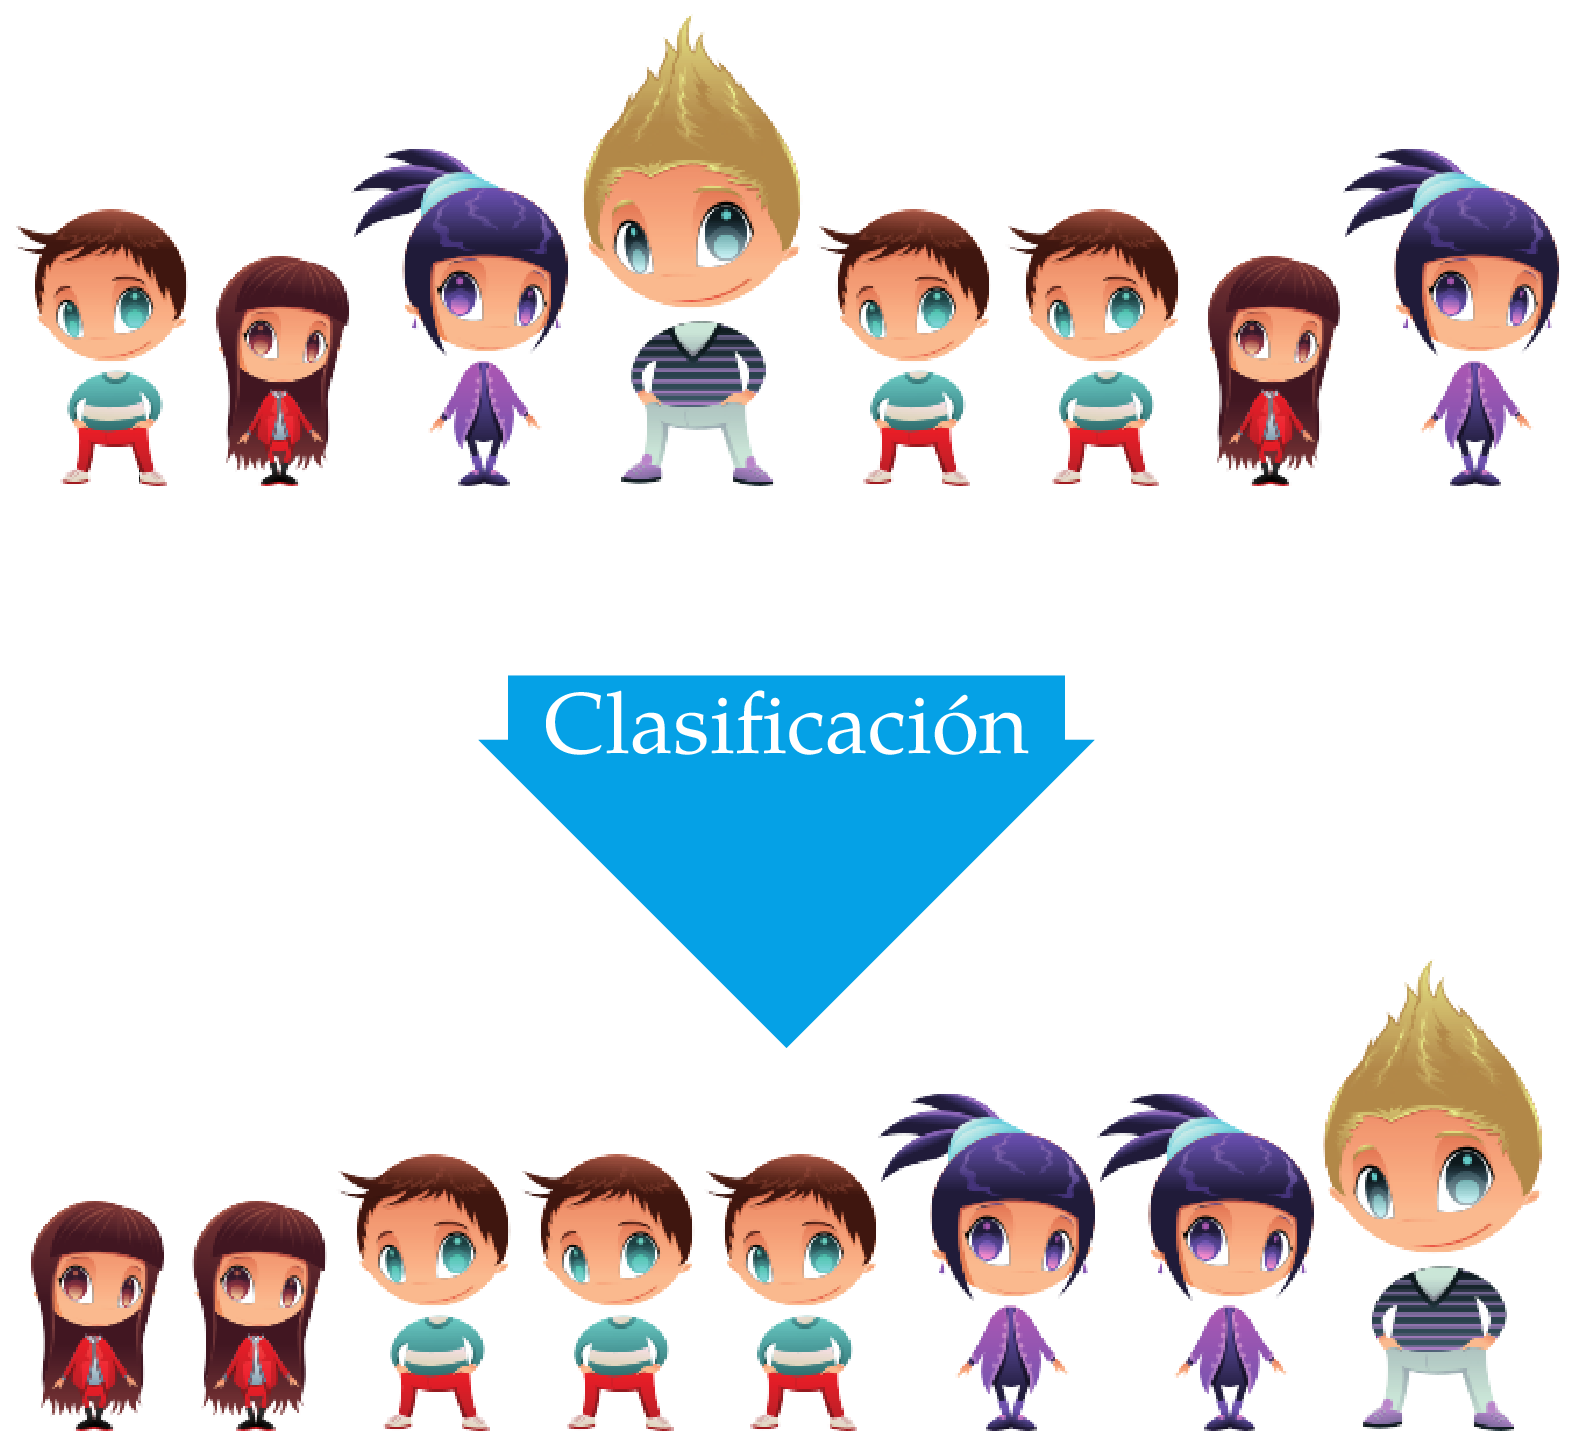
\includegraphics{./img/descriptiva/clasificacion_muestra.png}

}

\caption{Clasificación de la muestra.}

\end{figure}

\hypertarget{recuento-de-frecuencias}{%
\subsection{Recuento de frecuencias}\label{recuento-de-frecuencias}}

\begin{figure}

{\centering 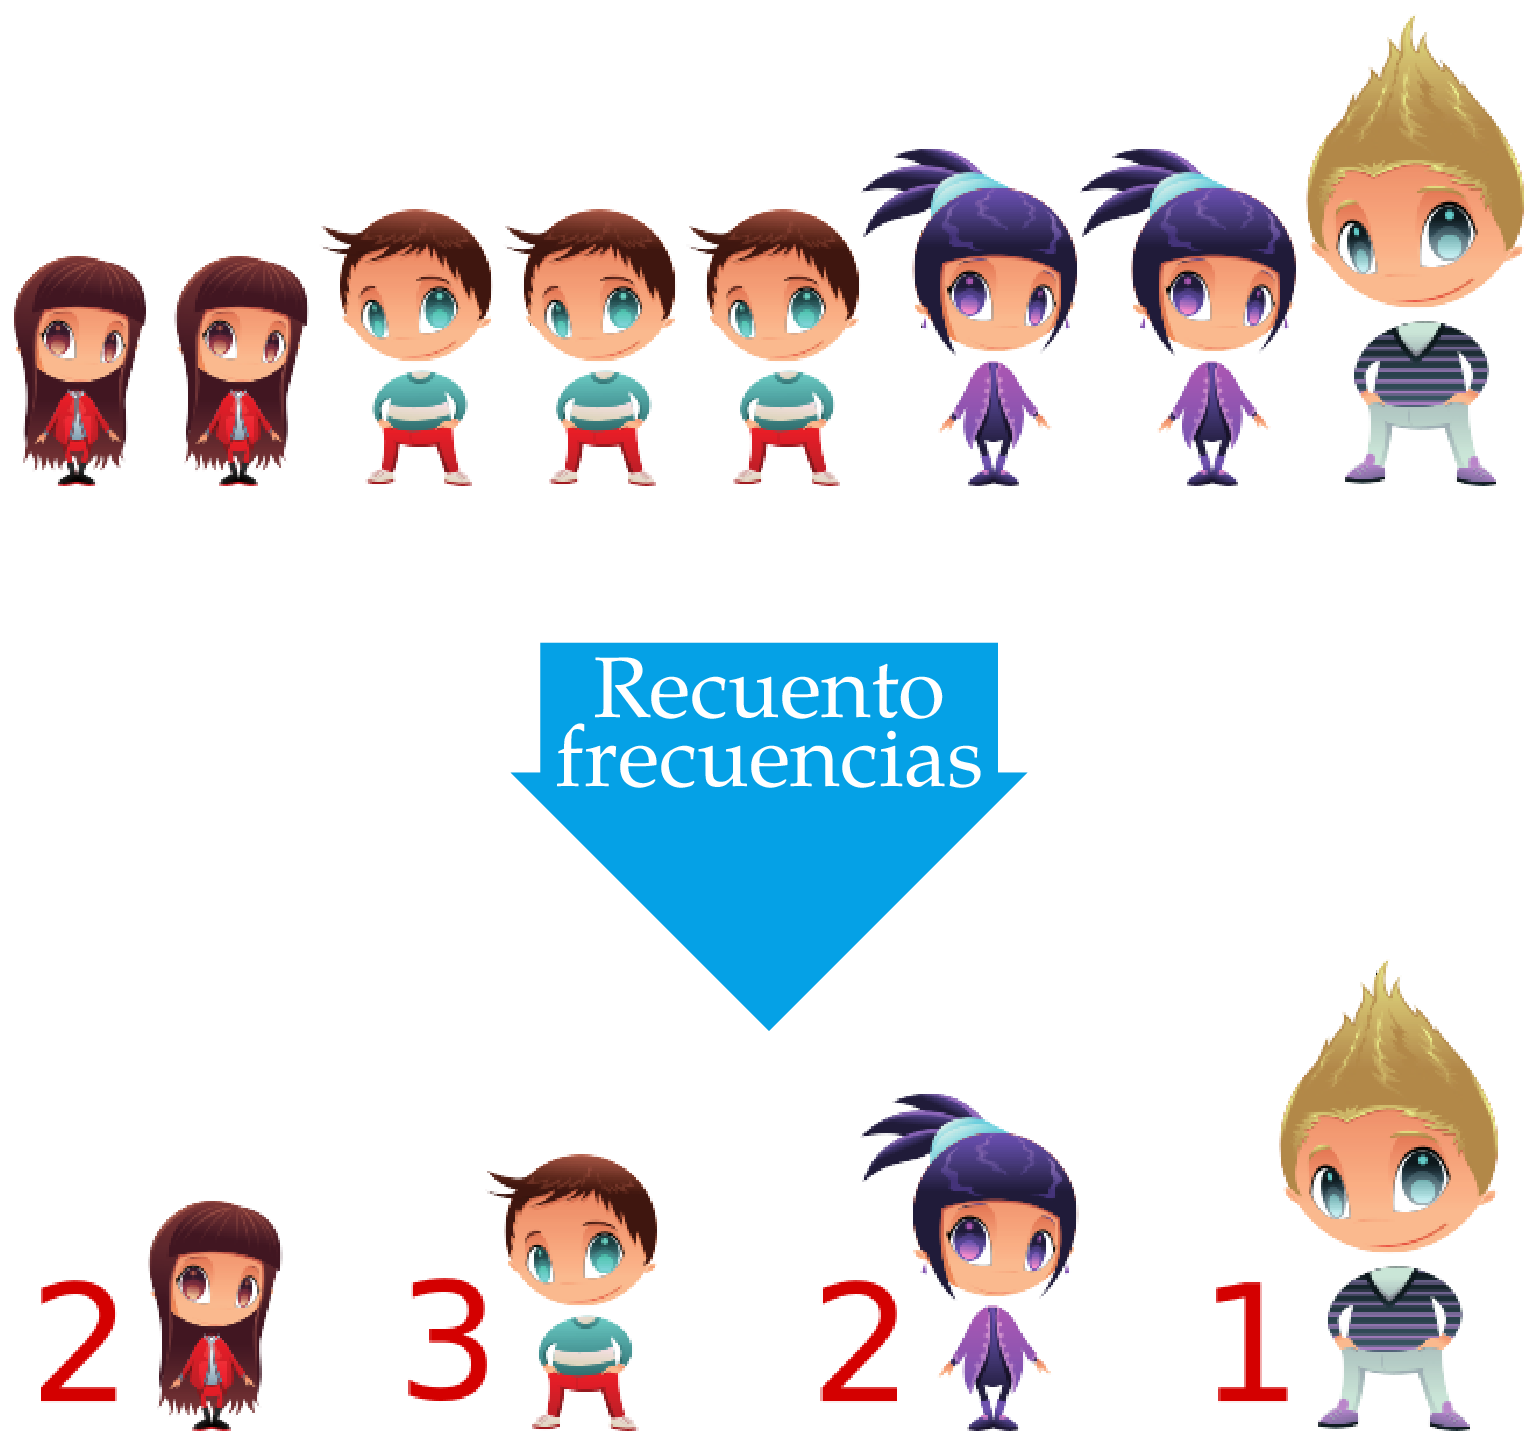
\includegraphics{./img/descriptiva/recuento_frecuencias.png}

}

\caption{Recuento de frecuencias}

\end{figure}

\hypertarget{frecuencias-muestrales}{%
\section{Frecuencias muestrales}\label{frecuencias-muestrales}}

\leavevmode\vadjust pre{\hypertarget{def-frecuencias-muestrales}{}}%
\begin{definition}[Frecuencias
muestrales]\label{def-frecuencias-muestrales}

Dada una muestra de tamaño \(n\) de una variable \(X\), para cada valor
de la variable \(x_i\) observado en la muestra, se define

\begin{itemize}
\tightlist
\item
  \textbf{Frecuencia Absoluta \(n_i\)}: Es el número de veces que el
  valor \(x_i\) aparece en la muestra.
\item
  \textbf{Frecuencia Relativa \(f_i\)}: Es la proporción de veces que el
  valor \(x_i\) aparece en la muestra. \[f_i = \frac{n_i}{n}\]
\item
  \textbf{Frecuencia Absoluta Acumulada \(N_i\)}: Es el número de
  valores en la muestra menores o iguales que \(x_i\).
  \[N_i = n_1 + \cdots + n_i = N_{i-1}+n_i\]
\item
  \textbf{Frecuencia Relativa Acumulada \(F_i\)}: Es la proporción de
  valores en la muestra menores o iguales que \(x_i\).
  \[F_i = \frac{N_i}{n}\]
\end{itemize}

\end{definition}

\hypertarget{tabla-de-frecuencias}{%
\subsection{Tabla de frecuencias}\label{tabla-de-frecuencias}}

Al conjunto de valores observados en la muestra junto a sus respectivas
frecuencias se le denomina \textbf{distribución de frecuencias} y suele
representarse mediante una \textbf{tabla de frecuencias}.

\begin{longtable}[]{@{}
  >{\centering\arraybackslash}p{(\columnwidth - 8\tabcolsep) * \real{0.1273}}
  >{\centering\arraybackslash}p{(\columnwidth - 8\tabcolsep) * \real{0.1727}}
  >{\centering\arraybackslash}p{(\columnwidth - 8\tabcolsep) * \real{0.1727}}
  >{\centering\arraybackslash}p{(\columnwidth - 8\tabcolsep) * \real{0.2636}}
  >{\centering\arraybackslash}p{(\columnwidth - 8\tabcolsep) * \real{0.2636}}@{}}
\toprule()
\begin{minipage}[b]{\linewidth}\centering
Valores de \(X\)
\end{minipage} & \begin{minipage}[b]{\linewidth}\centering
Frecuencia Absoluta
\end{minipage} & \begin{minipage}[b]{\linewidth}\centering
Frecuencia Relativa
\end{minipage} & \begin{minipage}[b]{\linewidth}\centering
Frecuencia Absoluta Acumulada
\end{minipage} & \begin{minipage}[b]{\linewidth}\centering
Frecuencia Relativa Acumulada
\end{minipage} \\
\midrule()
\endhead
\(x_1\) & \(n_1\) & \(f_1\) & \(N_1\) & \(F_1\) \\
\(\vdots\) & \(\vdots\) & \(\vdots\) & \(\vdots\) & \(\vdots\) \\
\(x_i\) & \(n_i\) & \(f_i\) & \(N_i\) & \(F_i\) \\
\(\vdots\) & \(\vdots\) & \(\vdots\) & \(\vdots\) & \(\vdots\) \\
\(x_k\) & \(n_k\) & \(f_k\) & \(N_k\) & \(F_k\) \\
\bottomrule()
\end{longtable}

\leavevmode\vadjust pre{\hypertarget{exm-tabla-frecuencias-datos-no-agrupados}{}}%
\begin{example}[Variable cuantitativa y datos no
agrupados]\label{exm-tabla-frecuencias-datos-no-agrupados}

El número de hijos en 25 familias es:

1, 2, 4, 2, 2, 2, 3, 2, 1, 1, 0, 2, 2, 0, 2, 2, 1, 2, 2, 3, 1, 2, 2, 1,
2

La tabla de frecuencias del número de hijos en esta muestra es

\[ 
\begin{array}{rrrrr}
\hline
x_i & n_i & f_i & N_i & F_i\\
\hline
0 & 2 & 0.08 & 2 & 0.08\\
1 & 6 & 0.24 & 8 & 0.32\\
2 & 14 & 0.56 & 22 & 0.88\\
3 & 2 & 0.08 & 24 & 0.96\\
4 & 1 & 0.04 & 25 & 1 \\
\hline
\sum & 25 & 1 \\
\hline
\end{array}
\]

\end{example}

\leavevmode\vadjust pre{\hypertarget{exm-tabla-frecuencias-datos-agrupados}{}}%
\begin{example}[Variable cuantitativa y datos
agrupados]\label{exm-tabla-frecuencias-datos-agrupados}

Se ha medido la estatura (en cm) de 30 universitarios obteniendo:

179, 173, 181, 170, 158, 174, 172, 166, 194, 185, 162, 187, 198, 177,
178, 165, 154, 188, 166, 171, 175, 182, 167, 169, 172, 186, 172, 176,
168, 187.

La tabla de frecuencias de la estatura en a esta muestra es

\[ 
\begin{array}{crrrr}
\hline
x_i & n_i & f_i & N_i & F_i\\
\hline
(150,160] & 2 & 0.07 & 2 & 0.07\\
(160,170] & 8 & 0.27 & 10 & 0.34\\
(170,180] & 11 & 0.36 & 21 & 0.70\\
(180,190] & 7 & 0.23 & 28 & 0.93\\
(190,200] & 2 & 0.07 & 30 & 1 \\
\hline
\sum & 30 & 1 \\
\hline
\end{array}
\]

\end{example}

\hypertarget{construcciuxf3n-de-clases}{%
\subsection{Construcción de clases}\label{construcciuxf3n-de-clases}}

Cada intervalo de agrupación de datos se denomina \textbf{clase} y el
centro del intervalo se llama \textbf{marca de clase}.

A la hora de agrupar los datos en clases hay que tener en cuenta lo
siguiente:

\begin{itemize}
\tightlist
\item
  El número de intervalos no debe ser muy grande ni muy pequeño. Una
  regla orientativa es tomar un número de intervalos próximo a
  \(\sqrt{n}\) o \(\log_2(n)\).
\item
  Los intervalos no deben solaparse y deben cubrir todo el rango de
  valores. Es indiferente si se abren por la izquierda y se cierran por
  la derecha o al revés.
\item
  El valor más pequeño debe caer dentro del primer intervalo y el más
  grande dentro del último.
\end{itemize}

\leavevmode\vadjust pre{\hypertarget{exm-tabla-frecuencias-cualitativa}{}}%
\begin{example}[Variable
cualitativa]\label{exm-tabla-frecuencias-cualitativa}

Los grupos sanguíneos de una muestra de 30 personas son:

A, B, B, A, AB, 0, 0, A, B, B, A, A, A, A, AB, A, A, A, B, 0, B, B, B,
A, A, A, 0, A, AB, 0.

La tabla de frecuencias del grupo sanguíneo en esta muestra es

\[
\begin{array}{crr}
\hline
x_i & n_i & f_i \\
\hline
\mbox{0} & 5 & 0.16 \\
\mbox{A} & 14 & 0.47 \\
\mbox{B} & 8 & 0.27 \\
\mbox{AB} & 3 & 0.10 \\
\hline
\sum & 30 & 1 \\
\hline
\end{array}
\]

\end{example}

\begin{tcolorbox}[enhanced jigsaw, coltitle=black, breakable, bottomrule=.15mm, colback=white, bottomtitle=1mm, toprule=.15mm, opacitybacktitle=0.6, titlerule=0mm, toptitle=1mm, title=\textcolor{quarto-callout-warning-color}{\faExclamationTriangle}\hspace{0.5em}{Advertencia}, colframe=quarto-callout-warning-color-frame, opacityback=0, arc=.35mm, left=2mm, rightrule=.15mm, leftrule=.75mm, colbacktitle=quarto-callout-warning-color!10!white]

Obsérvese que en este caso las frecuencias acumuladas no tienen sentido
al no existir un orden entre los valores de la variable.

\end{tcolorbox}

\hypertarget{representaciones-gruxe1ficas}{%
\section{Representaciones gráficas}\label{representaciones-gruxe1ficas}}

La tabla de frecuencias también suele representarse gráficamente.
Dependiendo del tipo de variable y de si se han agrupado o no los datos,
se utilizan distintos tipos de gráficos:

\begin{itemize}
\item
  Diagrama de barras
\item
  Histograma
\item
  Diagrama de líneas o polígonos.
\item
  Diagrama de sectores.
\end{itemize}

\hypertarget{diagrama-de-barras}{%
\subsection{Diagrama de barras}\label{diagrama-de-barras}}

Un \textbf{diagrama de barras} consiste en un conjunto de barras, una
para cada valor o categoría de la variable, dibujadas sobre unos ejes
cartesianos.

Habitualmente los valores o categorías de la variable se representan en
eje \(X\), y las frecuencias en el eje \(Y\). Para cada valor o
categoría se dibuja una barra con la altura correspondiente a su
frecuencia. La anchura de la barra no es importante pero las barras
deben aparecer claramente separadas unas de otras.

Dependiendo del tipo de frecuencia representada en el eje \(Y\) se
tienen diferentes tipos de diagramas de barras.

En ocasiones se dibuja un polígono, conocido como \textbf{polígono de
frecuencias}, uniendo mediante segmentos los puntos más altos de cada
barra.

\leavevmode\vadjust pre{\hypertarget{exm-diagrama-barras}{}}%
\begin{example}[]\label{exm-diagrama-barras}

El diagrama de barras que aparece a continuación muestra la distribución
de frecuencias absolutas del número de hijos en la muestra anterior.

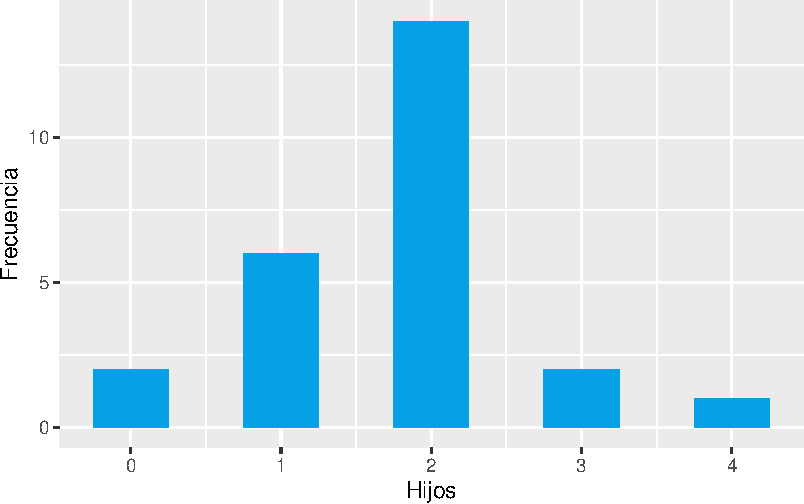
\includegraphics{./estadistica-descriptiva_files/figure-pdf/diagrama-barras-1.pdf}

Y a continuación se muestra el polígono de frecuencias.

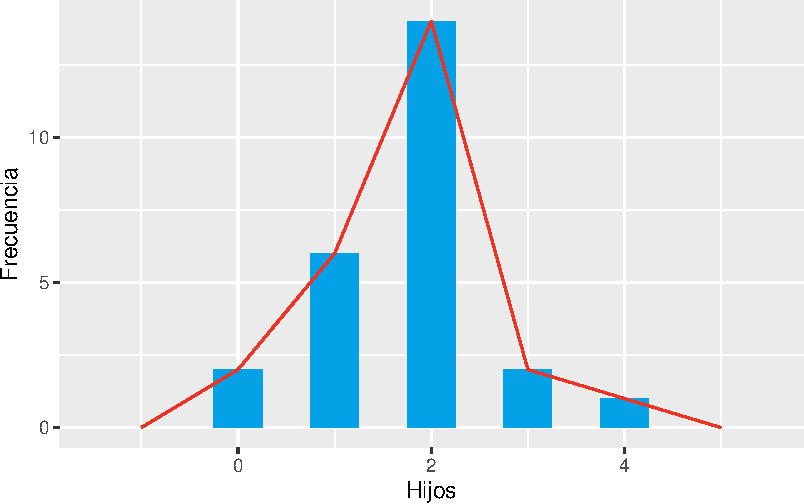
\includegraphics{./estadistica-descriptiva_files/figure-pdf/poligono-frecuencias-absolutas-1.pdf}

El diagrama de barras que aparece a continuación muestra la distribución
de frecuencias relativas del número de hijos en la muestra anterior.

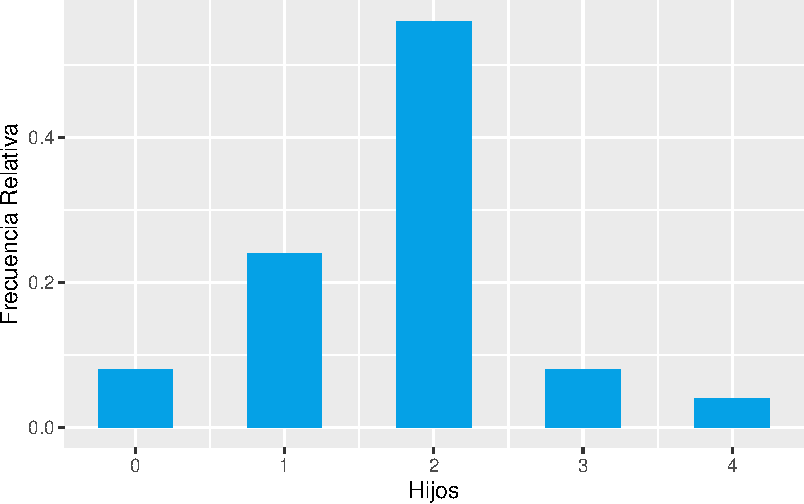
\includegraphics{./estadistica-descriptiva_files/figure-pdf/diagrama-barras-relativas-1.pdf}

El diagrama de barras que aparece a continuación muestra la distribución
de frecuencias absolutas acumuladas del número de hijos en la muestra
anterior.

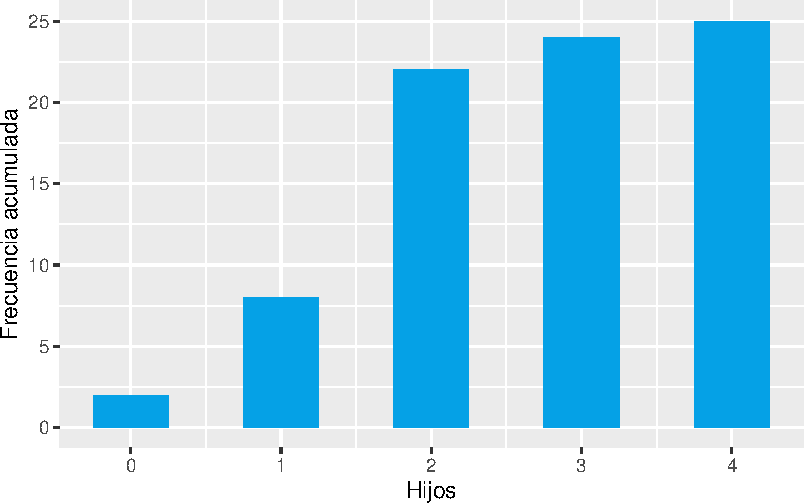
\includegraphics{./estadistica-descriptiva_files/figure-pdf/diagrama-barras-acumuladas-1.pdf}

Y el diagrama de barras que aparece a continuación muestra la
distribución de frecuencias relativas acumuladas del número de hijos en
la muestra anterior.

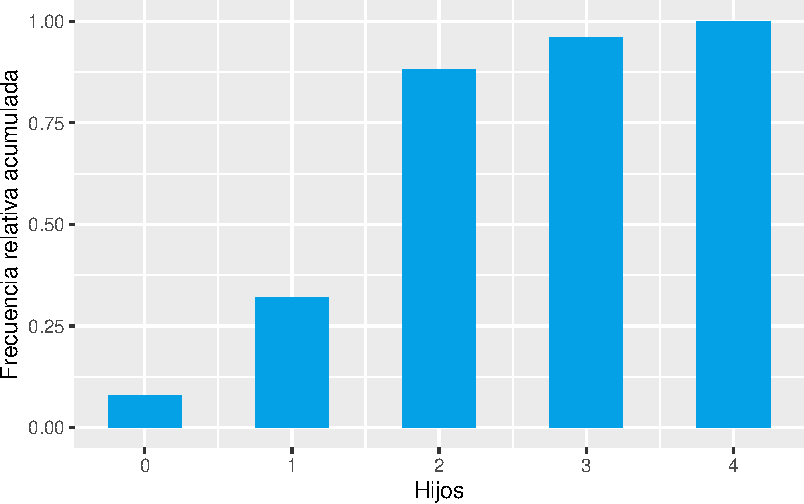
\includegraphics{./estadistica-descriptiva_files/figure-pdf/diagrama-barras-relativas-acumuladas-1.pdf}

Finalmente, el último diagrama muestra el polígono de frecuencias
relativas acumuladas.

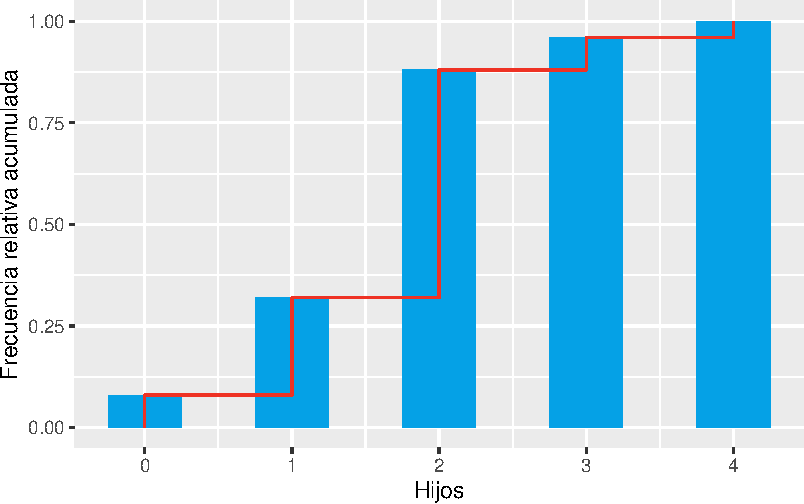
\includegraphics{./estadistica-descriptiva_files/figure-pdf/poligono-relativas-acumuladas-1.pdf}

\end{example}

\hypertarget{histograma}{%
\subsection{Histograma}\label{histograma}}

Un \emph{histograma} es similar a un diagrama de barras pero para datos
agrupados.

Habitualmente las clases o intervalos de agrupación se representan en el
eje \(X\), y las frecuencias en el eje \(Y\). Para cada clase se dibuja
una barra de altura la correspondiente frecuencia. A diferencia del
diagrama de barras, la anchura del la barra coincide con la anchura de
las clases y no hay separación entre dos barras consecutivas.

Dependiendo del tipo de frecuencia representada en el eje \(Y\) existen
distintos tipos de histogramas.

Al igual que con el diagrama de barras, se puede dibujar un
\emph{polígono de frecuencias} uniendo los puntos centrales más altos de
cada barra con segmentos.

\leavevmode\vadjust pre{\hypertarget{exm-histograma}{}}%
\begin{example}[]\label{exm-histograma}

El siguiente histograma muestra la distribución de frecuencias absolutas
de las estaturas.

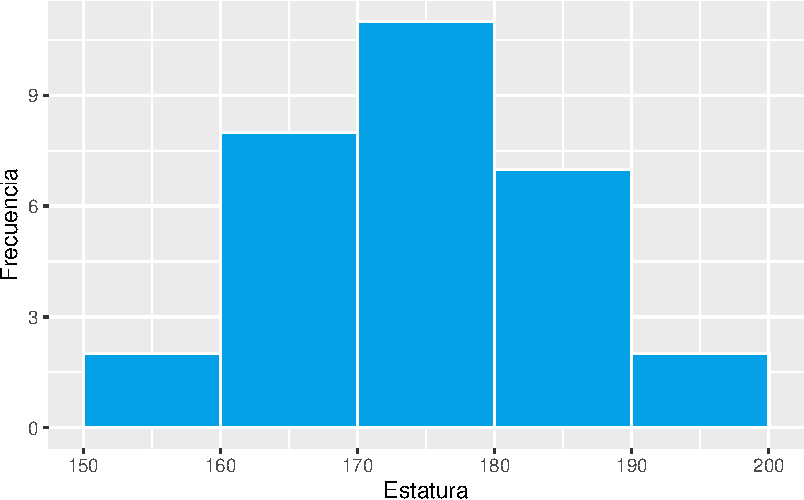
\includegraphics{./estadistica-descriptiva_files/figure-pdf/histograma-1.pdf}

El siguiente histograma muestra la distribución de frecuencias relativas
con el polígono de frecuencias.

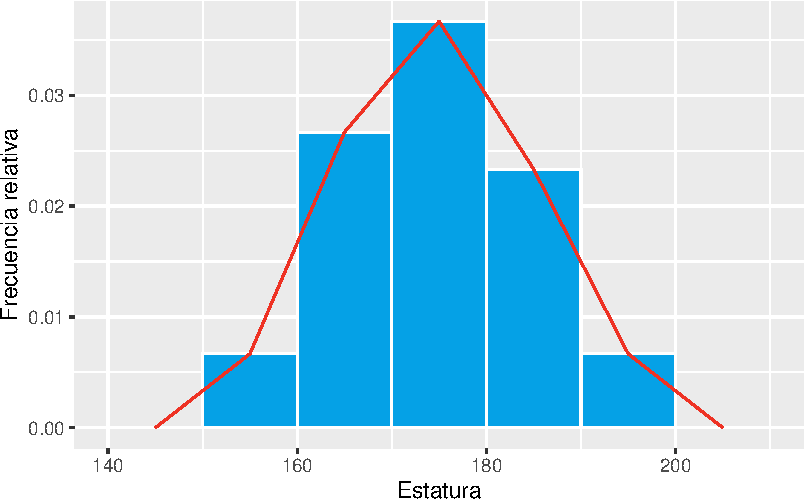
\includegraphics{./estadistica-descriptiva_files/figure-pdf/histograma-frecuencias-relativas-1.pdf}

\end{example}

El polígono de frecuencias acumuladas (absolutas o relativas) se conoce
como \textbf{ojiva}.

\leavevmode\vadjust pre{\hypertarget{exm-ojiva}{}}%
\begin{example}[]\label{exm-ojiva}

El histograma y la ojiva siguientes muestran la distribución de
frecuencias relativas acumuladas de estaturas.

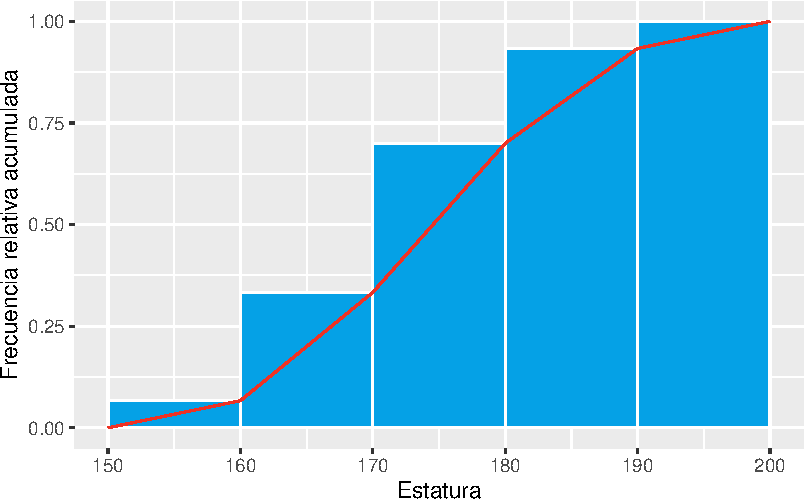
\includegraphics{./estadistica-descriptiva_files/figure-pdf/histograma-frecuencias-relativas-acumuladas-1.pdf}

\end{example}

Obsérvese que en la ojiva se unen los vértices superiores derechos de
cada barra con segmentos, en lugar de los puntos centrales, ya que no se
consigue alcanzar la frecuencia acumulada correspondiente a la clase
hasta que no se alcanza el final del intervalo.

\hypertarget{diagrama-de-sectores}{%
\subsection{Diagrama de sectores}\label{diagrama-de-sectores}}

Un \emph{diagrama de sectores} consiste en un círculo divido en
porciones, uno por cada valor o categoría de la variable. Cada porción
se conoce como \emph{sector} y su ángulo o área es proporcional a la
correspondiente frecuencia del valor o categoría.

Los diagramas de sectores pueden representar frecuencias absolutas o
relativas, pero no pueden representar frecuencias acumuladas, y se
utilizan sobre todo con atributos nominales. Para atributos ordinales o
variables cuantitativas es mejor utilizar diagramas de barras, ya es más
fácil percibir las diferencias en una dimensión (altura de las barras)
que en dos dimensiones (áreas de los sectores).

\leavevmode\vadjust pre{\hypertarget{exm-diagrama-sectores}{}}%
\begin{example}[]\label{exm-diagrama-sectores}

El diagrama de sectores siguiente muestra la distribución de frecuencias
relativas de los grupos sanguíneos.

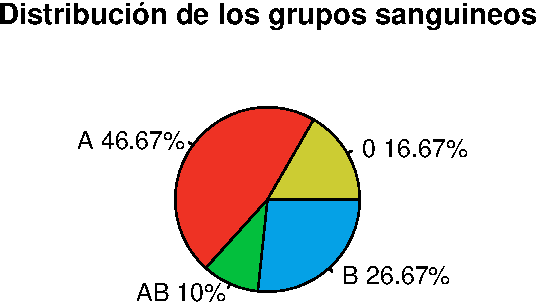
\includegraphics{./estadistica-descriptiva_files/figure-pdf/diagrama-sectores-1.pdf}

\end{example}

\hypertarget{la-distribuciuxf3n-normal}{%
\subsection{La distribución Normal}\label{la-distribuciuxf3n-normal}}

Las distribuciones con diferentes propiedades presentan formas
distintas.

\leavevmode\vadjust pre{\hypertarget{exm-distribucion-ingresos-familiares}{}}%
\begin{example}[Distribución de los ingresos
familiares]\label{exm-distribucion-ingresos-familiares}

~

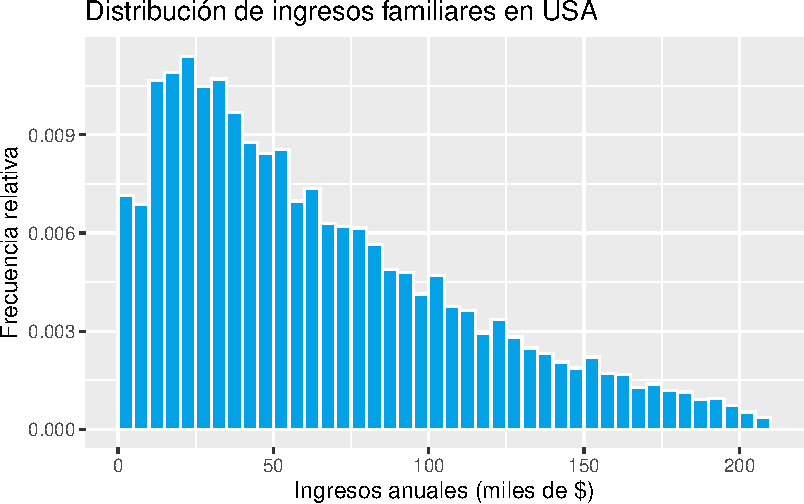
\includegraphics{./estadistica-descriptiva_files/figure-pdf/histograma-ingresos-familiares-1.pdf}

\end{example}

\leavevmode\vadjust pre{\hypertarget{exm-distribucion-edad-fallecimiento}{}}%
\begin{example}[Distribución de la edad de
fallecimiento]\label{exm-distribucion-edad-fallecimiento}

~

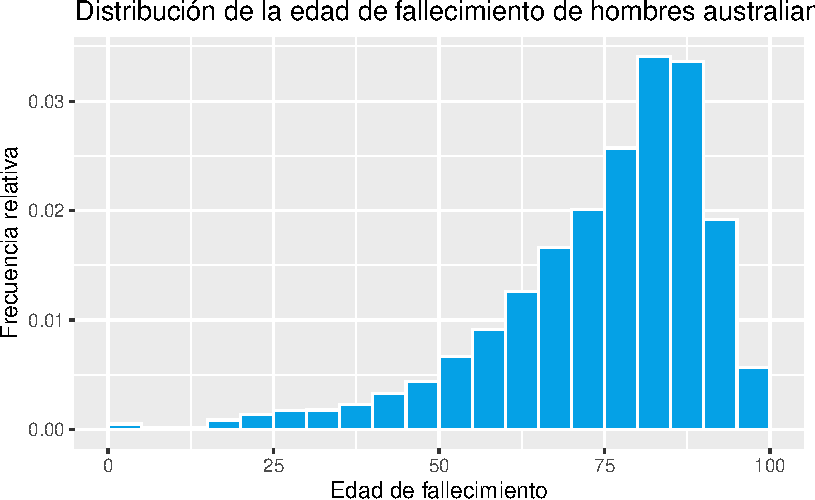
\includegraphics{./estadistica-descriptiva_files/figure-pdf/histograma-edad-fallecimiento-1.pdf}

\end{example}

\leavevmode\vadjust pre{\hypertarget{exm-distribucion-tiempo-espera-metro}{}}%
\begin{example}[Distribución del tiempo de espera del
metro]\label{exm-distribucion-tiempo-espera-metro}

~

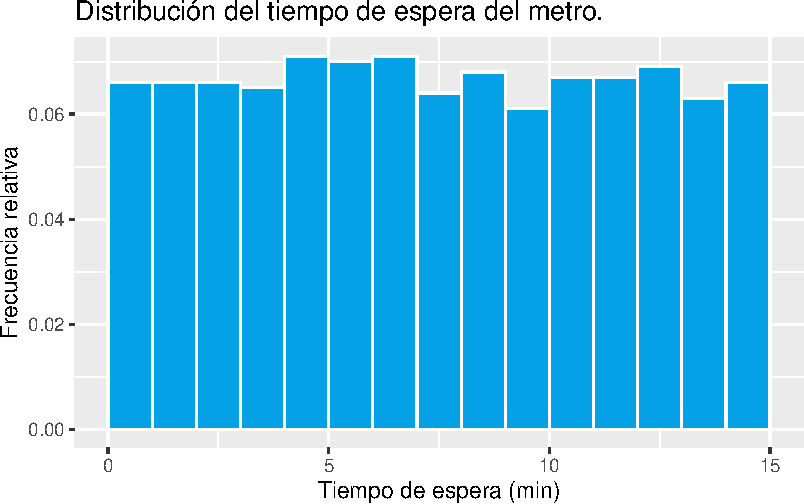
\includegraphics{./estadistica-descriptiva_files/figure-pdf/histograma-tiempo-espera-metro-1.pdf}

\end{example}

\leavevmode\vadjust pre{\hypertarget{exm-distribucion-llegada-clientes-restaurantes}{}}%
\begin{example}[Distribución del tiempo de llegada de clientes a un
restaurante]\label{exm-distribucion-llegada-clientes-restaurantes}

~

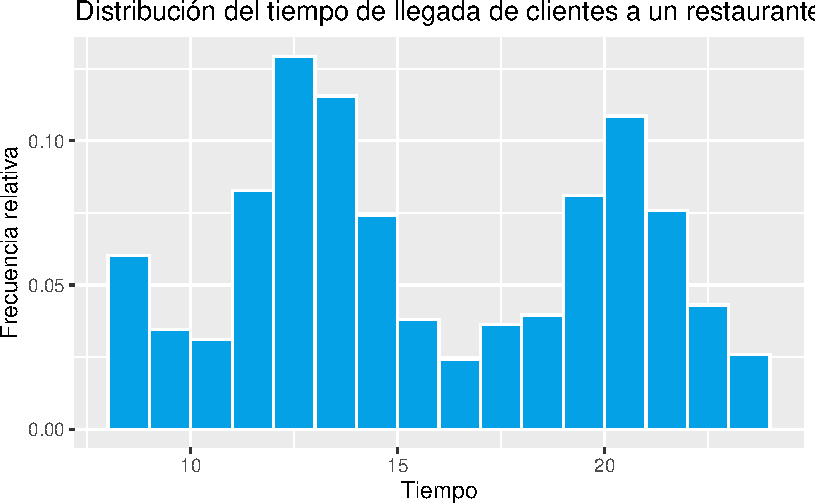
\includegraphics{./estadistica-descriptiva_files/figure-pdf/histograma-tiempo-llegada-restaurante-1.pdf}

\end{example}

Las distribuciones con forma de campana se presentan muy a menudo en las
variables biológicas.

\leavevmode\vadjust pre{\hypertarget{exm-distribucion-peso-hombres}{}}%
\begin{example}[Distribución del peso de los
hombres]\label{exm-distribucion-peso-hombres}

~

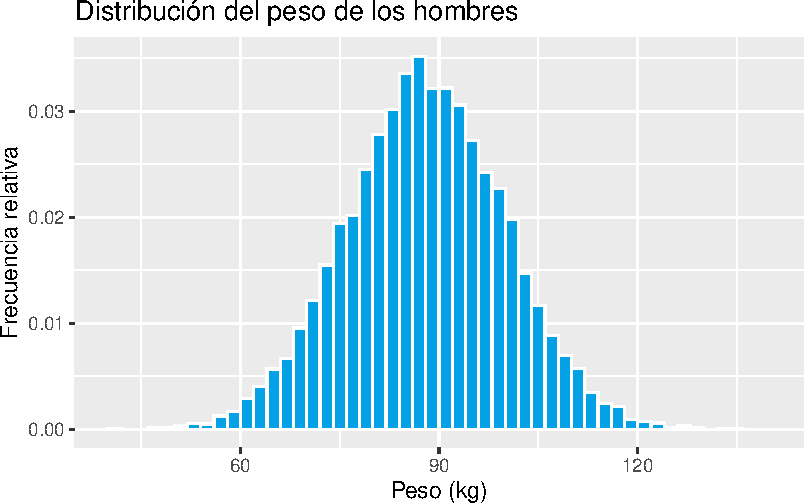
\includegraphics{./estadistica-descriptiva_files/figure-pdf/histograma-peso-hombres-1.pdf}

\end{example}

\leavevmode\vadjust pre{\hypertarget{exm-distribucion-estatura-mujeres}{}}%
\begin{example}[Distribución de la estatura de las
mujeres]\label{exm-distribucion-estatura-mujeres}

~

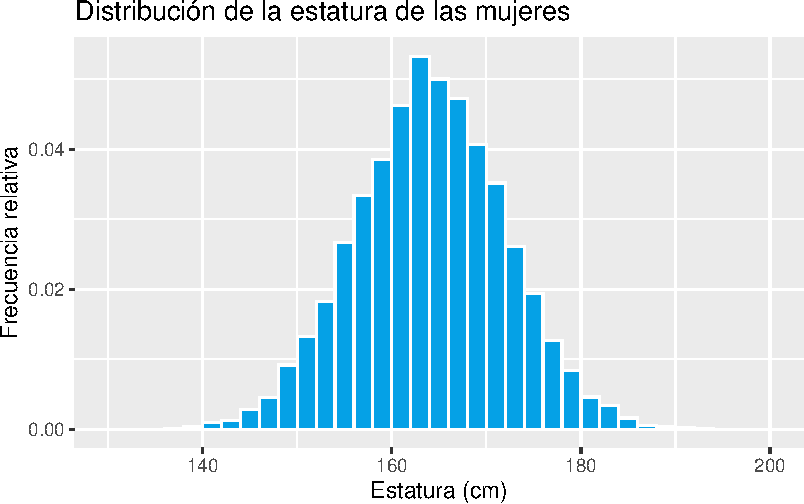
\includegraphics{./estadistica-descriptiva_files/figure-pdf/histograma-estatura-mujeres-1.pdf}

\end{example}

\leavevmode\vadjust pre{\hypertarget{exm-distribucion-estaturas-sexo}{}}%
\begin{example}[Distribución de la estatura según el
sexo]\label{exm-distribucion-estaturas-sexo}

~

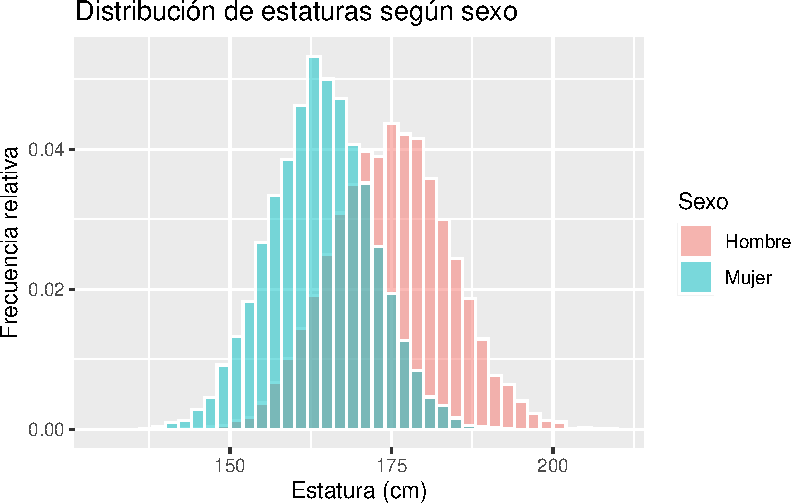
\includegraphics{./estadistica-descriptiva_files/figure-pdf/histograma-estatura-sexo-1.pdf}

\end{example}

\leavevmode\vadjust pre{\hypertarget{exm-distribucion-estaturas-ambos-sexos}{}}%
\begin{example}[Distribución de la estatura de hombres y
mujeres]\label{exm-distribucion-estaturas-ambos-sexos}

~

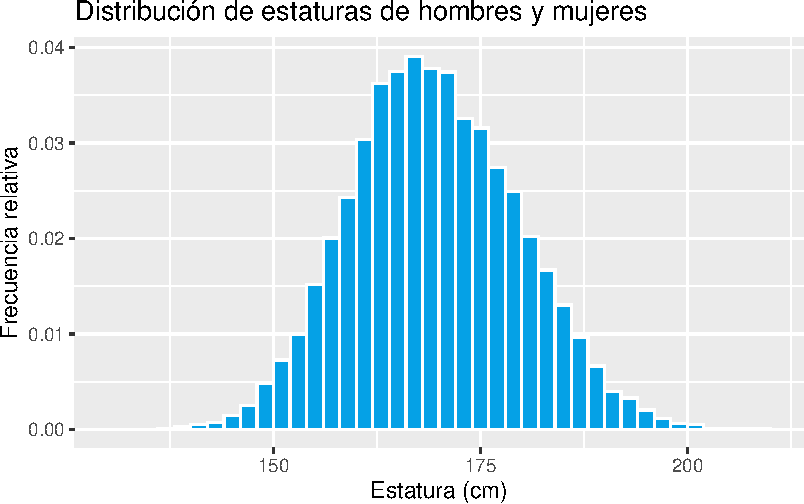
\includegraphics{./estadistica-descriptiva_files/figure-pdf/histograma-estatura-ambos-sexo-1.pdf}

\end{example}

\leavevmode\vadjust pre{\hypertarget{exm-distribucion-colesterol}{}}%
\begin{example}[Distribución del
colesterol]\label{exm-distribucion-colesterol}

~

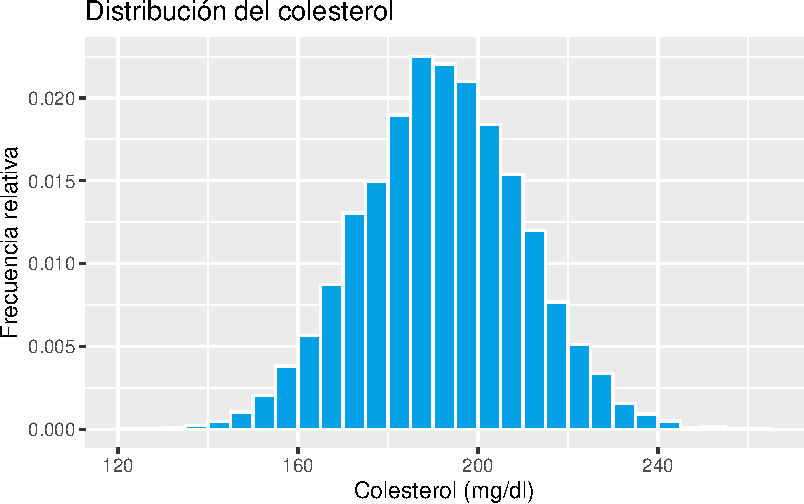
\includegraphics{./estadistica-descriptiva_files/figure-pdf/histograma-colesterol-1.pdf}

\end{example}

\leavevmode\vadjust pre{\hypertarget{exm-distribucion-notas}{}}%
\begin{example}[Distribución de notas]\label{exm-distribucion-notas}

~

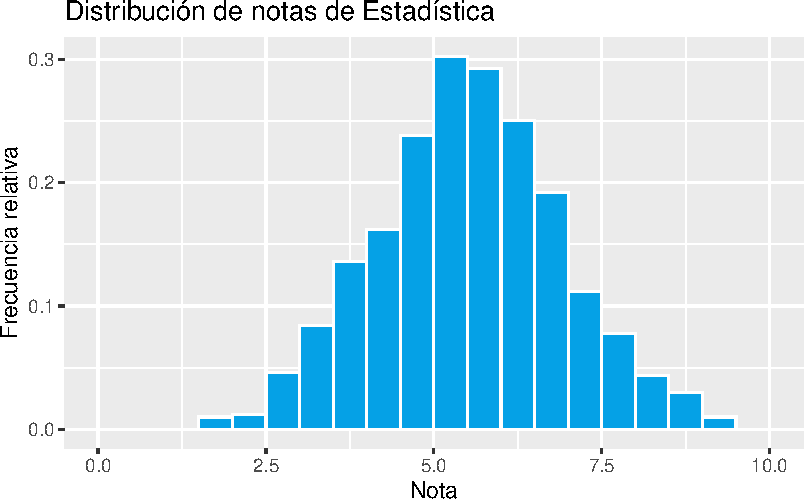
\includegraphics{./estadistica-descriptiva_files/figure-pdf/histograma-notas-1.pdf}

\end{example}

La distribución con forma de campana aparece tan a menudo en la
Naturaleza que se conoce como \emph{distribución normal} o
\emph{distribución gaussiana}.

\begin{figure}

{\centering 

% Created by tikzDevice version 0.12.3 on 2019-09-02 00:52:27
% !TEX encoding = UTF-8 Unicode
\begin{tikzpicture}[x=1pt,y=1pt]
\definecolor{fillColor}{RGB}{255,255,255}
\path[use as bounding box,fill=fillColor,fill opacity=0.00] (0,0) rectangle (505.89,361.35);
\begin{scope}
\path[clip] ( 49.20, 61.20) rectangle (480.69,312.15);
\definecolor{drawColor}{RGB}{238,50,36}

\path[draw=drawColor,line width= 1.2pt,line join=round,line cap=round] ( 65.18, 71.38) --
	( 68.21, 71.54) --
	( 71.23, 71.73) --
	( 74.26, 71.94) --
	( 77.29, 72.18) --
	( 80.31, 72.46) --
	( 83.34, 72.78) --
	( 86.37, 73.15) --
	( 89.39, 73.57) --
	( 92.42, 74.04) --
	( 95.45, 74.58) --
	( 98.48, 75.19) --
	(101.50, 75.88) --
	(104.53, 76.65) --
	(107.56, 77.51) --
	(110.58, 78.47) --
	(113.61, 79.55) --
	(116.64, 80.74) --
	(119.66, 82.06) --
	(122.69, 83.52) --
	(125.72, 85.12) --
	(128.74, 86.88) --
	(131.77, 88.81) --
	(134.80, 90.92) --
	(137.82, 93.21) --
	(140.85, 95.69) --
	(143.88, 98.37) --
	(146.90,101.27) --
	(149.93,104.38) --
	(152.96,107.71) --
	(155.98,111.26) --
	(159.01,115.04) --
	(162.04,119.06) --
	(165.06,123.30) --
	(168.09,127.77) --
	(171.12,132.46) --
	(174.14,137.37) --
	(177.17,142.49) --
	(180.20,147.81) --
	(183.22,153.31) --
	(186.25,158.98) --
	(189.28,164.81) --
	(192.30,170.76) --
	(195.33,176.83) --
	(198.36,182.98) --
	(201.38,189.20) --
	(204.41,195.44) --
	(207.44,201.68) --
	(210.46,207.89) --
	(213.49,214.03) --
	(216.52,220.08) --
	(219.54,225.99) --
	(222.57,231.73) --
	(225.60,237.26) --
	(228.62,242.56) --
	(231.65,247.58) --
	(234.68,252.29) --
	(237.70,256.66) --
	(240.73,260.65) --
	(243.76,264.25) --
	(246.78,267.43) --
	(249.81,270.15) --
	(252.84,272.41) --
	(255.86,274.19) --
	(258.89,275.46) --
	(261.92,276.23) --
	(264.94,276.49) --
	(267.97,276.23) --
	(271.00,275.46) --
	(274.03,274.19) --
	(277.05,272.41) --
	(280.08,270.15) --
	(283.11,267.43) --
	(286.13,264.25) --
	(289.16,260.65) --
	(292.19,256.66) --
	(295.21,252.29) --
	(298.24,247.58) --
	(301.27,242.56) --
	(304.29,237.26) --
	(307.32,231.73) --
	(310.35,225.99) --
	(313.37,220.08) --
	(316.40,214.03) --
	(319.43,207.89) --
	(322.45,201.68) --
	(325.48,195.44) --
	(328.51,189.20) --
	(331.53,182.98) --
	(334.56,176.83) --
	(337.59,170.76) --
	(340.61,164.81) --
	(343.64,158.98) --
	(346.67,153.31) --
	(349.69,147.81) --
	(352.72,142.49) --
	(355.75,137.37) --
	(358.77,132.46) --
	(361.80,127.77) --
	(364.83,123.30) --
	(367.85,119.06) --
	(370.88,115.04) --
	(373.91,111.26) --
	(376.93,107.71) --
	(379.96,104.38) --
	(382.99,101.27) --
	(386.01, 98.37) --
	(389.04, 95.69) --
	(392.07, 93.21) --
	(395.09, 90.92) --
	(398.12, 88.81) --
	(401.15, 86.88) --
	(404.17, 85.12) --
	(407.20, 83.52) --
	(410.23, 82.06) --
	(413.25, 80.74) --
	(416.28, 79.55) --
	(419.31, 78.47) --
	(422.33, 77.51) --
	(425.36, 76.65) --
	(428.39, 75.88) --
	(431.41, 75.19) --
	(434.44, 74.58) --
	(437.47, 74.04) --
	(440.50, 73.57) --
	(443.52, 73.15) --
	(446.55, 72.78) --
	(449.58, 72.46) --
	(452.60, 72.18) --
	(455.63, 71.94) --
	(458.66, 71.73) --
	(461.68, 71.54) --
	(464.71, 71.38);
\end{scope}
\begin{scope}
\path[clip] (  0.00,  0.00) rectangle (505.89,361.35);
\definecolor{drawColor}{RGB}{0,0,0}

\node[text=drawColor,anchor=base,inner sep=0pt, outer sep=0pt, scale=  1.20] at (264.94,332.61) {\bfseries Gauss bell};
\end{scope}
\end{tikzpicture}


}

\caption{Campana de Gauss.}

\end{figure}

\hypertarget{datos-atuxedpicos}{%
\section{Datos atípicos}\label{datos-atuxedpicos}}

Uno de los principales problemas de las muestras son los \textbf{datos
atípicos}, que son valores de la variable que se diferencian mucho del
resto de los valores en la muestra.

\begin{figure}

{\centering 
\includegraphics{./img/descriptiva/dato_atipico.png}

}

\caption{Dato atípico.}

\end{figure}

Es muy importante detectar los datos atípicos antes de realizar
cualquier análisis de los datos, pues suelen distorsionar los
resultados.

Aparecen siempre en los extremos de la distribución, y pueden detectarse
con un diagrama de caja y bigotes (tal y como veremos más adelante).

\hypertarget{tratamiento-de-los-datos-atuxedpicos}{%
\subsection{Tratamiento de los datos
atípicos}\label{tratamiento-de-los-datos-atuxedpicos}}

Cuando trabajemos con muestras grandes, los datos atípicos tienen menor
influencia y pueden dejarse en la muestra.

Cuando trabajemos con muestras pequeñas tenemos varias opciones:

\begin{itemize}
\tightlist
\item
  Eliminar el dato atípico si se trata de un error.
\item
  Sustituir el dato atípico por el menor o el mayor valor de la
  distribución que no es atípico si no se trata de un error y el dato
  atípico no concuerda con la distribución teórica.
\item
  Dejar el dato atípico si no es un error, y cambiar el modelo de
  distribución teórico para adecuarlo a los datos atípicos.
\end{itemize}

\hypertarget{estaduxedsticos-muestrales}{%
\section{Estadísticos muestrales}\label{estaduxedsticos-muestrales}}

La tabla de frecuencias sintetiza la información de la distribución de
valores de la variable estudiada en la muestra, pero en muchas ocasiones
es insuficiente para describir determinados aspectos de la distribución,
como por ejemplo, cuáles son los valores más representativos de la
muestra, cómo es la variabilidad de los datos, qué datos pueden
considerarse atípicos, o cómo es la simetría de la distribución.

Para describir esos aspectos de la distribución muestral se utilizan
unas medidas resumen llamadas \textbf{estadísticos muestrales}.

De acuerdo al aspecto de las distribución que miden, existen diferentes
tipos de estadísticos:

\textbf{Estadísticos de Posición}: Miden los valores en torno a los que
se agrupan los datos o que dividen la distribución en partes iguales.

\textbf{Estadísticos de Dispersión}: Miden la heterogeneidad de los
datos.

\textbf{Estadísticos de Forma}: Miden aspectos de la forma que tiene la
distribución de los datos, como la simetría o el apuntamiento.

\hypertarget{estaduxedsticos-de-posiciuxf3n}{%
\section{Estadísticos de
posición}\label{estaduxedsticos-de-posiciuxf3n}}

Pueden ser de dos tipos:

\textbf{Estadísticos de Tendencia Central}: Determinan valores alrededor
de los cuales se concentran los datos, habitualmente en el centro de la
distribución. Estas medidas suelen utilizarse como valores
representativos de la muestra. Las más importantes son:

\begin{itemize}
\tightlist
\item
  Media aritmética
\item
  Mediana
\item
  Moda
\end{itemize}

\textbf{Estadísticos de Posición no centrales}: Dividen la distribución
en partes con el mismo número de datos. Las más importantes son:

\begin{itemize}
\tightlist
\item
  Cuartiles.
\item
  Deciles.
\item
  Percentiles.
\end{itemize}

\hypertarget{media-aritmuxe9tica}{%
\subsection{Media aritmética}\label{media-aritmuxe9tica}}

\leavevmode\vadjust pre{\hypertarget{def-media-aritmetica}{}}%
\begin{definition}[Media aritmética muestral
\(\bar{x}\)]\label{def-media-aritmetica}

La \emph{media aritmética muestral} de una variable \(X\) es la suma de
los valores observados en la muestra dividida por el tamaño muestral

\[\bar{x} = \frac{\sum x_i}{n}\]

\end{definition}

A partir de la tabla de frecuencias puede calcularse con la fórmula

\[\bar{x} = \frac{\sum x_in_i}{n} = \sum x_i f_i\]

En la mayoría de los casos, la media aritmética es la medida que mejor
representa a la muestra.

\begin{tcolorbox}[enhanced jigsaw, coltitle=black, breakable, bottomrule=.15mm, colback=white, bottomtitle=1mm, toprule=.15mm, opacitybacktitle=0.6, titlerule=0mm, toptitle=1mm, title=\textcolor{quarto-callout-warning-color}{\faExclamationTriangle}\hspace{0.5em}{Advertencia}, colframe=quarto-callout-warning-color-frame, opacityback=0, arc=.35mm, left=2mm, rightrule=.15mm, leftrule=.75mm, colbacktitle=quarto-callout-warning-color!10!white]

No puede calcularse para variables cualitativas.

\end{tcolorbox}

\leavevmode\vadjust pre{\hypertarget{exm-media-datos-no-agrupados}{}}%
\begin{example}[Datos no agrupados]\label{exm-media-datos-no-agrupados}

Utilizando los datos de la muestra del número de hijos en las familias,
la media aritmética es

\[
\begin{aligned}
\bar{x} &= \frac{1+2+4+2+2+2+3+2+1+1+0+2+2}{25}+\\
 &+\frac{0+2+2+1+2+2+3+1+2+2+1+2}{25} = \frac{44}{25} = 1.76 \mbox{ hijos}.
\end{aligned}
\]

o bien, desde la tabla de frecuencias

\[
\begin{array}{rrrrr}
\hline
x_i & n_i & f_i & x_in_i & x_if_i\\
\hline
0 & 2 & 0.08 & 0 & 0\\
1 & 6 & 0.24 & 6 & 0.24\\
2 & 14 & 0.56 & 28 & 1.12\\
3 & 2  & 0.08 & 6 & 0.24\\
4 & 1 & 0.04 & 4 & 0.16 \\
\hline
\sum & 25 & 1 & 44 & 1.76 \\
\hline
\end{array}
\]

\[
\bar{x} = \frac{\sum x_in_i}{n} = \frac{44}{25}= 1.76 \mbox{ hijos}\qquad \bar{x}=\sum{x_if_i} = 1.76 \mbox{ hijos}.
\]

Esto significa que el valor que mejor representa el número de hijos en
las familias de la muestra es 1.76 hijos.

\end{example}

\leavevmode\vadjust pre{\hypertarget{exm-media-datos-agrupados}{}}%
\begin{example}[Datos agrupados]\label{exm-media-datos-agrupados}

Utilizando los datos de la muestra de estaturas, la media es

\[
\bar{x} = \frac{179+173+\cdots+187}{30} = 175.07 \mbox{ cm}.
\]

o bien, desde la tabla de frecuencias utilizando las marcas de clase
\(x_i\):

\[
\begin{array}{crrrrr}
\hline
X & x_i & n_i & f_i & x_in_i & x_if_i\\
\hline
(150,160] & 155 & 2 & 0.07 & 310 & 10.33\\
(160,170] & 165 & 8 & 0.27 & 1320 & 44.00\\
(170,180] & 175 & 11 & 0.36 & 1925 & 64.17\\
(180,190] & 185 & 7 & 0.23 & 1295 & 43.17\\
(190,200] & 195 & 2 & 0.07 & 390 & 13 \\
\hline
\sum &  & 30 & 1 & 5240 & 174.67 \\
\hline
\end{array}
\]

\[
\bar{x} = \frac{\sum x_in_i}{n} = \frac{5240}{30}= 174.67 \mbox{ cm} \qquad \bar{x}=\sum{x_if_i} = 174.67 \mbox{ cm}.
\]

Obsérvese que al calcular la media desde la tabla de frecuencias el
resultado difiere ligeramente del valor real obtenido directamente desde
la muestra, ya que los valores usados en los cálculos no son los datos
reales sino las marcas de clase.

\end{example}

\hypertarget{media-ponderada}{%
\subsubsection{Media ponderada}\label{media-ponderada}}

En algunos casos, los valores de la muestra no tienen la misma
importancia. En este caso la importancia o \emph{peso} de cada valor de
la muestra debe tenerse en cuenta al calcular la media.

\leavevmode\vadjust pre{\hypertarget{def-media-ponderada}{}}%
\begin{definition}[Media ponderada muestral
\(\bar x_p\)]\label{def-media-ponderada}

Dada una muestra de valores \(x_1,\ldots, x_n\) donde cada valor \(x_i\)
tiene asociado un peso \(p_i\), la \emph{media ponderada muestral} de la
variable \(X\) es la suma de los productos de cada valor observado en la
muestra por su peso, dividida por la suma de todos los pesos

\[\bar{x}_p = \frac{\sum x_ip_i}{\sum p_i}\]

\end{definition}

A partir de la tabla de frecuencias puede calcularse con la fórmula

\[\bar{x}_p = \frac{\sum x_ip_in_i}{\sum p_i}\]

\leavevmode\vadjust pre{\hypertarget{exm-media-ponderada}{}}%
\begin{example}[]\label{exm-media-ponderada}

Supóngase que un estudiante quiere calcular una medida que represente su
rendimiento en el curso. La nota obtenida en cada asignatura y sus
créditos son

\begin{longtable}[]{@{}ccl@{}}
\toprule()
Asignatura & Créditos & Nota \\
\midrule()
\endhead
Matemáticas & 6 & 5 \\
Economía & 4 & 3 \\
Química & 8 & 6 \\
\bottomrule()
\end{longtable}

La media aritmética vale

\[\bar{x} = \frac{\sum x_i}{n} = \frac{5+3+6}{3}= 4.67 \text{ puntos}.\]

Sin embargo, esta nota no representa bien el rendimiento académico del
alumno ya que no todas las asignaturas tienen la misma importancia ni
requieren el mismo esfuerzo para aprobar. Las asignaturas con más
créditos requieren más trabajo y deben tener más peso en el cálculo de
la media.

Es más lógico usar la media ponderada como medida del rendimiento del
estudiante, tomando como pesos los créditos de cada asignatura

\[
\bar{x}_p = \frac{\sum x_ip_i}{\sum p_i} = \frac{5\cdot 6+3\cdot 4+6\cdot 8}{6+4+8}= \frac{90}{18} = 5 \text{ puntos}.
\]

\end{example}

\hypertarget{mediana}{%
\subsection{Mediana}\label{mediana}}

\leavevmode\vadjust pre{\hypertarget{def-mediana}{}}%
\begin{definition}[Mediana muestral \(Me\)]\label{def-mediana}

La \emph{mediana muestral} de una variable \(X\) es el valor de la
variable que está en el medio de la muestra ordenada.

\end{definition}

La mediana divide la distribución de la muestra en dos partes iguales,
es decir, hay el mismo número de valores por debajo y por encima de la
mediana. Por tanto, tiene frecuencias acumuladas \(N_{Me}= n/2\) y
\(F_{Me}= 0.5\).

\begin{tcolorbox}[enhanced jigsaw, coltitle=black, breakable, bottomrule=.15mm, colback=white, bottomtitle=1mm, toprule=.15mm, opacitybacktitle=0.6, titlerule=0mm, toptitle=1mm, title=\textcolor{quarto-callout-warning-color}{\faExclamationTriangle}\hspace{0.5em}{Advertencia}, colframe=quarto-callout-warning-color-frame, opacityback=0, arc=.35mm, left=2mm, rightrule=.15mm, leftrule=.75mm, colbacktitle=quarto-callout-warning-color!10!white]

No puede calcularse para variables nominales.

\end{tcolorbox}

Con datos no agrupados pueden darse varios casos:

\begin{itemize}
\tightlist
\item
  Tamaño muestral impar: La mediana es el valor que ocupa la posición
  \(\frac{n+1}{2}\).
\item
  Tamaño muestral par: La mediana es la media de los valores que ocupan
  las posiciones \(\frac{n}{2}\) y \(\frac{n}{2}+1\).
\end{itemize}

\begin{figure}

{\centering 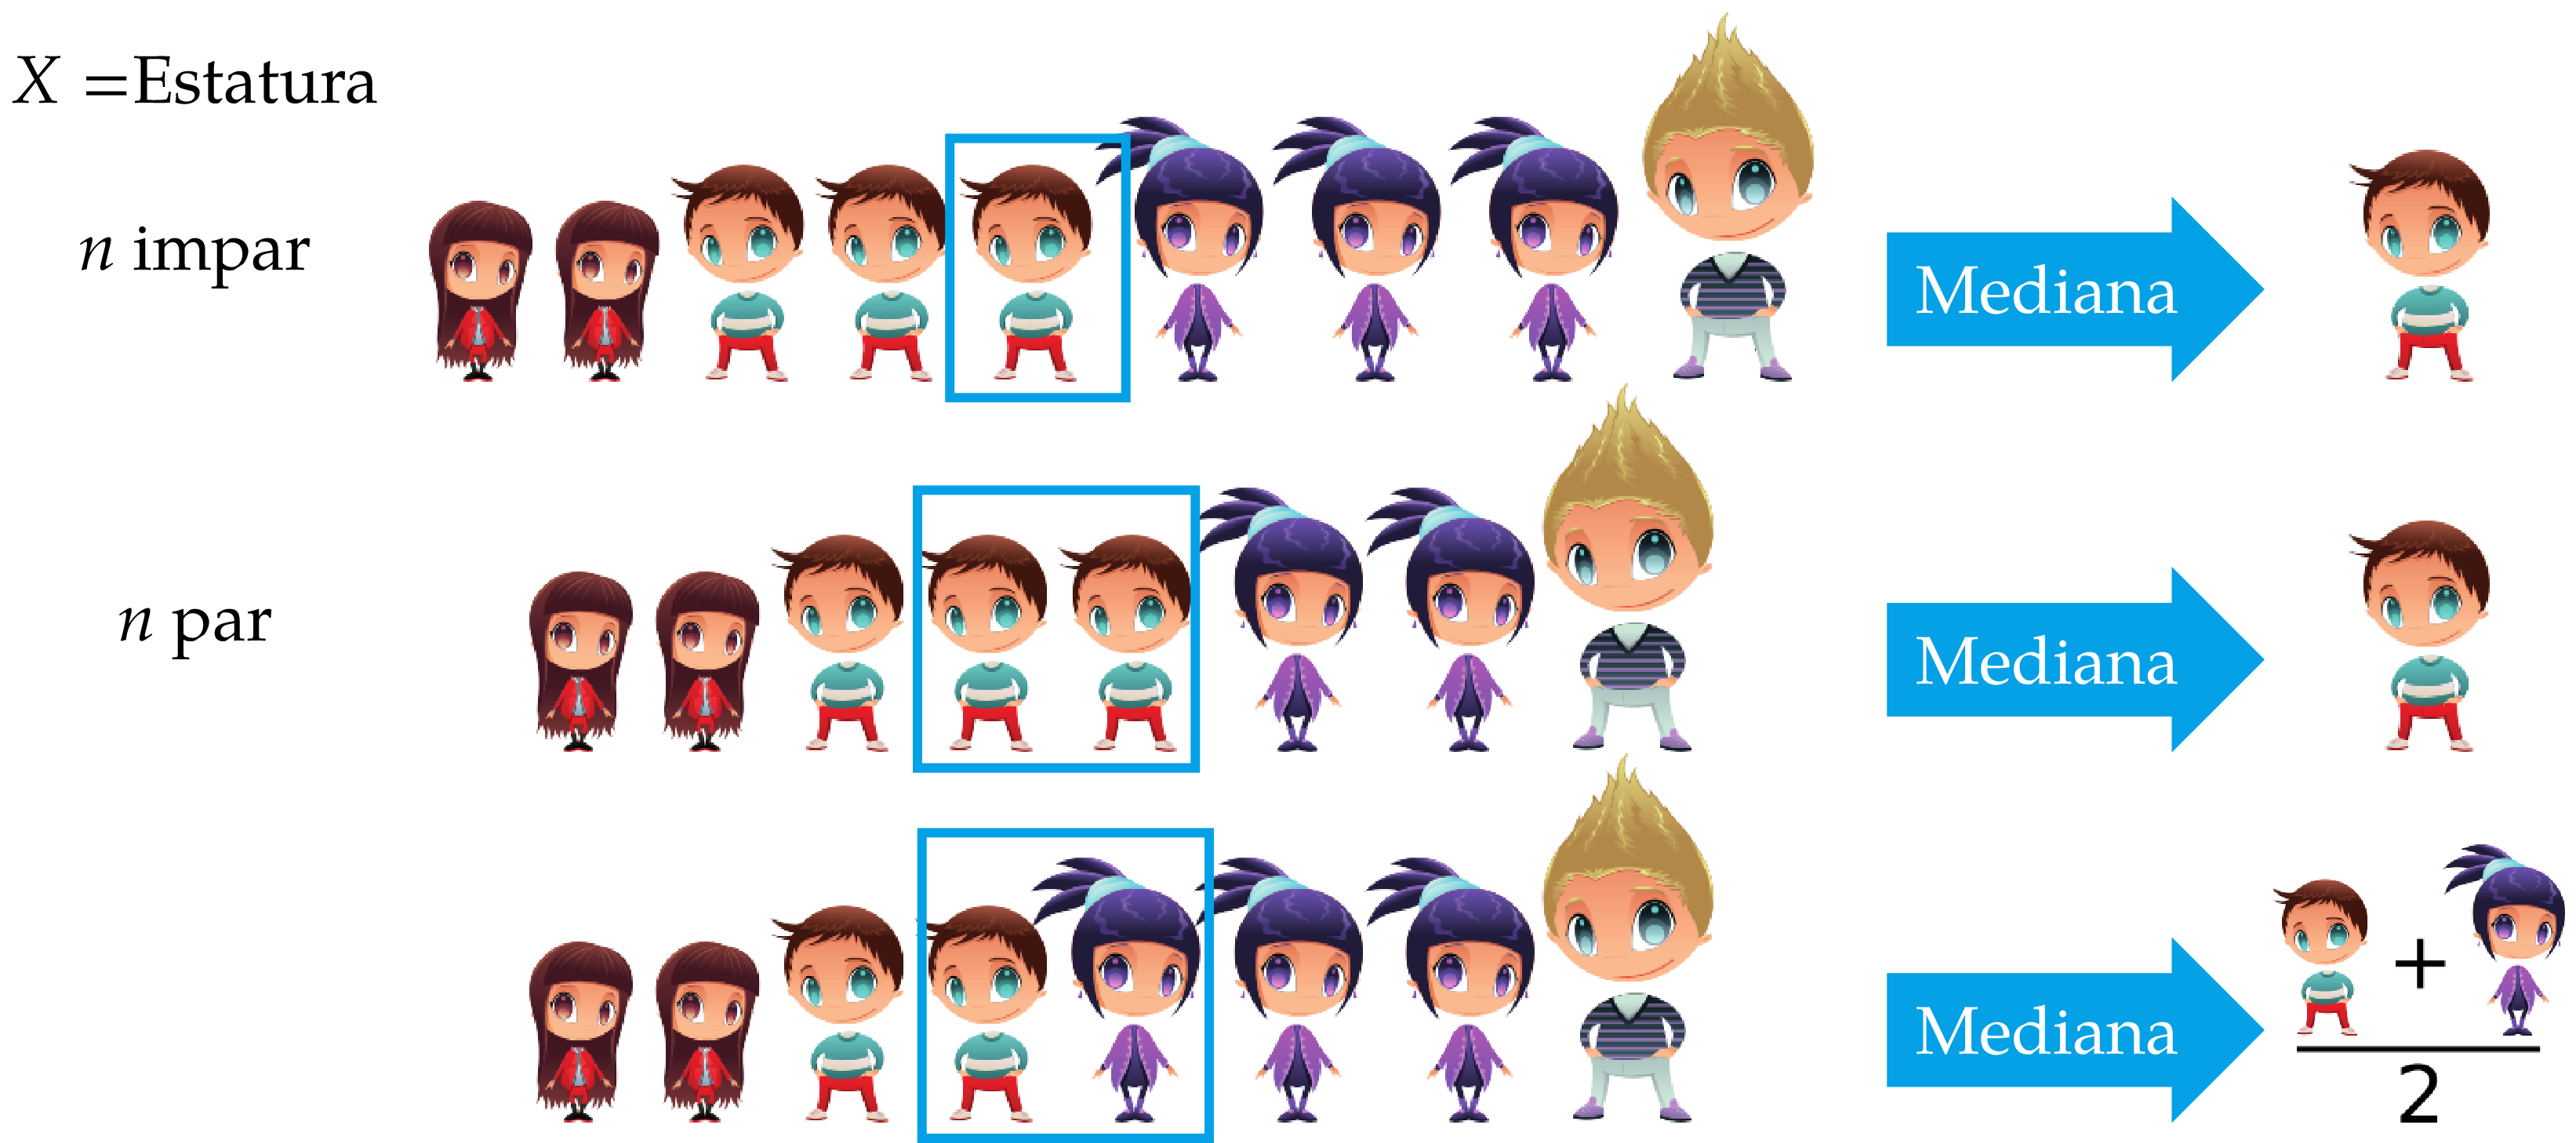
\includegraphics{./img/descriptiva/mediana.png}

}

\caption{Cálculo de la mediana con datos no agrupados.}

\end{figure}

:::\{\#exm-mediana-datos-no-agrupados\} Utilizando los datos del número
de hijos de las familias, el tamaño muestral es 25, que es impar, y la
mediana es el valor que ocupa la posición \(\frac{25+1}{2} = 13\) de la
muestra ordenada.

\[
0,0,1,1,1,1,1,1,2,2,2,2,\fbox{2},2,2,2,2,2,2,2,2,2,3,3,4
\]

y la mediana es 2 hijos.

Si se trabaja con la tabla de frecuencias, la mediana es el valor más
pequeño con una frecuencia acumulada mayor o igual a \(13\), o con una
frecuencia relativa acumulada mayor o igual que \(0.5\).

\[
\begin{array}{rrrrr}
\hline
x_i & n_i & f_i & N_i & F_i\\
\hline
0 & 2 & 0.08 & 2 & 0.08\\
1 & 6 & 0.24 & 8 & 0.32\\
\color{red}2 & 14 & 0.56 & 22 & 0.88\\
3 & 2  & 0.08 & 24 & 0.96\\
4 & 1 & 0.04 & 25 & 1 \\
\hline
\sum & 25 & 1 \\
\hline
\end{array}
\]

\hypertarget{cuxe1lculo-de-la-mediana-con-datos-agrupados}{%
\subsubsection{Cálculo de la mediana con datos
agrupados}\label{cuxe1lculo-de-la-mediana-con-datos-agrupados}}

Con datos agrupados la mediana se calcula interpolando en el polígono de
frecuencias relativas acumuladas para el valor 0.5.

\begin{figure}

{\centering 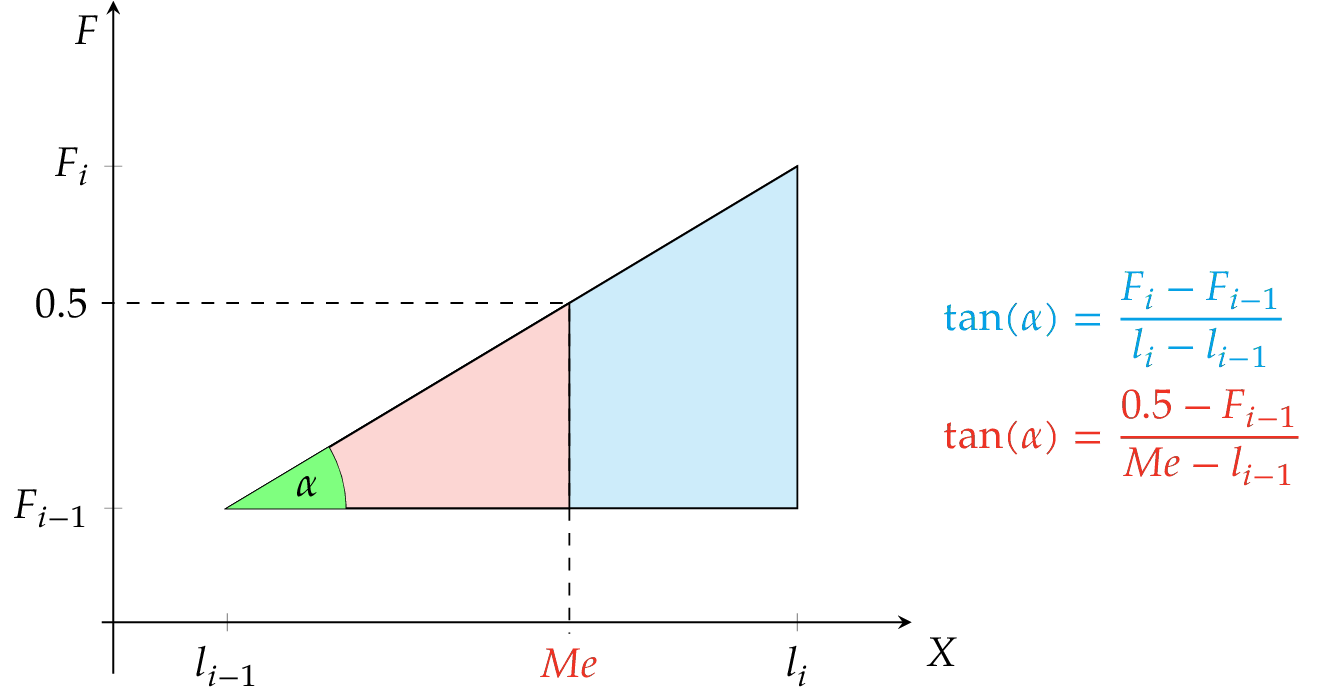
\includegraphics{./img/descriptiva/interpolacion.png}

}

\caption{Cálculo de la mediana con datos agrupados.}

\end{figure}

Ambas expresiones son iguales ya que el ángulo \(\alpha\) es el mismo, y
resolviendo la ecuación se tiene la siguiente fórmula para calcular la
mediana

\[
Me=l_i+\frac{0.5-F_{i-1}}{F_i-F_{i-1}}(l_i-l_{i-1})=l_i+\frac{0.5-F_{i-1}}{f_i}a_i
\]

\leavevmode\vadjust pre{\hypertarget{exm-mediana-datos-agrupados}{}}%
\begin{example}[Datos agrupados]\label{exm-mediana-datos-agrupados}

Utilizando los datos de la muestra de las estaturas de estudiantes, la
mediana cae en la clase (170,180{]}.

\begin{figure}

{\centering 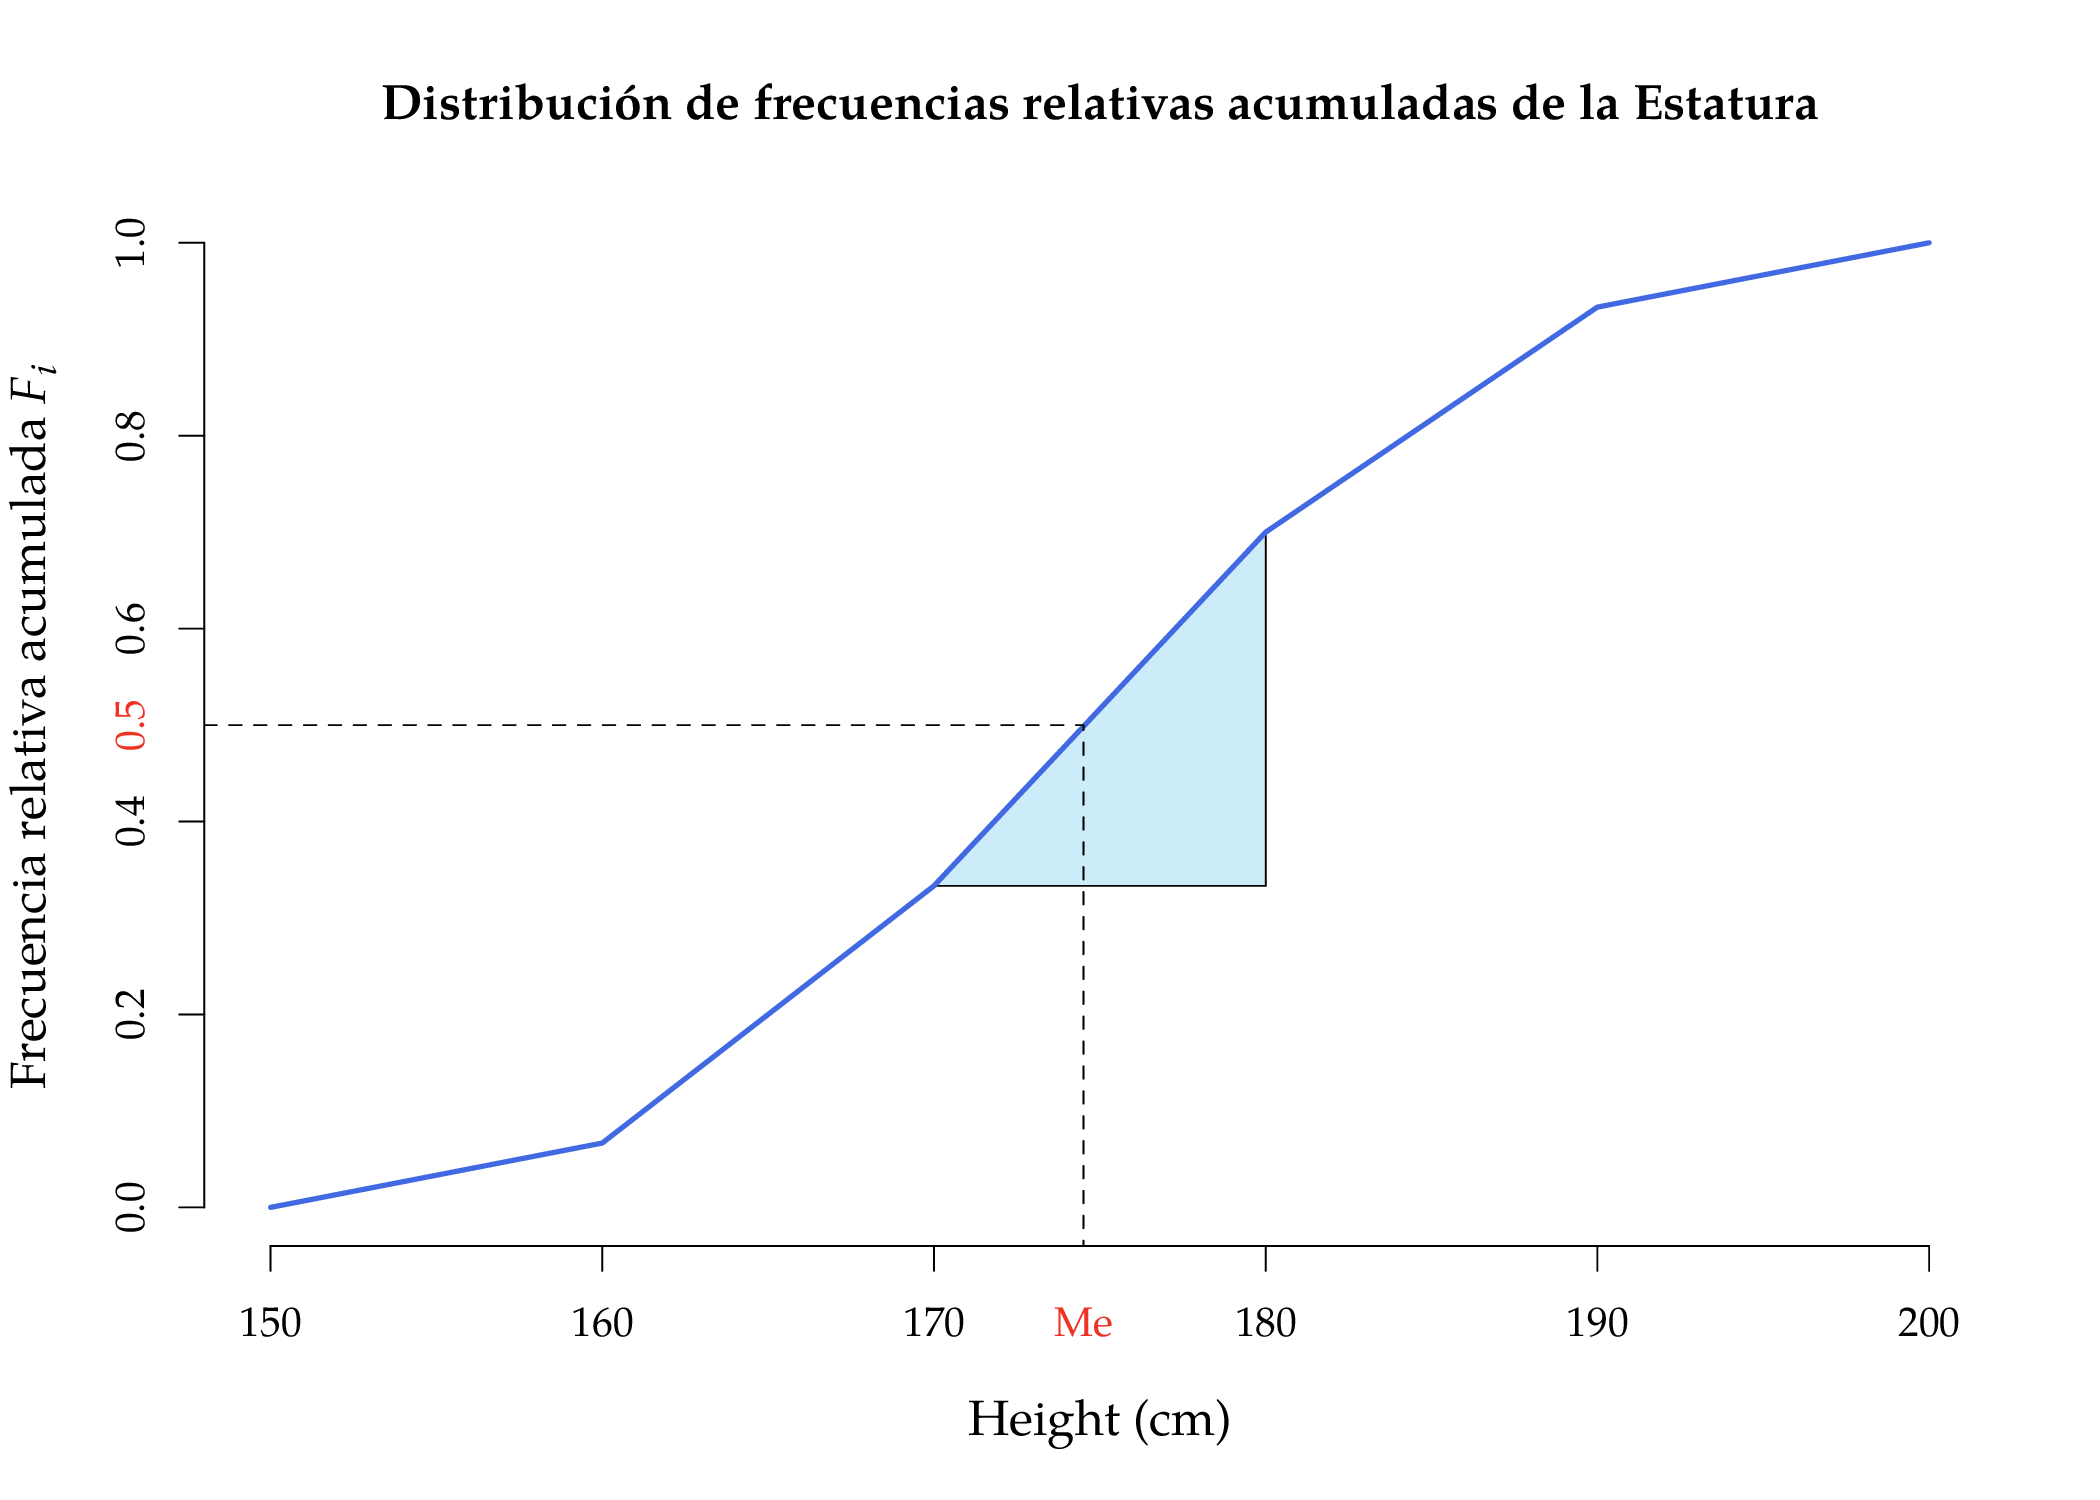
\includegraphics{./img/descriptiva/interpolacion_ejemplo_1.png}

}

\caption{Ejemplo de cálculo de la mediana con datos agrupados.}

\end{figure}

Interpolando en el intervalo (170,180{]} se tiene

\begin{figure}

{\centering 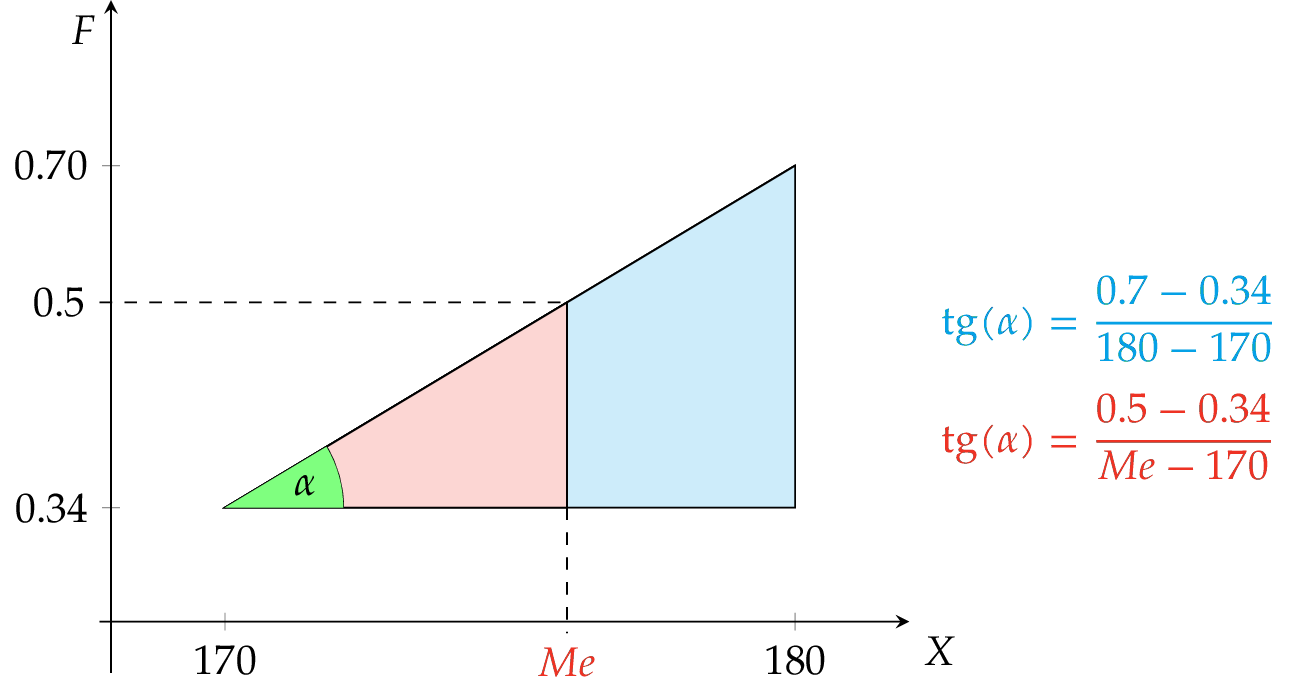
\includegraphics{./img/descriptiva/interpolacion_ejemplo_2.png}

}

\caption{Ejemplo de cálculo de la mediana con datos agrupados.}

\end{figure}

Igualando ambas expresiones y resolviendo la ecuación se obtiene

\[
Me= 170+\frac{0.5-0.34}{0.7-0.34}(180-170)=170+\frac{0.16}{0.36}10=174.54 \mbox{ cm}.
\]

Esto significa que la mitad de los estudiantes tienen estaturas menores
o iguales que 174.54 cm y la otra mitad mayores o iguales.

\end{example}

\hypertarget{moda}{%
\subsection{Moda}\label{moda}}

\leavevmode\vadjust pre{\hypertarget{def-moda}{}}%
\begin{definition}[Moda muestral \(Mo\)]\label{def-moda}

La \emph{moda muestral} de una variable \(X\) es el valor de la variable
más frecuente en la muestra.

\end{definition}

Con datos agrupados la \emph{clase modal} es la clase con mayor
frecuencia en la muestra.

Puede calcularse para todos los tipos de variables (cuantitativas y
cualitativas).

Las distribuciones pueden tener más de una moda.

\begin{figure}

{\centering 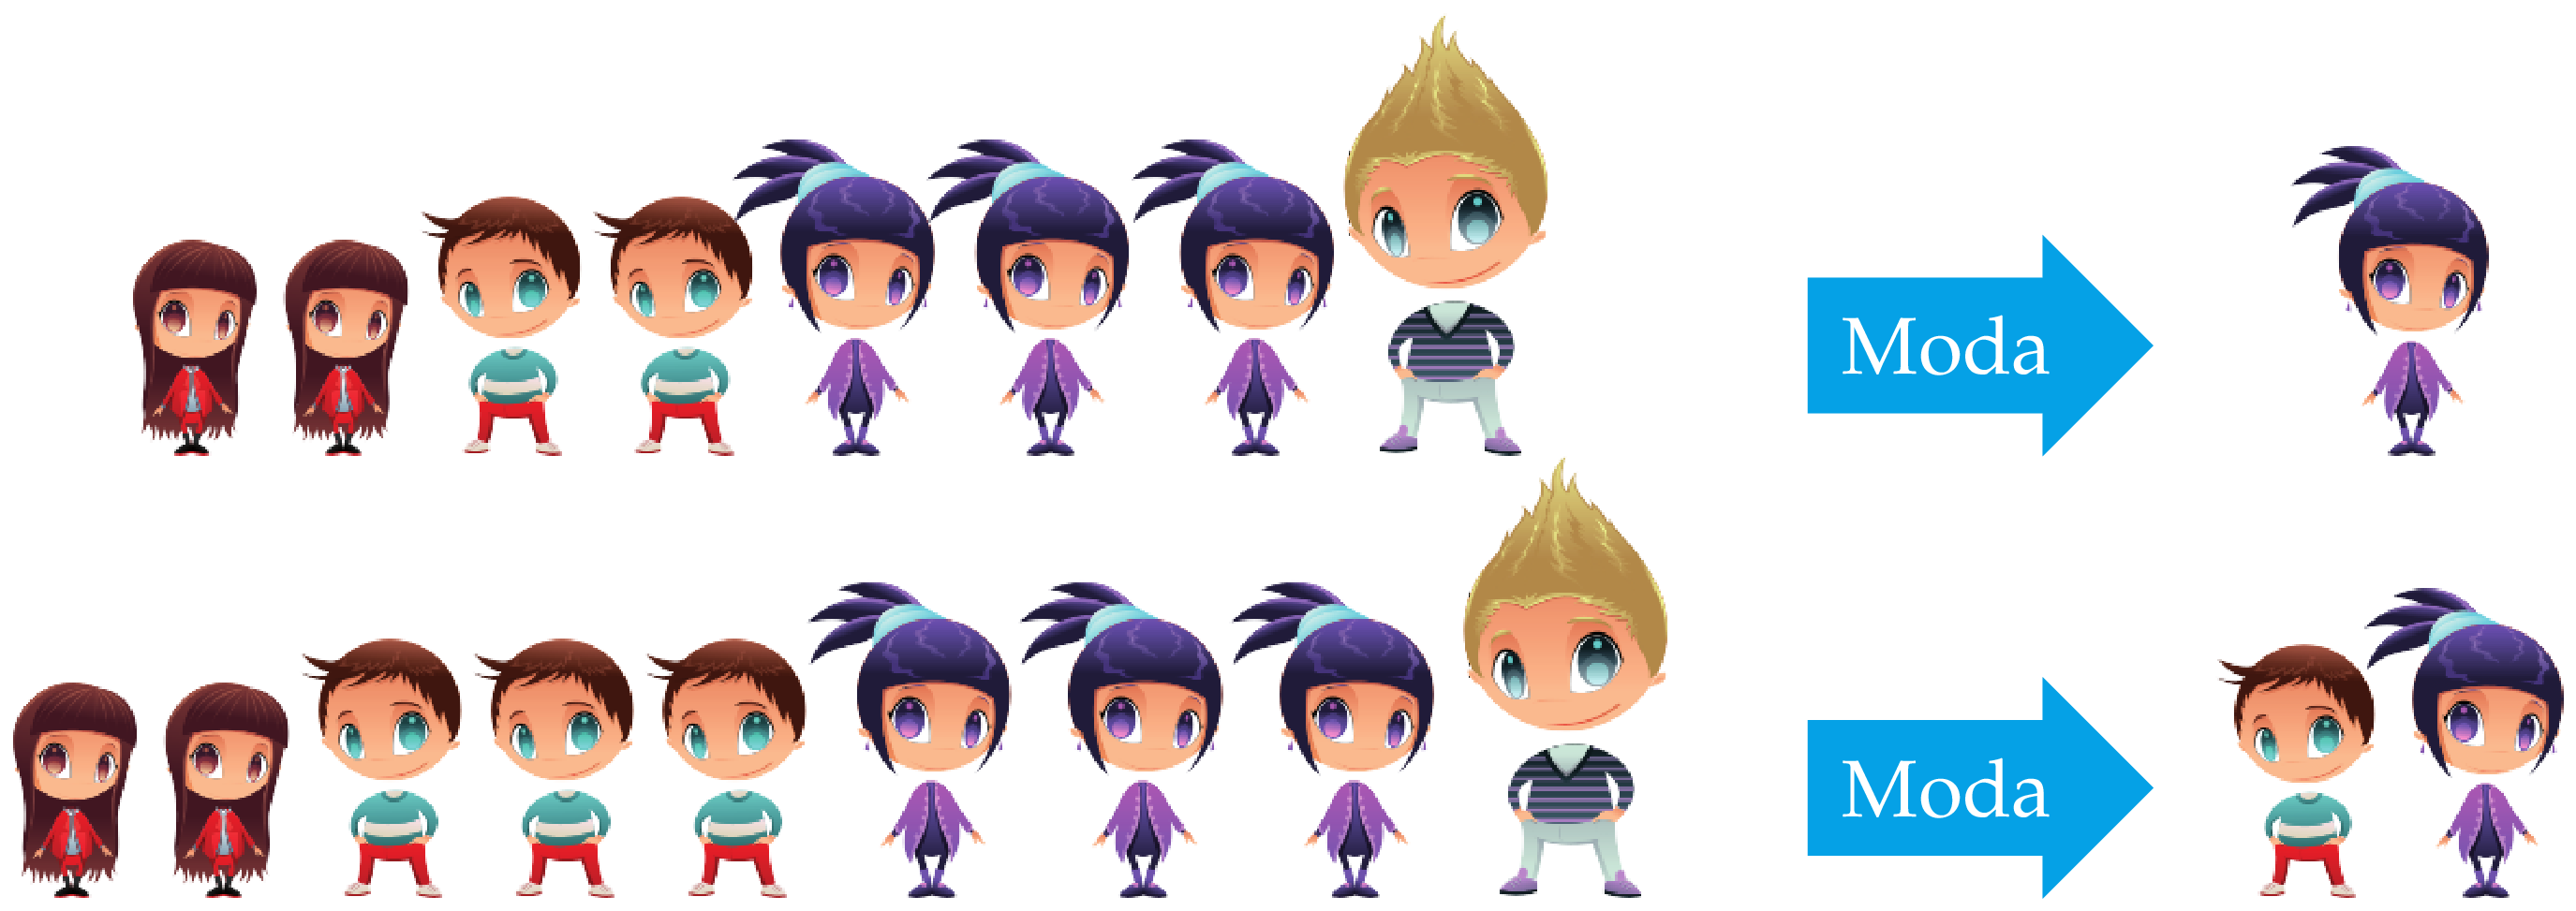
\includegraphics{./img/descriptiva/moda.png}

}

\caption{Cálculo de la moda.}

\end{figure}

\leavevmode\vadjust pre{\hypertarget{exm-moda-datos-no-agrupados}{}}%
\begin{example}[]\label{exm-moda-datos-no-agrupados}

Utilizando los datos de la muestra del número de hijos en las familias,
el valor con mayor frecuencia es 2, y por tanto la moda es \(Mo=2\).

\[
\begin{array}{rr}
\hline
x_i & n_i \\
\hline
0 & 2 \\
1 & 6 \\
\color{red} 2 & 14 \\
3 & 2  \\
4 & 1 \\
\hline
\end{array}
\]

\end{example}

\leavevmode\vadjust pre{\hypertarget{exm-moda-datos-agrupados}{}}%
\begin{example}[]\label{exm-moda-datos-agrupados}

Utilizando los datos de la muestra de estaturas de estudiantes, la clase
con la mayor frecuencia es \((170,180]\), que es la clase modal
\(Mo=(170,180]\).

\[
\begin{array}{cr}
\hline
X & n_i \\
\hline
(150,160] & 2 \\
(160,170] & 8 \\
\color{red}{(170,180]} & 11 \\
(180,190] & 7 \\
(190,200] & 2 \\
\hline
\end{array}
\]

\end{example}

\hypertarget{quuxe9-estaduxedstico-de-tendencia-central-usar}{%
\subsection{¿Qué estadístico de tendencia central
usar?}\label{quuxe9-estaduxedstico-de-tendencia-central-usar}}

En general, siempre que puedan calcularse los estadísticos de tendencia
central, es recomendable utilizarlos como valores representativos en el
siguiente orden:

\begin{enumerate}
\def\labelenumi{\arabic{enumi}.}
\item
  Media. La media utiliza más información que el resto ya que para
  calcularla se tiene en cuenta la magnitud de los datos.
\item
  Mediana. La mediana utiliza menos información que la media, pero más
  que la moda, ya que para calcularla se tiene en cuenta el orden de los
  datos.
\item
  Moda. La moda es la que menos información utiliza ya que para
  calcularla sólo se tienen en cuenta las frecuencias absolutas.
\end{enumerate}

\begin{tcolorbox}[enhanced jigsaw, coltitle=black, breakable, bottomrule=.15mm, colback=white, bottomtitle=1mm, toprule=.15mm, opacitybacktitle=0.6, titlerule=0mm, toptitle=1mm, title=\textcolor{quarto-callout-warning-color}{\faExclamationTriangle}\hspace{0.5em}{Advertencia}, colframe=quarto-callout-warning-color-frame, opacityback=0, arc=.35mm, left=2mm, rightrule=.15mm, leftrule=.75mm, colbacktitle=quarto-callout-warning-color!10!white]

Hay que tener cuidado con los datos atípicos, ya que la media puede
distorsionarse cuando hay datos atípicos. En tal caso es mejor utilizar
la mediana como valor más representativo.

\end{tcolorbox}

\leavevmode\vadjust pre{\hypertarget{exm-media-mediana-datos-atipicos}{}}%
\begin{example}[]\label{exm-media-mediana-datos-atipicos}

Si una muestra de número de hijos de 7 familias es

0, 0, 1, 1, 2, 2, 15,

entonces, \(\bar{x}=3\) hijos y \(Me=1\) hijo.

\emph{¿Qué medida representa mejor el número de hijos en la muestra?}

\end{example}

\hypertarget{medidas-de-posiciuxf3n-no-centrales}{%
\subsection{Medidas de posición no
centrales}\label{medidas-de-posiciuxf3n-no-centrales}}

Las medidas de posición no centrales o \emph{cuantiles} dividen la
distribución en partes iguales.

Los más utilizados son:

\textbf{Cuartiles}: Dividen la distribución en 4 partes iguales. Hay 3
cuartiles: \(C_1\) (25\% acumulado), \(C_2\) (50\% acumulado), \(C_3\)
(75\% acumulado).

\textbf{Deciles}: Dividen la distribución en 10 partes iguales. Hay 9
deciles: \(D_1\) (10\% acumulado),\ldots, \(D_9\) (90\% acumulado).

\textbf{Percentiles}: Dividen la distribución en 100 partes iguales. Hay
99 percentiles: \(P_1\) (1\% acumulado),\ldots, \(P_{99}\) (99\%
acumulado).

\begin{figure}

{\centering 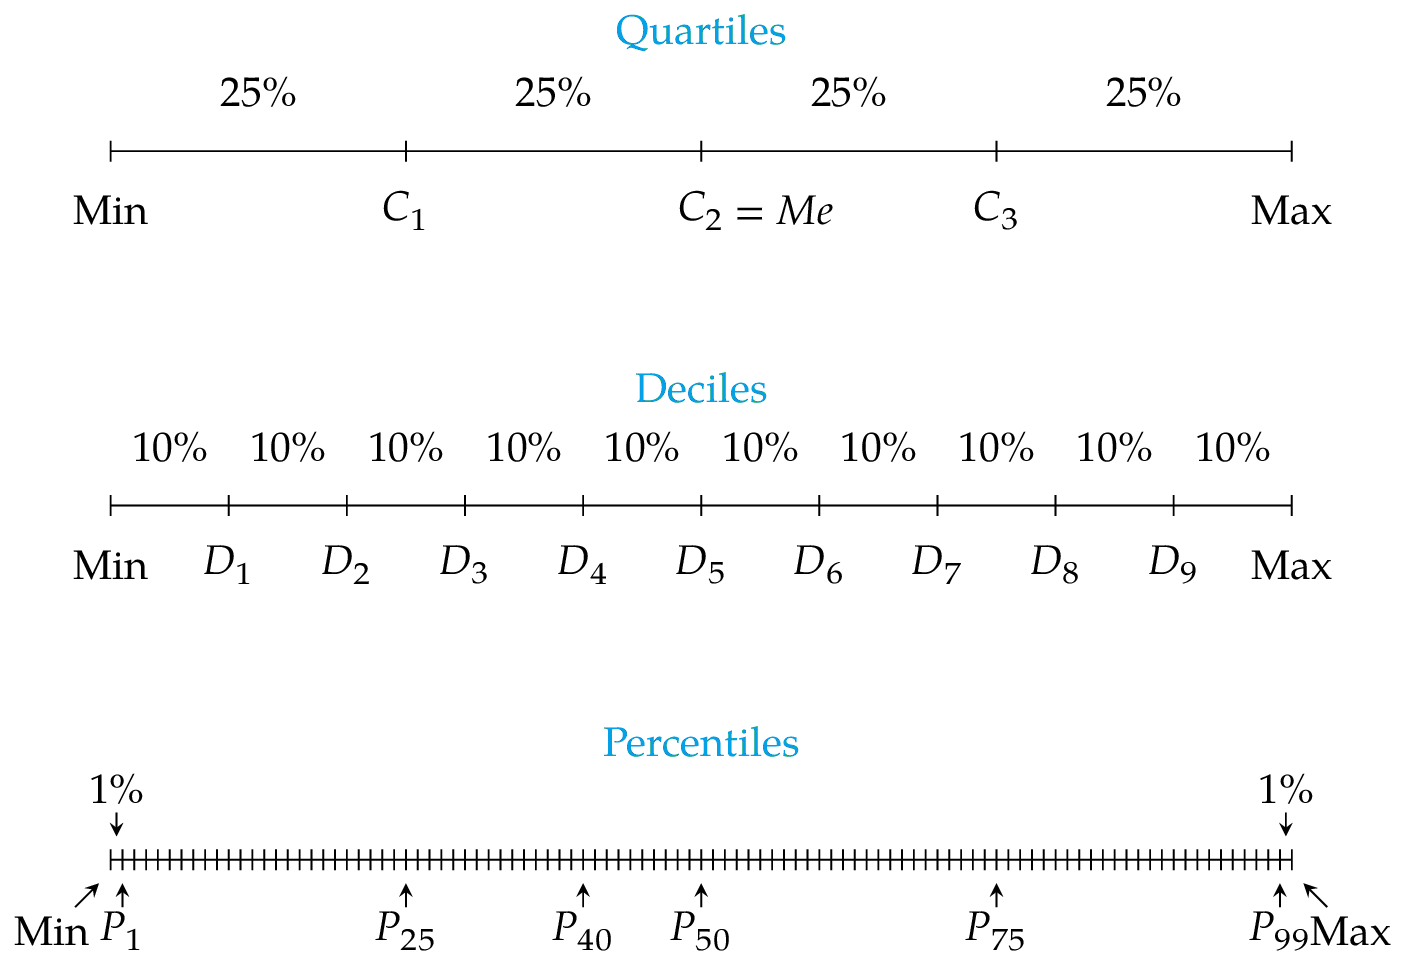
\includegraphics{./img/descriptiva/cuantiles.png}

}

\caption{Cuartiles, deciles y percentiles.}

\end{figure}

Obsérvese que hay una correspondencia entre los cuartiles, los deciles y
los percentiles. Por ejemplo, el primer cuartil coincide con el
percentil 25, y el cuarto decil coincide con el percentil 40.

Los cuantiles se calculan de forma similar a la mediana. La única
diferencia es la frecuencia relativa acumulada que corresponde a cada
cuantil.

\begin{figure}

{\centering 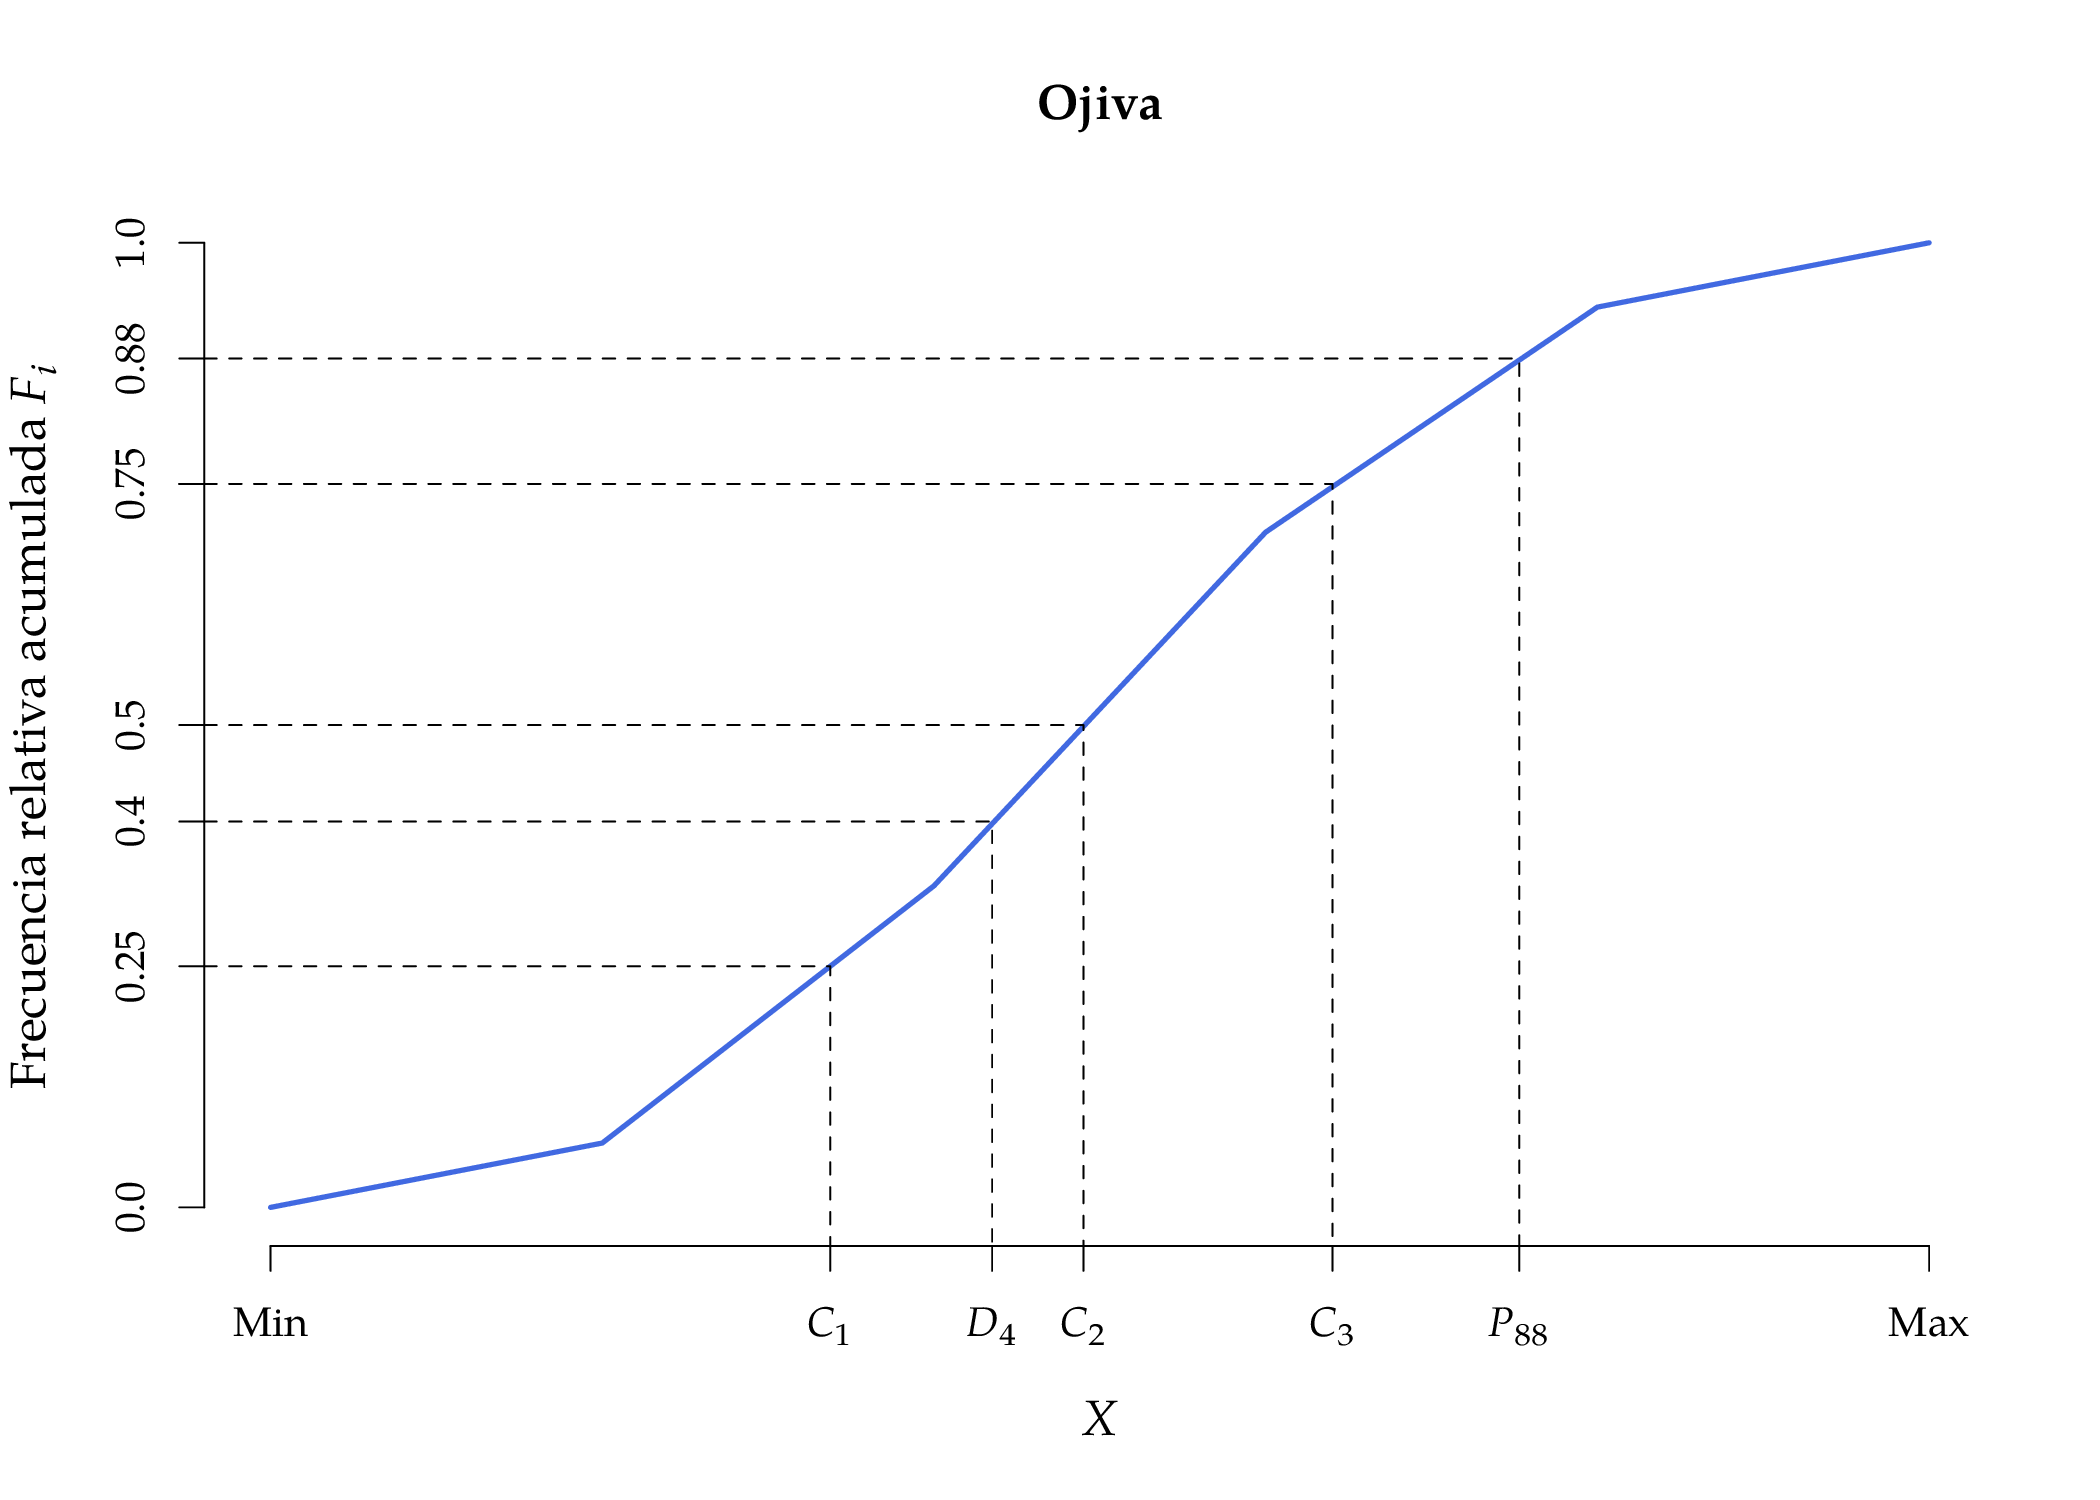
\includegraphics{./img/descriptiva/cuantiles_calculo.png}

}

\caption{Cálculo de cuartiles, deciles y percentiles.}

\end{figure}

\leavevmode\vadjust pre{\hypertarget{exm-cuantiles-datos-no-agrupados}{}}%
\begin{example}[]\label{exm-cuantiles-datos-no-agrupados}

Utilizando los datos de la muestra del número de hijos de las familias,
la frecuencia relativa acumulada era

\[
\begin{array}{rr}
\hline
x_i & F_i \\
\hline
0 & 0.08\\
1 & 0.32\\
2 & 0.88\\
3 & 0.96\\
4 & 1\\
\hline
\end{array}
\]

\begin{align*}
F_{C_1}=0.25 &\Rightarrow Q_1 = 1 \text{ hijos},\\
F_{C_2}=0.5 &\Rightarrow Q_2 = 2 \text{ hijos},\\
F_{C_3}=0.75 &\Rightarrow Q_3 = 2 \text{ hijos},\\
F_{D_4}=0.4 &\Rightarrow D_4 = 2 \text{ hijos},\\
F_{P_{92}}=0.92 &\Rightarrow P_{92} = 3 \text{ hijos}.
\end{align*}

\end{example}

\hypertarget{estaduxedsticos-de-dispersiuxf3n}{%
\section{Estadísticos de
dispersión}\label{estaduxedsticos-de-dispersiuxf3n}}

La \emph{dispersión} se refiere a la heterogeneidad o variabilidad de
los datos. Así pues, los estadísticos de dispersión mide la variabilidad
global de los datos, o con respecto a una medida de tendencia central.

Para las variables cuantitativas, las más empleadas son:

\begin{itemize}
\tightlist
\item
  Recorrido.
\item
  Rango Intercuartílico.
\item
  Varianza.
\item
  Desviación Típica.
\item
  Coeficiente de Variación.
\end{itemize}

\hypertarget{recorrido}{%
\subsection{Recorrido}\label{recorrido}}

\leavevmode\vadjust pre{\hypertarget{def-recorrido-muestral}{}}%
\begin{definition}[Recorrido muestral
\(Re\)]\label{def-recorrido-muestral}

El \emph{recorrido muestral} o \emph{rango muestral} de una variable
\(X\) se define como la diferencia entre el máximo y el mínimo de los
valores en la muestra.

\[Re = \max_{x_i} -\min_{x_i}\]

\end{definition}

\begin{figure}

{\centering 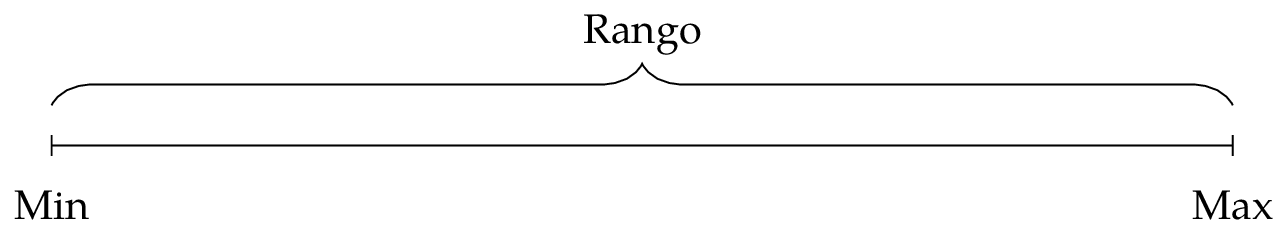
\includegraphics{./img/descriptiva/rango.png}

}

\caption{Rango muestral.}

\end{figure}

El recorrido mide la máxima variación que hay entre los datos
muestrales. No obstante, es muy sensible a datos atípicos ya que suelen
aparecer justo en los extremos de la distribución, por lo que no se
suele utilizar mucho.

\hypertarget{rango-intercuartuxedlico}{%
\subsection{Rango intercuartílico}\label{rango-intercuartuxedlico}}

Para evitar el problema de los datos atípicos en el recorrido, se puede
utilizar el primer y tercer cuartil en lugar del mínimo y el máximo.

\leavevmode\vadjust pre{\hypertarget{def-rango-intercuartilico}{}}%
\begin{definition}[Rango intercuartílico muestral
\(RI\)]\label{def-rango-intercuartilico}

El \emph{rango intercuartílico muestral} de una variable \(X\) se define
como la diferencia entre el tercer y el primer cuartil de la muestra.

\[RI = C_3 -C_1\]

\end{definition}

\begin{figure}

{\centering 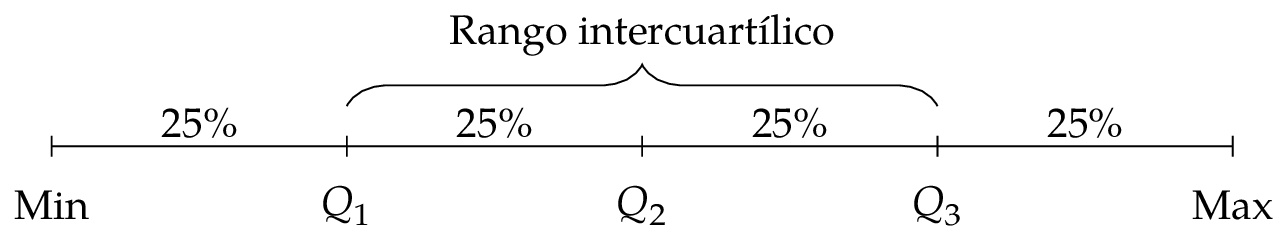
\includegraphics{./img/descriptiva/rango_intercuartilico.png}

}

\caption{Rango intercuartílico.}

\end{figure}

El rango intercuartílico mide la dispersión del 50\% de los datos
centrales.

\hypertarget{diagrama-de-caja-y-bigotes}{%
\subsection{Diagrama de caja y
bigotes}\label{diagrama-de-caja-y-bigotes}}

La dispersión de una variable suele representarse gráficamente mediante
un \emph{diagrama de caja y bigotes}, que representa cinco estadísticos
descriptivos (mínimo, cuartiles y máximo) conocidos como los \emph{cinco
números}. Consiste en una caja, dibujada desde el primer al tercer
cuartil, que representa el rango intercuartílico, y dos segmentos,
conocidos como \emph{bigotes} inferior y superior. A menudo la caja se
divide en dos por la mediana.

Este diagrama es muy útil y se utiliza para muchos propósitos:

\begin{itemize}
\tightlist
\item
  Sirve para medir la dispersión de los datos ya que representa el rango
  y el rango intercuartílico.
\item
  Sirve para detectar datos atípicos, que son los valores que quedan
  fuera del intervalo definido por los bigotes.
\item
  Sirve para medir la simetría de la distribución, comparando la
  longitud de las cajas y de los bigotes por encima y por debajo de la
  mediana.
\end{itemize}

:::\{\#exm-diagrama-caja\} El diagrama siguiente muestra el diagrama de
caja y bigotes del peso de una muestra de recién nacidos.

\begin{figure}

{\centering 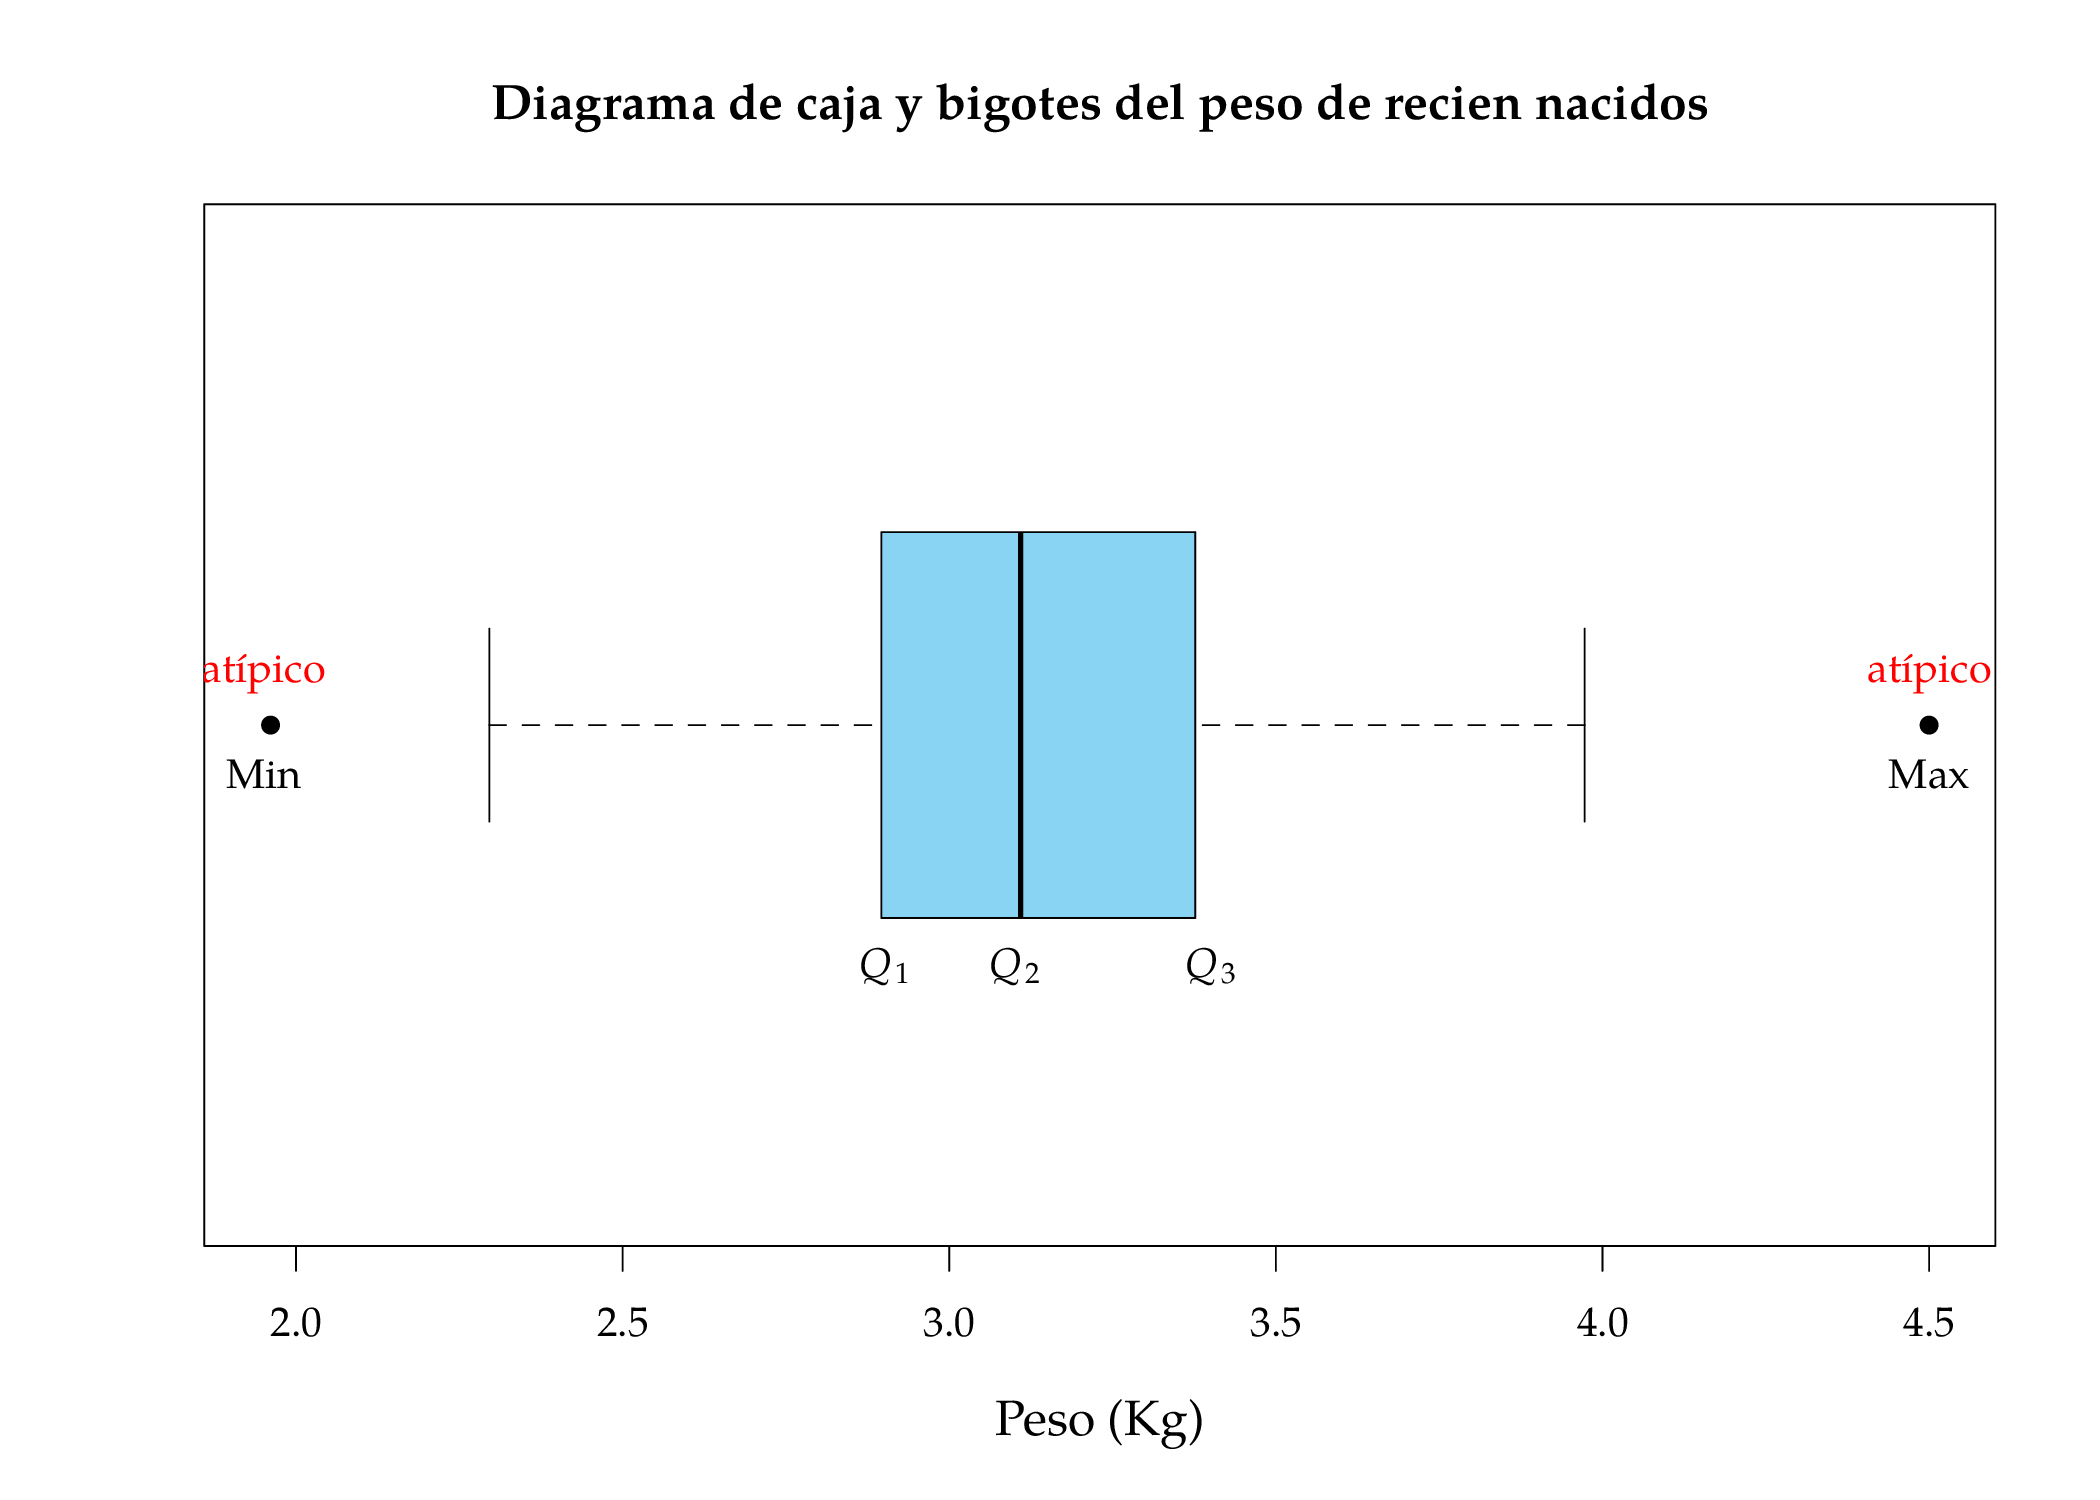
\includegraphics{./img/descriptiva/diagrama_caja.png}

}

\caption{Diagrama de caja y bigotes del peso de recién nacidos.}

\end{figure}

Para construir el diagrama de caja y bigotes hay que seguir los
siguientes pasos:

\begin{enumerate}
\def\labelenumi{\arabic{enumi}.}
\item
  Calcular los cuartiles.
\item
  Dibujar una caja de manera que el extremo inferior caiga sobre el
  primer cuartil y el extremo superior sobre el tercer cuartil.
\item
  Dividir la caja con una línea que caiga sobre el segundo cuartil.
\item
  Para los bigotes inicialmente se calculan dos valores llamados
  \emph{vallas} \(v_1\) y \(v_2\). La valla inferior es el primer
  cuartil menos una vez y media el rango intercuartílico, y la valla
  superior es el tercer cuartil más una vez y media el rango
  intercuartílico.

  \[
   \begin{aligned}
   v_1&=Q_1-1.5\,\text{IQR}\\
   v_2&=Q_3+1.5\,\text{IQR}
   \end{aligned}
   \]

  Las vallas definen el intervalo donde los datos se consideran
  normales. Cualquier valor fuera de ese intervalo se considera un dato
  atípico.\\
  El bigote superior se dibuja desde el borde inferior de la caja hasta
  el menor valor de la muestra que es mayor o igual a la valla inferior,
  y el bigote superior se dibuja desde el borde superior de la caja
  hasta el mayor valor de la muestra que es menor o igual a la valla
  superior.
\end{enumerate}

\begin{tcolorbox}[enhanced jigsaw, coltitle=black, breakable, bottomrule=.15mm, colback=white, bottomtitle=1mm, toprule=.15mm, opacitybacktitle=0.6, titlerule=0mm, toptitle=1mm, title=\textcolor{quarto-callout-warning-color}{\faExclamationTriangle}\hspace{0.5em}{Advertencia}, colframe=quarto-callout-warning-color-frame, opacityback=0, arc=.35mm, left=2mm, rightrule=.15mm, leftrule=.75mm, colbacktitle=quarto-callout-warning-color!10!white]

Los bigotes no son las vallas.

\end{tcolorbox}

\begin{enumerate}
\def\labelenumi{\arabic{enumi}.}
\setcounter{enumi}{4}
\tightlist
\item
  Finalmente, si en la muestra hay algún dato atípico, se dibuja un
  punto para cada uno de ellos.
\end{enumerate}

\leavevmode\vadjust pre{\hypertarget{exm-diagrama-caja}{}}%
\begin{example}[]\label{exm-diagrama-caja}

El diagrama de caja y bigotes de la muestra del número de hijos de las
familias se muestra a continuación.

\begin{figure}

{\centering 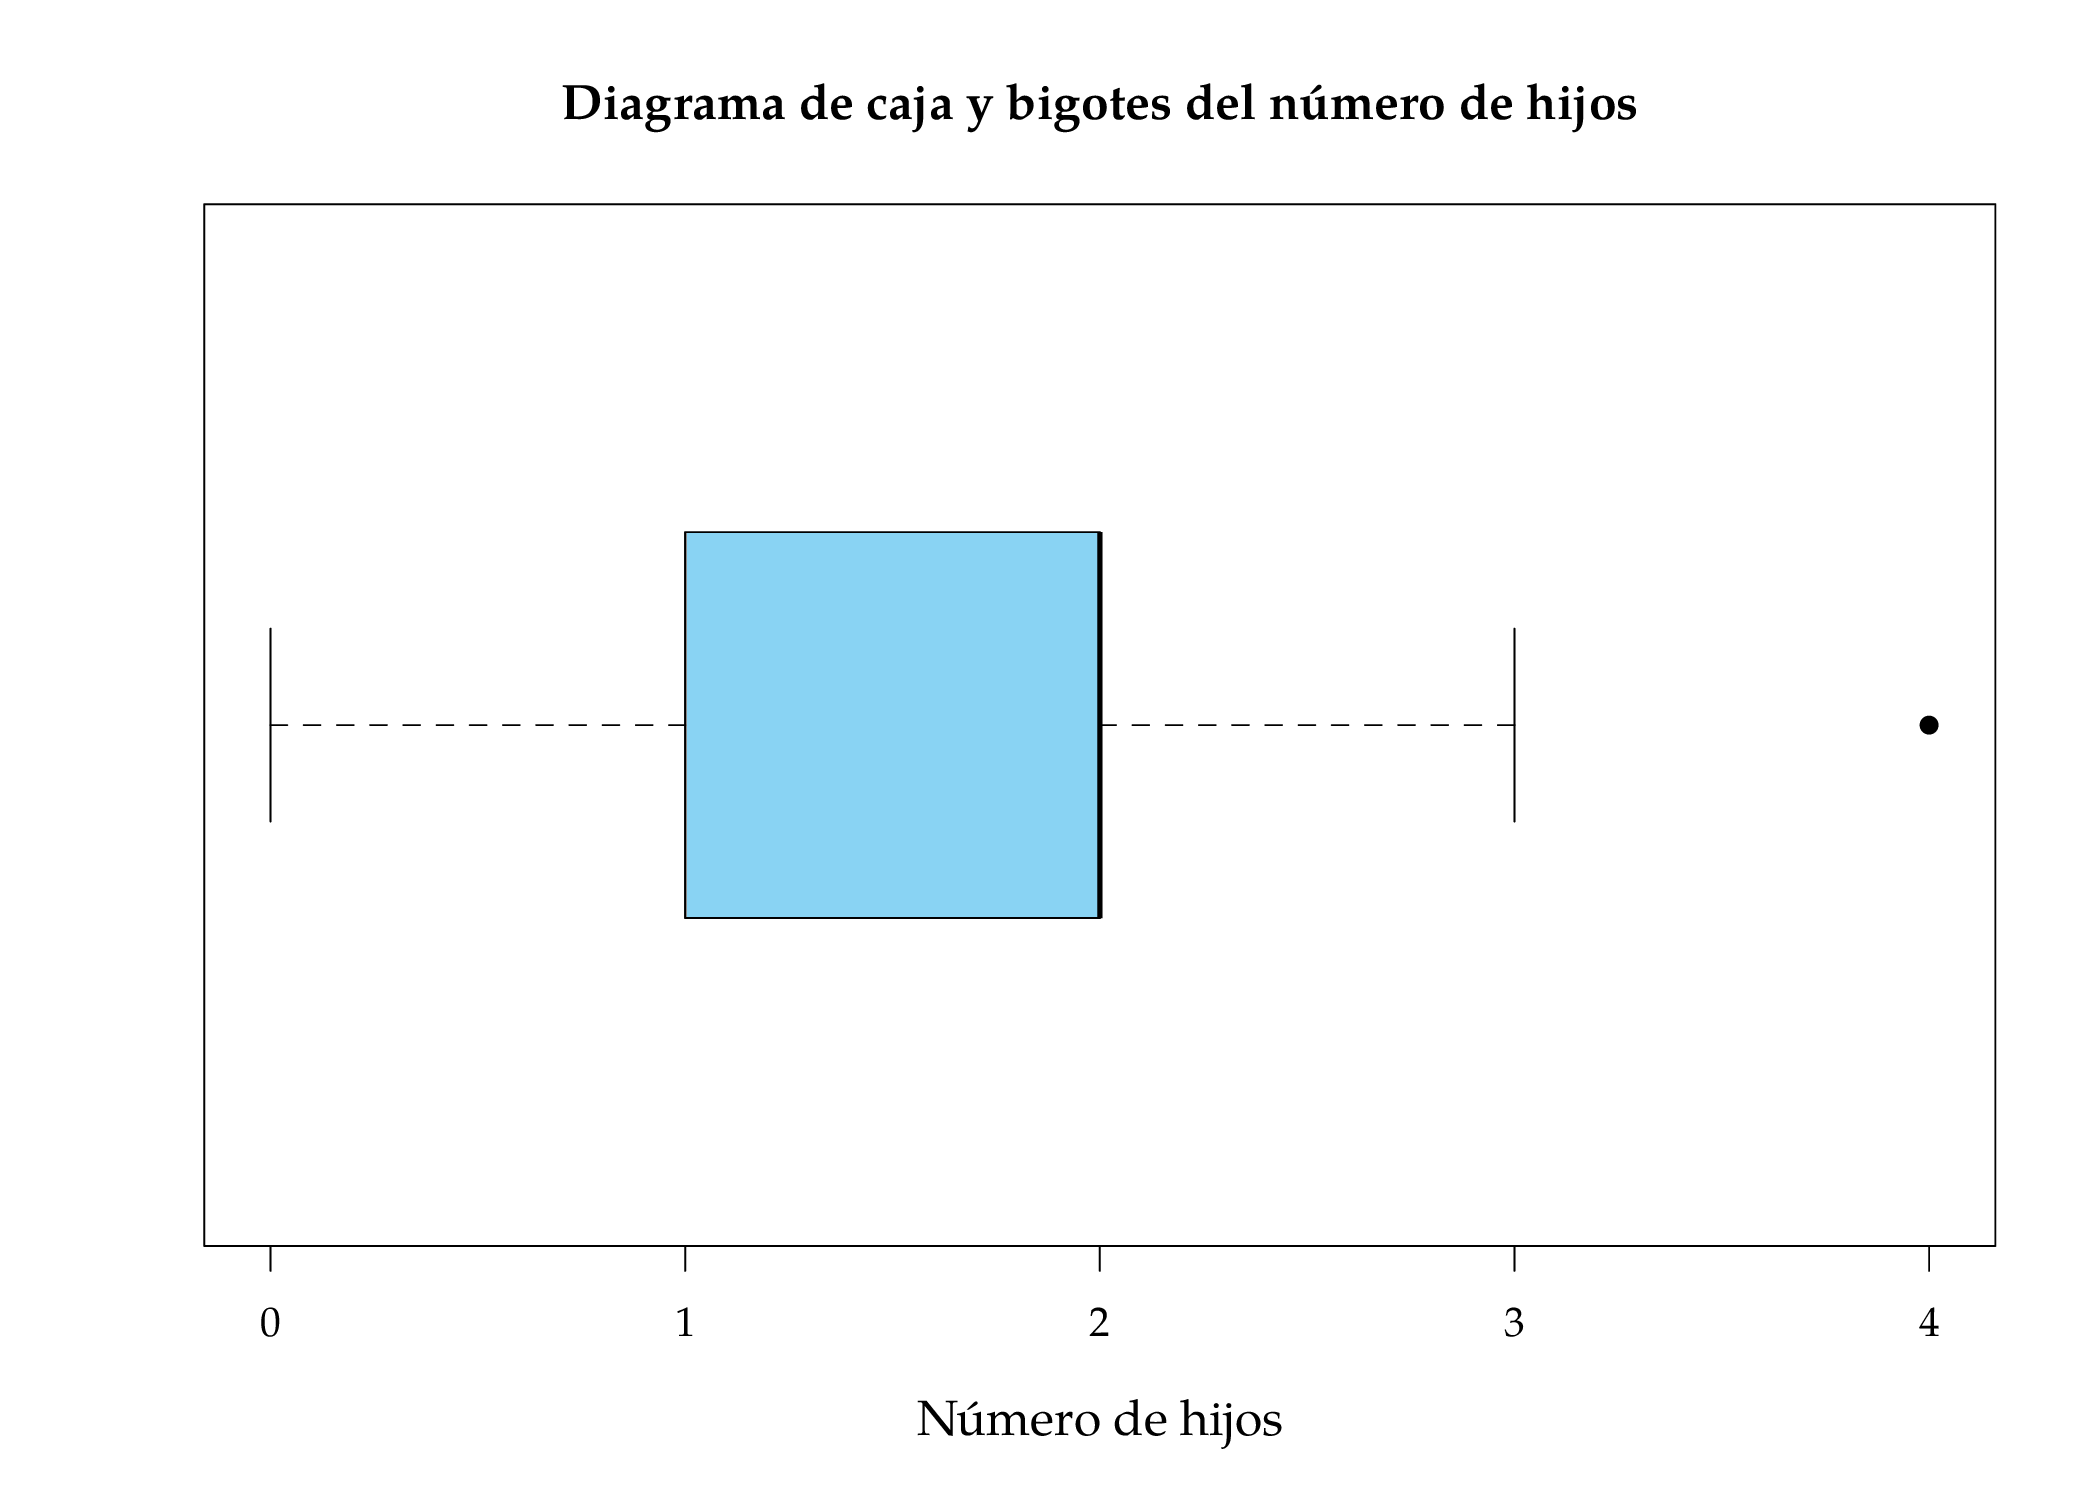
\includegraphics{./img/descriptiva/diagrama_caja_hijos.png}

}

\caption{Diagrama de caja y bigotes del número de hijos.}

\end{figure}

\end{example}

\hypertarget{desviaciones-respecto-de-la-media}{%
\subsubsection{Desviaciones respecto de la
media}\label{desviaciones-respecto-de-la-media}}

Otra forma de medir la variabilidad de una variable es estudiar la
concentración de los valores en torno a algún estadístico de tendencia
central como por ejemplo la media.

Para ello se suele medir la distancia de cada valor a la media. A ese
valor se le llama \textbf{desviación de la media}.

\begin{figure}

{\centering 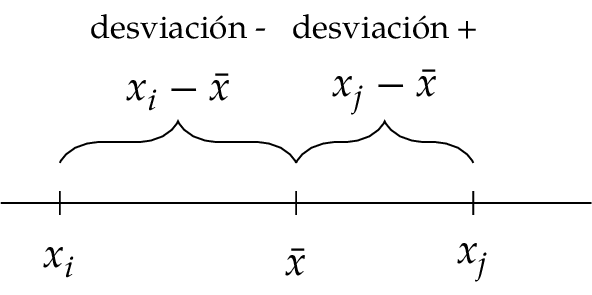
\includegraphics{./img/descriptiva/desviaciones.png}

}

\caption{Desviaciones con respecto a la media.}

\end{figure}

Si las desviaciones son grandes la media no será tan representativa como
cuando la desviaciones sean pequeñas.

\leavevmode\vadjust pre{\hypertarget{exm-desviaciones}{}}%
\begin{example}[]\label{exm-desviaciones}

La siguiente tabla contiene las notas de 3 estudiantes en un curso con
las asignaturas \(A\), \(B\) y \(C\).

\[
\begin{array}{cccc}
\hline
A & B & C & \bar x \\
0 & 5 & 10 & 5 \\
4 & 5 & 6 & 5 \\
5 & 5 & 5 & 5 \\
\hline
\end{array}
\]

Todos los estudiantes tienen la misma media, pero, en qué caso la media
representa mejor el rendimiento en el curso?

\end{example}

\hypertarget{varianza-y-desviaciuxf3n-tuxedpica}{%
\subsection{Varianza y desviación
típica}\label{varianza-y-desviaciuxf3n-tuxedpica}}

\leavevmode\vadjust pre{\hypertarget{def-varianza}{}}%
\begin{definition}[Varianza \(s^2\)]\label{def-varianza}

La \emph{varianza muestral} de una variable \(X\) se define como el
promedio del cuadrado de las desviaciones de los valores de la muestra
respecto de la media muestral.

\[s^2 = \frac{\sum (x_i-\bar x)^2n_i}{n} = \sum (x_i-\bar x)^2f_i\]

\end{definition}

También puede calcularse de manera más sencilla mediante la fórmula

\[s^2 = \frac{\sum x_i^2n_i}{n} -\bar x^2= \sum x_i^2f_i-\bar x^2\]

La varianza tiene las unidades de la variable al cuadrado, por lo que
para facilitar su interpretación se suele utilizar su raíz cuadrada.

\leavevmode\vadjust pre{\hypertarget{def-desviacion-tipica}{}}%
\begin{definition}[Desviación típica \(s\)]\label{def-desviacion-tipica}

La \emph{desviación típica muestral} de una variable \(X\) se define
como la raíz cuadrada positiva de su varianza muestral.

\[s = +\sqrt{s^2}\]

\end{definition}

\begin{tcolorbox}[enhanced jigsaw, coltitle=black, breakable, bottomrule=.15mm, colback=white, bottomtitle=1mm, toprule=.15mm, opacitybacktitle=0.6, titlerule=0mm, toptitle=1mm, title=\textcolor{quarto-callout-tip-color}{\faLightbulb}\hspace{0.5em}{Interpretación}, colframe=quarto-callout-tip-color-frame, opacityback=0, arc=.35mm, left=2mm, rightrule=.15mm, leftrule=.75mm, colbacktitle=quarto-callout-tip-color!10!white]

Tanto la varianza como la desviación típica sirven para cuantificar la
dispersión de los datos en torno a la media. Cuando la varianza o la
desviación típica son pequeñas, los datos de la muestra están
concentrados en torno a la media, y la media es una buena medida de
representatividad. Por contra, cuando la varianza o la desviación típica
son grandes, los datos de la muestra están alejados de la media, y la
media ya no representa tan bien.

\begin{longtable}[]{@{}lcl@{}}
\toprule()
\endhead
Desviación típica pequeña & \(\Rightarrow\) & Media representativa \\
Desviación típica grande & \(\Rightarrow\) & Media no representativa \\
\bottomrule()
\end{longtable}

\end{tcolorbox}

\leavevmode\vadjust pre{\hypertarget{exm-intrepretacion-desviacion-tipica}{}}%
\begin{example}[]\label{exm-intrepretacion-desviacion-tipica}

Las siguientes muestras contienen las notas de dos estudiantes en dos
asignaturas.

\begin{figure}

{\centering 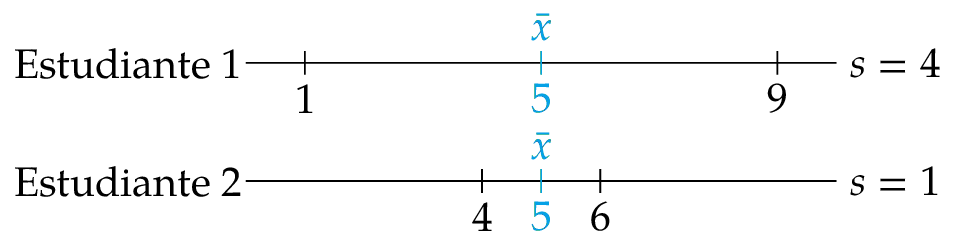
\includegraphics{./img/descriptiva/interpretacion_desviacion_tipica.png}

}

\caption{Interpretación de la desviación típica.}

\end{figure}

\emph{¿Qué media es más representativa?}

\end{example}

\leavevmode\vadjust pre{\hypertarget{exm-desviacion-tipica-datos-no-agrupados}{}}%
\begin{example}[Datos no
agrupados]\label{exm-desviacion-tipica-datos-no-agrupados}

Utilizando los datos de la muestra del número de hijos de las familias,
con una media \(\bar x=1.76\) hijos, y añadiendo una nueva columna a la
tabla de frecuencias con los cuadrados de los valores,

\[
\begin{array}{rrr}
\hline
x_i & n_i & x_i^2n_i \\
\hline
0 & 2 & 0 \\
1 & 6 & 6 \\
2 & 14 & 56\\
3 & 2  & 18\\
4 & 1 & 16 \\
\hline
\sum & 25 & 96 \\
\hline
\end{array}\]

\[s^2 = \frac{\sum x_i^2n_i}{n}-\bar x^2 = \frac{96}{25}-1.76^2= 0.7424 \mbox{ hijos}^2.\]

y la desviación típica es \(s=\sqrt{0.7424} = 0.8616\) hijos.

Comparado este valor con el recorrido, que va de 0 a 4 hijos se observa
que no es demasiado grande por lo que se puede concluir que no hay mucha
dispersión y en consecuencia la media de \(1.76\) hijos representa bien
el número de hijos de las familias de la muestra.

\end{example}

\leavevmode\vadjust pre{\hypertarget{exm-desviacion-tipica-datos-agrupados}{}}%
\begin{example}[Datos
agrupados]\label{exm-desviacion-tipica-datos-agrupados}

Utilizando los datos de la muestra de estaturas de los estudiantes y
agrupando las estaturas en clases, se obtenía una media
\(\bar x = 174.67\) cm. El cálculo de la varianza se realiza igual que
antes pero tomando como valores de la variable las marcas de clase.

\[
\begin{array}{crrr}
\hline
X & x_i & n_i & x_i^2n_i \\
\hline
(150,160] & 155 & 2 & 48050\\
(160,170] & 165 & 8 & 217800\\
(170,180] & 175 & 11 & 336875\\
(180,190] & 185 & 7 & 239575\\
(190,200] & 195 & 2 & 76050\\
\hline
\sum &  & 30 & 918350 \\
\hline
\end{array}
\]

\[s^2 = \frac{\sum x_i^2n_i}{n}-\bar x^2 = \frac{918350}{30}-174.67^2= 102.06 \mbox{ cm}^2,\]

y la desviación típica es \(s=\sqrt{102.06} = 10.1\) cm.

Este valor es bastante pequeño, comparado con el recorrido de la
variable, que va de 150 a 200 cm, por lo que la variable tiene poca
dispersión y en consecuencia su media es muy representativa.

\end{example}

\hypertarget{coeficiente-de-variaciuxf3n}{%
\subsection{Coeficiente de
variación}\label{coeficiente-de-variaciuxf3n}}

Tanto la varianza como la desviación típica tienen unidades y eso
dificulta a veces su interpretación, especialmente cuando se compara la
dispersión de variables con diferentes unidades.

Por este motivo, es también común utilizar la siguiente medida de
dispersión que no tiene unidades.

\leavevmode\vadjust pre{\hypertarget{def-coeficiente-variacion}{}}%
\begin{definition}[Coeficiente de variación muestral
\(cv\)]\label{def-coeficiente-variacion}

El \emph{coeficiente de variación muestral} de una variable \(X\) se
define como el cociente entre su desviación típica muestral y el valor
absoluto de su media muestral.

\[cv = \frac{s}{|\bar x|}\]

\end{definition}

\begin{tcolorbox}[enhanced jigsaw, coltitle=black, breakable, bottomrule=.15mm, colback=white, bottomtitle=1mm, toprule=.15mm, opacitybacktitle=0.6, titlerule=0mm, toptitle=1mm, title=\textcolor{quarto-callout-tip-color}{\faLightbulb}\hspace{0.5em}{Interpretación}, colframe=quarto-callout-tip-color-frame, opacityback=0, arc=.35mm, left=2mm, rightrule=.15mm, leftrule=.75mm, colbacktitle=quarto-callout-tip-color!10!white]

El coeficiente de variación muestral mide la dispersión relativa de los
valores de la muestra en torno a la media muestral.

Como no tiene unidades, es muy sencillo de interpretar: Cuanto mayor
sea, mayor será la dispersión relativa con respecto a la media y menos
representativa será la media.

\end{tcolorbox}

El coeficiente de variación es muy útil para comparar la dispersión de
distribuciones de variables diferentes, incluso si las variables tienen
unidades diferentes.

\leavevmode\vadjust pre{\hypertarget{exm-coeficiente-variacion}{}}%
\begin{example}[]\label{exm-coeficiente-variacion}

En la muestra del número de hijos, donde la media era \(\bar x=1.76\)
hijos y la desviación típica \(s=0.8616\) hijos, el coeficiente de
variación vale

\[cv = \frac{s}{|\bar x|} = \frac{0.8616}{|1.76|} = 0.49.\]

En la muestra de las estaturas, donde la media era \(\bar x=174.67\) cm
y la desviación típica \(s=10.1\) cm, el coeficiente de variación vale

\[cv = \frac{s}{|\bar x|} = \frac{10.1}{|174.67|} = 0.06.\]

Esto significa que la dispersión relativa en la muestra de estaturas es
mucho menor que en la del número de hijos, por lo que la media de las
estaturas será más representativa que la media del número de hijos.

\end{example}

\hypertarget{estaduxedsticos-de-forma}{%
\section{Estadísticos de forma}\label{estaduxedsticos-de-forma}}

Son medidas que describen la forma de la distribución.

Los aspectos más relevantes son:

\textbf{Simetría} Mide la simetría de la distribución de frecuencias en
torno a la media. El estadístico más utilizado es el \emph{Coeficiente
de Asimetría de Fisher}.

\textbf{Apuntamiento} Mide el apuntamiento o el grado de concentración
de valores en torno a la media de la distribución de frecuencias. El
estadístico más utilizado es el \emph{Coeficiente de Apuntamiento o
Curtosis}.

\hypertarget{coeficiente-de-asimetruxeda}{%
\subsection{Coeficiente de
asimetría}\label{coeficiente-de-asimetruxeda}}

\leavevmode\vadjust pre{\hypertarget{def-coeficiente-asimetria}{}}%
\begin{definition}[Coeficiente de asimetría muestral
\(g_1\)]\label{def-coeficiente-asimetria}

El \emph{coeficiente de asimetría muestral} de una variable \(X\) es el
promedio de las desviaciones de los valores de la muestra respecto de la
media muestral, elevadas al cubo, dividido por la desviación típica al
cubo.

\[g_1 = \frac{\sum (x_i-\bar x)^3 n_i/n}{s^3} = \frac{\sum (x_i-\bar x)^3 f_i}{s^3}\]

\end{definition}

\begin{tcolorbox}[enhanced jigsaw, coltitle=black, breakable, bottomrule=.15mm, colback=white, bottomtitle=1mm, toprule=.15mm, opacitybacktitle=0.6, titlerule=0mm, toptitle=1mm, title=\textcolor{quarto-callout-tip-color}{\faLightbulb}\hspace{0.5em}{Interpretación}, colframe=quarto-callout-tip-color-frame, opacityback=0, arc=.35mm, left=2mm, rightrule=.15mm, leftrule=.75mm, colbacktitle=quarto-callout-tip-color!10!white]

Mide el grado de simetría de los valores de la muestra con respecto a la
media muestra, es decir, cuantos valores de la muestra están por encima
o por debajo de la media y cómo de alejados de esta.

\begin{itemize}
\tightlist
\item
  \(g_1=0\) indica que hay el mismo número de valores por encima y por
  debajo de la media e igualmente alejados de ella (simétrica).
\end{itemize}

\begin{figure}[H]

{\centering 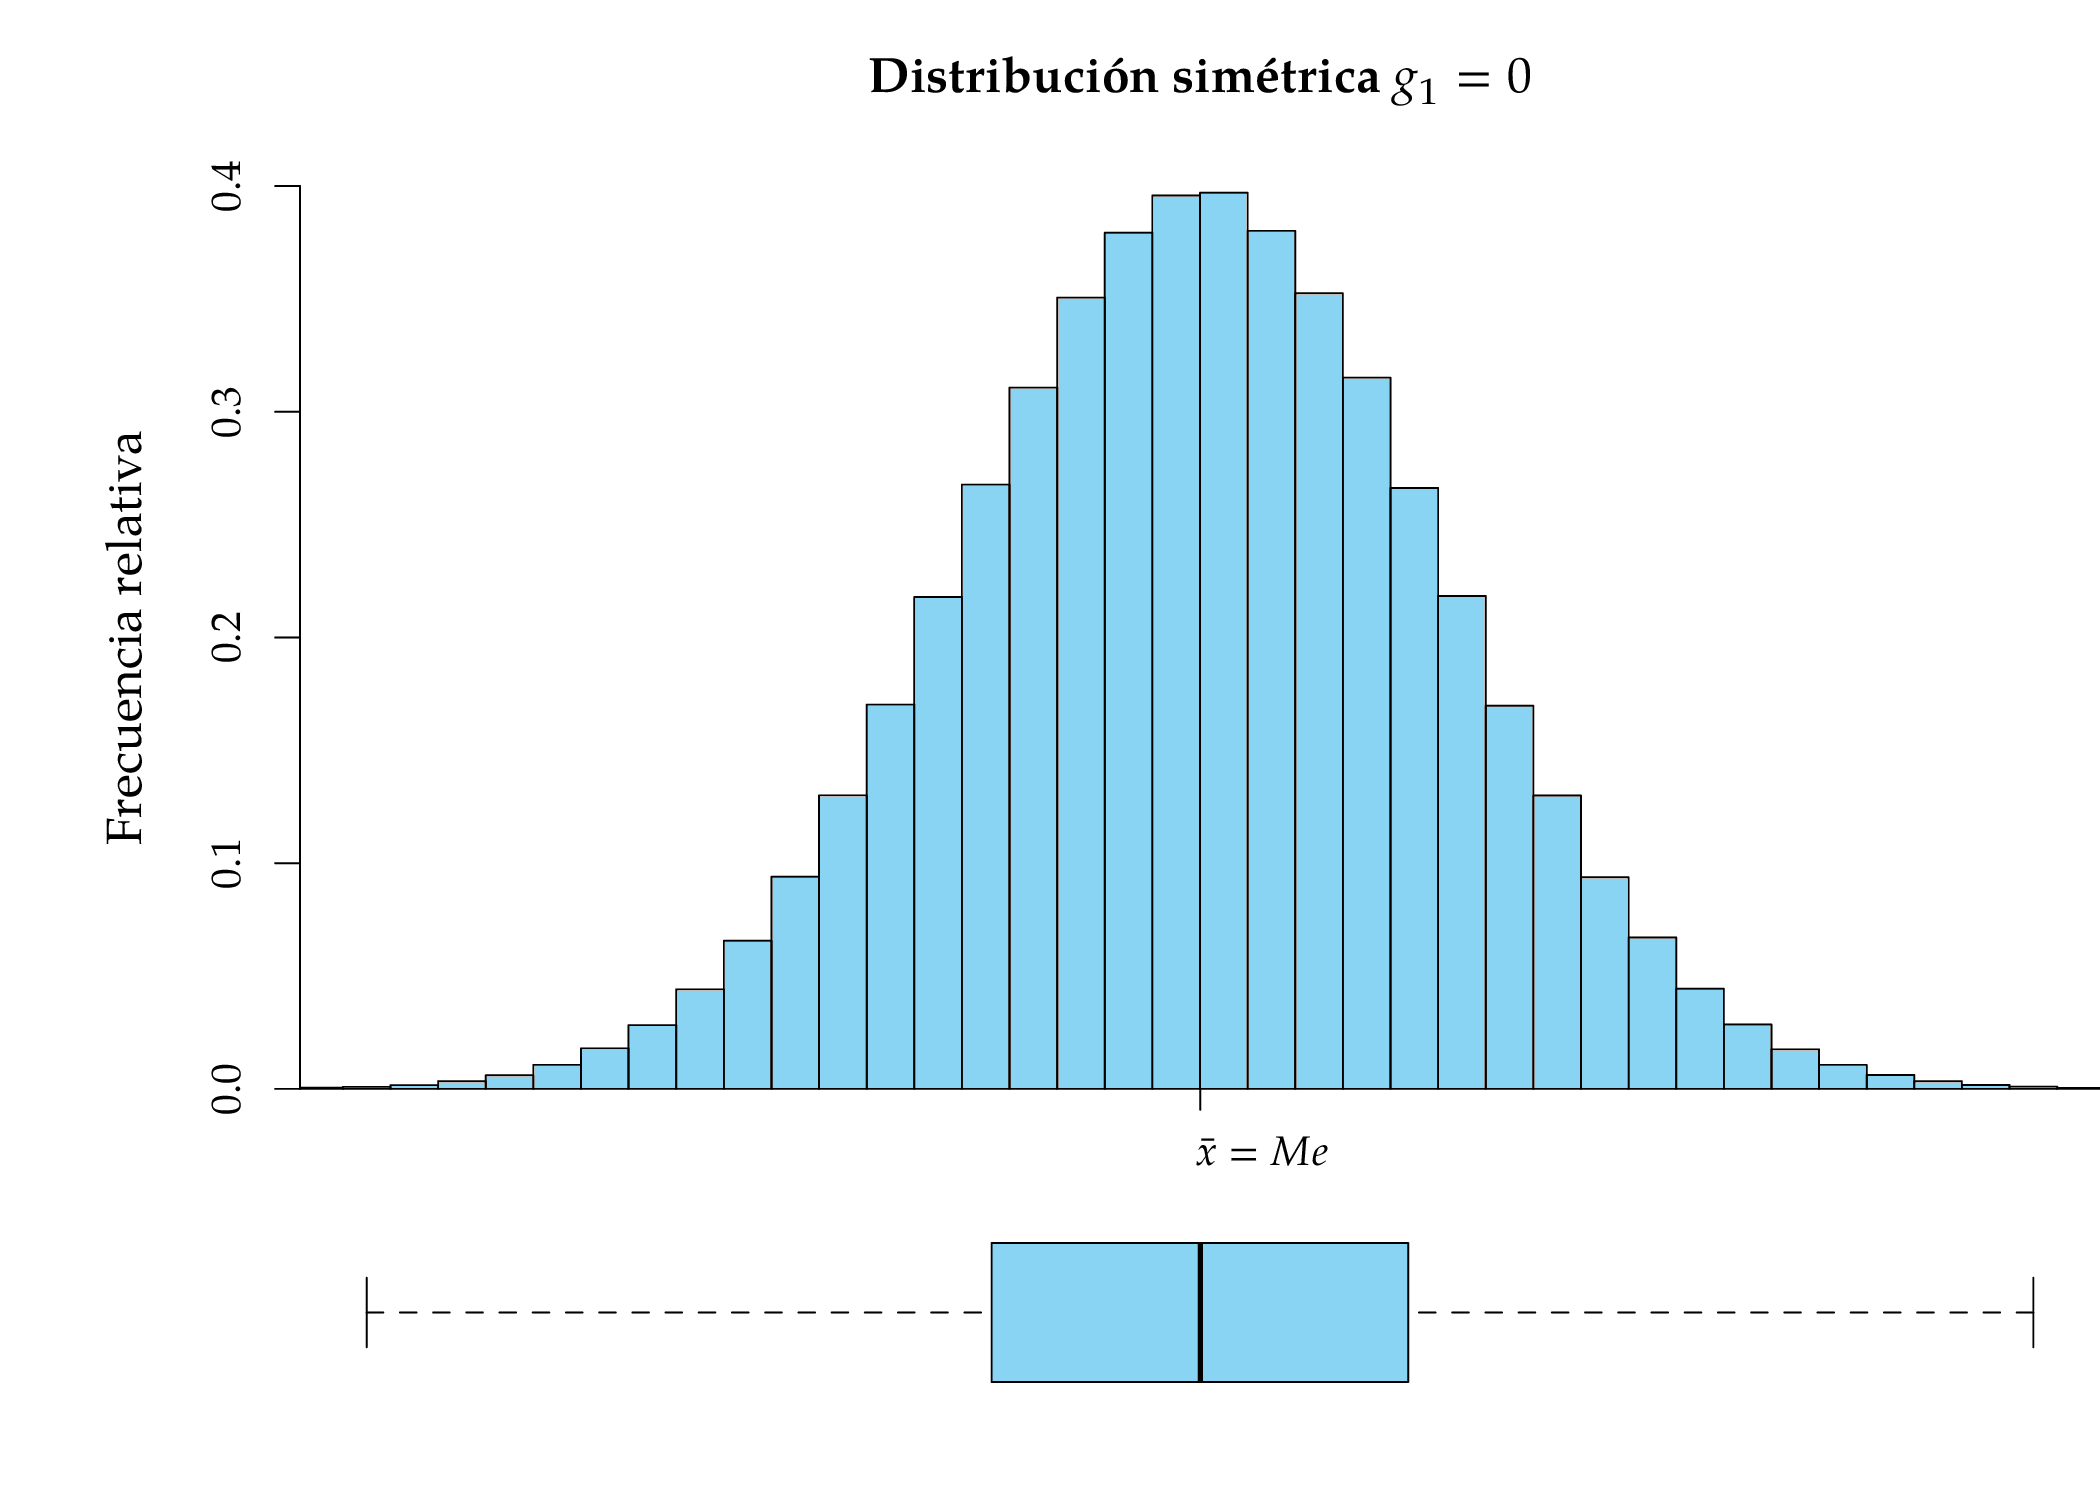
\includegraphics{./img/descriptiva/distribucion_simetrica.png}

}

\caption{Distribución simétrica.}

\end{figure}

\begin{itemize}
\tightlist
\item
  \(g_1<0\) indica que la mayoría de los valores son mayores que la
  media, pero los valores menores están más alejados de ella (asimétrica
  a la izquierda).
\end{itemize}

\begin{figure}[H]

{\centering 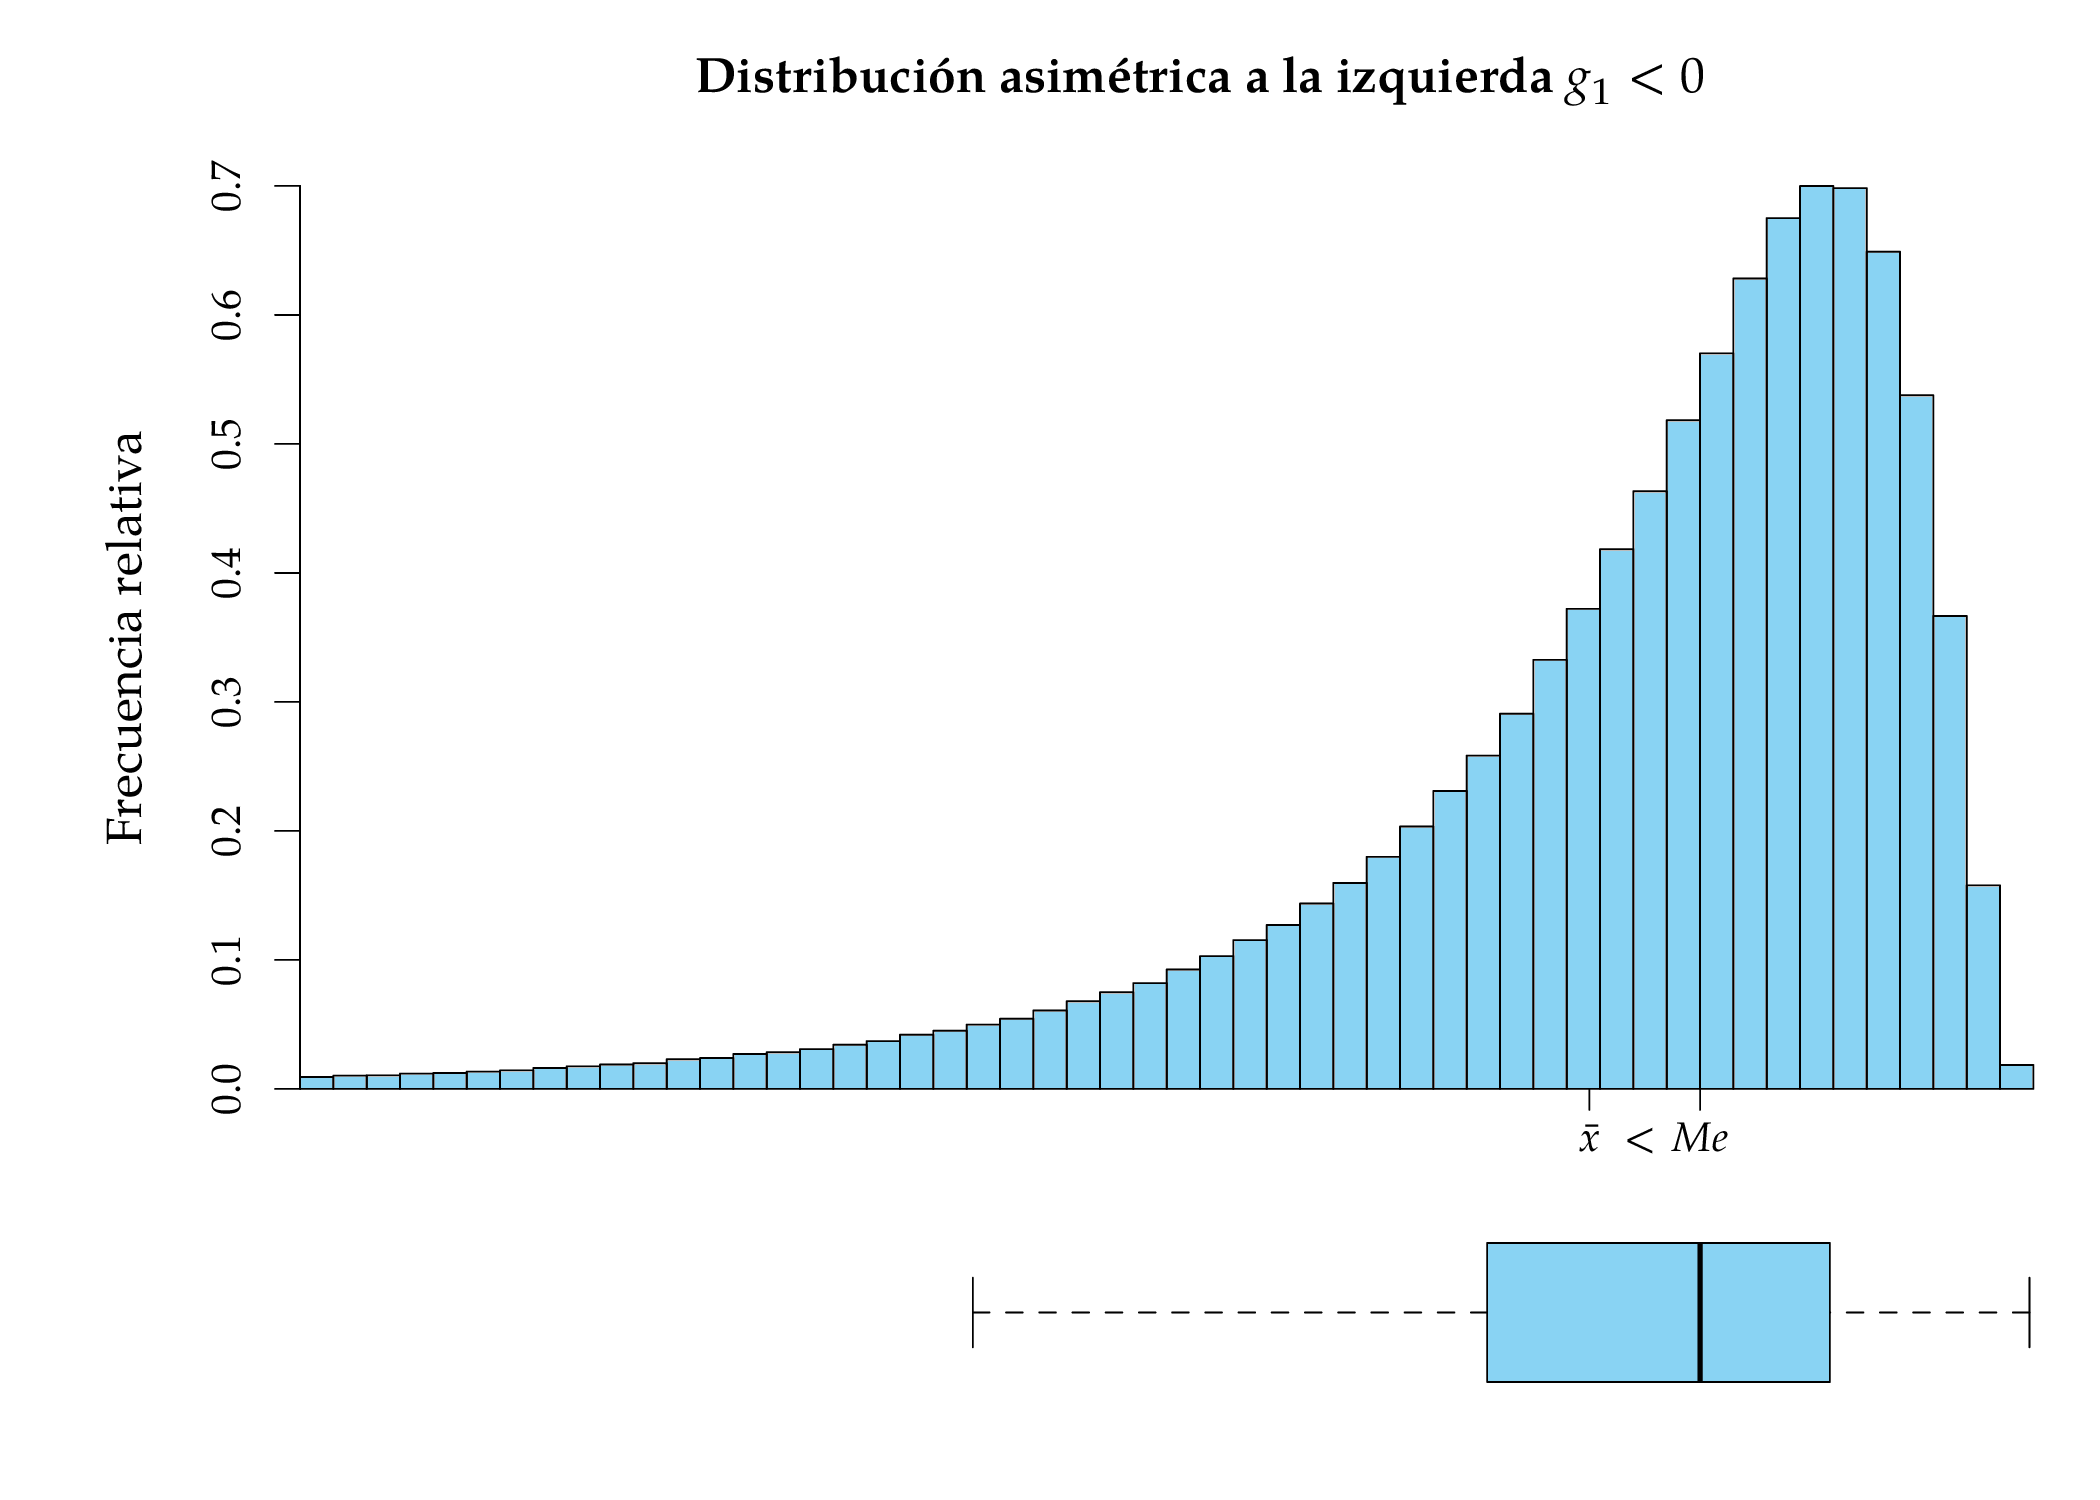
\includegraphics{./img/descriptiva/distribucion_asimetrica_izquierda.png}

}

\caption{Distribución asimétrica hacia la izquierda.}

\end{figure}

\begin{itemize}
\tightlist
\item
  \(g_1>0\) indica que la mayoría de los valores son menores que la
  media, pero los valores mayores están más alejados de ella (asimétrica
  a la derecha).
\end{itemize}

\begin{figure}[H]

{\centering \includegraphics{./img/descriptiva/distribucion_asimetrica_derecha.png}

}

\caption{Distribución asimétrica hacia la derecha.}

\end{figure}

\end{tcolorbox}

\leavevmode\vadjust pre{\hypertarget{exm-coeficiente-asimetria}{}}%
\begin{example}[Datos agrupados]\label{exm-coeficiente-asimetria}

Utilizando la tabla de frecuencias de la muestra de estaturas y
añadiendo una nueva columna con las desviaciones de la media
\(\bar x = 174.67\) cm al cubo, se tiene

\[
\begin{array}{crrrr}
\hline
X & x_i & n_i & x_i-\bar x & (x_i-\bar x)^3 n_i \\
\hline
(150,160] & 155 & 2 & -19.67 & -15221.00\\
(160,170] & 165 & 8 & -9.67 & -7233.85\\
(170,180] & 175 & 11 & 0.33 & 0.40\\
(180,190] & 185 & 7 & 10.33 & 7716.12\\
(190,200] & 195 & 2 & 20.33 & 16805.14\\
\hline
\sum &  & 30 & & 2066.81 \\
\hline
\end{array}
\]

\[g_1 = \frac{\sum (x_i-\bar x)^3n_i/n}{s^3} = \frac{2066.81/30}{10.1^3} = 0.07.\]

Como está cerca de 0, eso significa que la distribución de las estaturas
es casi simétrica.

\end{example}

\hypertarget{coeficiente-de-apuntamiento-o-curtosis}{%
\subsection{Coeficiente de apuntamiento o
curtosis}\label{coeficiente-de-apuntamiento-o-curtosis}}

\leavevmode\vadjust pre{\hypertarget{def-coeficiente-apuntamiento}{}}%
\begin{definition}[Coeficiente de apuntamiento muestral
\(g_2\)]\label{def-coeficiente-apuntamiento}

El \emph{coeficiente de apuntamiento muestral} de una variable \(X\) es
el promedio de las desviaciones de los valores de la muestra respecto de
la media muestral, elevadas a la cuarta, dividido por la desviación
típica a la cuarta y al resultado se le resta 3.

\[g_2 = \frac{\sum (x_i-\bar x)^4 n_i/n}{s^4}-3 = \frac{\sum (x_i-\bar x)^4 f_i}{s^4}-3\]

\end{definition}

\begin{tcolorbox}[enhanced jigsaw, coltitle=black, breakable, bottomrule=.15mm, colback=white, bottomtitle=1mm, toprule=.15mm, opacitybacktitle=0.6, titlerule=0mm, toptitle=1mm, title=\textcolor{quarto-callout-tip-color}{\faLightbulb}\hspace{0.5em}{Interpretación}, colframe=quarto-callout-tip-color-frame, opacityback=0, arc=.35mm, left=2mm, rightrule=.15mm, leftrule=.75mm, colbacktitle=quarto-callout-tip-color!10!white]

El coeficiente de apuntamiento mide la concentración de valores en torno
a la media y la longitud de las colas de la distribución. Se toma como
referencia la distribución normal (campana de Gauss).

\begin{itemize}
\tightlist
\item
  \(g_2=0\) indica que la distribución tienen un apuntamiento normal, es
  decir, la concentración de valores en torno a la media es similar al
  de una campana de Gauss (\emph{mesocúrtica}).
\end{itemize}

\begin{figure}[H]

{\centering \includegraphics{./img/descriptiva/distribucion_mesocurtica.png}

}

\caption{Distribución mesocúrtica.}

\end{figure}

\begin{itemize}
\tightlist
\item
  \(g_2<0\) indica que la distribución tiene menos apuntamiento de lo
  normal, es decir, la concentración de valores en torno a la media es
  menor que en una campana de Gauss (\emph{platicúrtica}).
\end{itemize}

\begin{figure}[H]

{\centering \includegraphics{./img/descriptiva/distribucion_platicurtica.png}

}

\caption{Distribución platicúrtica.}

\end{figure}

\begin{itemize}
\tightlist
\item
  \(g_2>0\) indica que la distribución tiene más apuntamiento de lo
  normal, es decir, la concentración de valores en torno a la media es
  menor que en una campana de Gauss (\emph{leptocúrtica}).
\end{itemize}

\begin{figure}[H]

{\centering \includegraphics{./img/descriptiva/distribucion_leptocurtica.png}

}

\caption{Distribución leptocúrtica.}

\end{figure}

\end{tcolorbox}

:::\{\#exm-coeficiente-apuntamiento\} \#\# Datos agrupados Utilizando la
tabla de frecuencias de la muestra de estaturas y añadiendo una nueva
columna con las desviaciones de la media \(\bar x = 174.67\) cm a la
cuarta, se tiene

\[
\begin{array}{rrrrr}
\hline
X & x_i & n_i & x_i-\bar x & (x_i-\bar x)^4 n_i\\
\hline
(150,160] & 155 & 2 & -19.67 & 299396.99\\
(160,170] & 165 & 8 & -9.67 & 69951.31\\
(170,180] & 175 & 11 & 0.33 & 0.13\\
(180,190] & 185 & 7 & 10.33 & 79707.53\\
(190,200] & 195 & 2 & 20.33 & 341648.49\\
\hline
\sum &  & 30 & & 790704.45 \\
\hline
\end{array}
\]

\[g_2 = \frac{\sum (x_i-\bar x)^4n_i/n}{s^4} - 3 = \frac{790704.45/30}{10.1^4}-3 = -0.47.\]

Como se trata de un valor negativo, aunque cercano a 0, podemos decir
que la distribución es ligeramente platicúrtica.

Como se verá más adelante en la parte de inferencia, muchas de las
pruebas estadísticas solo pueden aplicarse a poblaciones normales.

Las poblaciones normales se caracterizan por ser simétricas y
mesocúrticas, de manera que, tanto el coeficiente de asimetría como el
de apuntamiento pueden utilizarse para contrastar si los datos de la
muestra provienen de una población normal.

\begin{tcolorbox}[enhanced jigsaw, coltitle=black, breakable, bottomrule=.15mm, colback=white, bottomtitle=1mm, toprule=.15mm, opacitybacktitle=0.6, titlerule=0mm, toptitle=1mm, title=\textcolor{quarto-callout-tip-color}{\faLightbulb}\hspace{0.5em}{Interpretación}, colframe=quarto-callout-tip-color-frame, opacityback=0, arc=.35mm, left=2mm, rightrule=.15mm, leftrule=.75mm, colbacktitle=quarto-callout-tip-color!10!white]

En general, se suele rechazar la hipótesis de normalidad de la población
cuando \(g_1\) o \(g_2\) estén fuera del intervalo \([-2,2]\).

\end{tcolorbox}

En tal caso, lo habitual es aplicar alguna transformación a la variable
para corregir la anormalidad.

\hypertarget{distribuciones-no-normales}{%
\subsection{Distribuciones no
normales}\label{distribuciones-no-normales}}

\hypertarget{distribuciuxf3n-asimuxe9trica-a-la-derecha-no-normal}{%
\subsubsection{Distribución asimétrica a la derecha no
normal}\label{distribuciuxf3n-asimuxe9trica-a-la-derecha-no-normal}}

Un ejemplo de distribución asimétrica a la derecha es el ingreso de las
familias.

\begin{figure}

{\centering \includegraphics{./img/descriptiva/ejemplo_distribucion_asimetrica_derecha.png}

}

\caption{Distribucion de los ingresos familiares de EEUU.}

\end{figure}

\hypertarget{distribuciuxf3n-asimuxe9trica-a-la-izquierda-no-normal}{%
\subsubsection{Distribución asimétrica a la izquierda no
normal}\label{distribuciuxf3n-asimuxe9trica-a-la-izquierda-no-normal}}

Un ejemplo de distribución asimétrica a la izquierda es la edad de
fallecimiento.

\begin{figure}

{\centering \includegraphics{./img/descriptiva/ejemplo_distribucion_asimetrica_izquierda.png}

}

\caption{Distribucion de la edad de fallecimiento.}

\end{figure}

\hypertarget{distribuciuxf3n-bimodal-no-normal}{%
\subsubsection{Distribución bimodal no
normal}\label{distribuciuxf3n-bimodal-no-normal}}

Un ejemplo de distribución bimodal es la hora de llegada de los clientes
de un restaurante.

\begin{figure}

{\centering \includegraphics{./img/descriptiva/ejemplo_distribucion_bimodal.png}

}

\caption{Distribucion de la hora de llegada de los clientes de un
restaurante.}

\end{figure}

\hypertarget{transformaciones-de-variables}{%
\section{Transformaciones de
variables}\label{transformaciones-de-variables}}

En muchas ocasiones se suelen transformar los datos brutos para corregir
alguna anormalidad de la distribución o simplemente para trabajar con
unas unidades más cómodas.

Por ejemplo, si estamos trabajando con estaturas medidas en metros y
tenemos los siguientes valores:

\[
1.75 \mbox{ m}, 1.65 \mbox{ m}, 1.80 \mbox{ m},
\]

podemos evitar los decimales multiplicando por 100, es decir, pasando de
metros a centímetros:

\[
175 \mbox{ cm}, 165 \mbox{ cm}, 180 \mbox{ cm},
\]

Y si queremos reducir la magnitud de los datos podemos restarles a todos
el menor de ellos, en este caso, 165cm:

\[10\mbox{cm}, 0\mbox{cm}, 15\mbox{cm},\]

Está claro que este conjunto de datos es mucho más sencillo que el
original. En el fondo lo que se ha hecho es aplicar a los datos la
transformación:

\[Y= 100X-165\]

\hypertarget{transformaciones-lineales}{%
\subsection{Transformaciones lineales}\label{transformaciones-lineales}}

Una de las transformaciones más habituales es la \emph{transformación
lineal}:

\[Y=a+bX.\]

\leavevmode\vadjust pre{\hypertarget{thm-transformaciones-lineales}{}}%
\begin{theorem}[]\label{thm-transformaciones-lineales}

Dada una variable muestral \(X\), si \(Y\) es la variable muestral que
resulta de aplicar a \(X\) la transformación lineal \(Y=a+bX\), entonces

\begin{align*}
\bar y &= a+ b\bar x,\\
s_{y} &= |b|s_{x}
\end{align*}

Además, el coeficiente de curtosis no se altera y el de asimetría sólo
cambia de signo si \(b\) es negativo.

\end{theorem}

\begin{tcolorbox}[enhanced jigsaw, coltitle=black, breakable, bottomrule=.15mm, colback=white, bottomtitle=1mm, toprule=.15mm, opacitybacktitle=0.6, titlerule=0mm, toptitle=1mm, title=\textcolor{quarto-callout-note-color}{\faInfo}\hspace{0.5em}{Demostración}, colframe=quarto-callout-note-color-frame, opacityback=0, arc=.35mm, left=2mm, rightrule=.15mm, leftrule=.75mm, colbacktitle=quarto-callout-note-color!10!white]

Se deja como ejercicio.

\end{tcolorbox}

\hypertarget{transformaciuxf3n-de-tipificaciuxf3n-y-puntuaciones-tuxedpicas}{%
\subsection{Transformación de tipificación y puntuaciones
típicas}\label{transformaciuxf3n-de-tipificaciuxf3n-y-puntuaciones-tuxedpicas}}

Una de las transformaciones lineales más habituales es la
\emph{tipificación}:

\leavevmode\vadjust pre{\hypertarget{def-variable-tipificada}{}}%
\begin{definition}[Variable tipificada]\label{def-variable-tipificada}

La \emph{variable tipificada} de una variable estadística \(X\) es la
variable que resulta de restarle su media y dividir por su desviación
típica.

\[Z=\frac{X-\bar x}{s_{x}}\]

Para cada valor \(x_i\) de la muestra, la \emph{puntuación típica} es el
valor que resulta de aplicarle la transformación de tipificación

\[z_i=\frac{x_i-\bar x}{s_{x}}.\]

\end{definition}

\begin{tcolorbox}[enhanced jigsaw, coltitle=black, breakable, bottomrule=.15mm, colback=white, bottomtitle=1mm, toprule=.15mm, opacitybacktitle=0.6, titlerule=0mm, toptitle=1mm, title=\textcolor{quarto-callout-tip-color}{\faLightbulb}\hspace{0.5em}{Interpretación}, colframe=quarto-callout-tip-color-frame, opacityback=0, arc=.35mm, left=2mm, rightrule=.15mm, leftrule=.75mm, colbacktitle=quarto-callout-tip-color!10!white]

La puntuación típica es el número de desviaciones típicas que un valor
está por encima o por debajo de la media, y es útil para evitar la
dependencia de una variable respecto de las unidades de medida
empleadas. Esto es útil, por ejemplo, para comparar valores de variables
o muestras distintas.

\end{tcolorbox}

Dada una variable muetral \(X\), si \(Z\) es la variable tipificada de
\(X\), entonces

\[\bar z = 0 \qquad s_{z} = 1.\]

\begin{tcolorbox}[enhanced jigsaw, coltitle=black, breakable, bottomrule=.15mm, colback=white, bottomtitle=1mm, toprule=.15mm, opacitybacktitle=0.6, titlerule=0mm, toptitle=1mm, title=\textcolor{quarto-callout-note-color}{\faInfo}\hspace{0.5em}{Demostración}, colframe=quarto-callout-note-color-frame, opacityback=0, arc=.35mm, left=2mm, rightrule=.15mm, leftrule=.75mm, colbacktitle=quarto-callout-note-color!10!white]

Se deja como ejercicio.

\end{tcolorbox}

\leavevmode\vadjust pre{\hypertarget{exm-tipificacion}{}}%
\begin{example}[]\label{exm-tipificacion}

Las notas de 5 alumnos en dos asignaturas \(X\) e \(Y\) son

\[
\begin{array}{rccccccccc}
\mbox{Alumno:} & 1 & 2 & 3 & 4 & 5\\
\hline
X: & 2 & 5 & 4 & \color{red} 8 & 6 & \qquad & \bar x = 5 & \quad s_x = 2\\
Y: & 1 & 9 & \color{red} 8 & 5 & 2 & \qquad & \bar y = 5 & \quad s_y = 3.16\\
\hline
\end{array}
\]

\emph{¿Ha tenido el mismo rendimiento el cuarto alumno en la asignatura
\(X\) que el tercero en la asignatura \(Y\)?}

Podría parecer que ambos alumnos han tenido el mismo rendimiento puesto
que tienen la misma nota, pero si queremos ver el rendimiento relativo
al resto del grupo, tendríamos que tener en cuenta la dispersión de cada
muestra y medir sus puntuaciones típicas:

\[
\begin{array}{cccccc}
\mbox{Alumno:} & 1 & 2 & 3 & 4 & 5\\
\hline
X: & -1.50 & 0.00 & -0.50 & \color{red}{1.50} & 0.50 \\
Y: & -1.26 & 1.26 & \color{red}{0.95} & 0.00 & -0.95\\
\hline
\end{array}
\]

Es decir, el alumno que tiene un 8 en \(X\) está \(1.5\) veces la
desviación típica por encima de la media de \(X\), mientras que el
alumno que tiene un 8 en \(Y\) sólo está \(0.95\) desviaciones típicas
por encima de la media de \(Y\). Así pues, el primer alumno tuvo un
rendimiento superior al segundo.

Siguiendo con el ejemplo anterior y considerando ambas asignaturas,
\emph{¿cuál es el mejor alumno?}

Si simplemente se suman las puntuaciones de cada asignatura se tiene:

\[\begin{array}{rccccc}
\mbox{Alumno:} & 1 & 2 & 3 & 4 & 5\\
\hline
X: & 2 & 5 & 4 & 8 & 6 \\
Y: & 1 & 9 & 8 & 5 & 2 \\
\hline
\sum & 3 & \color{red}{14} & 12 & 13 & 8
\end{array}
\]

El mejor alumno sería el segundo.

Pero si se considera el rendimiento relativo tomando las puntuaciones
típicas se tiene

\[
\begin{array}{rccccc}
\mbox{Alumno:} & 1 & 2 & 3 & 4 & 5\\
\hline
X: & -1.50 & 0.00 & -0.50 & 1.50 & 0.50 \\
Y: & -1.26 & 1.26 & 0.95 & 0.00 & -0.95\\
\hline
\sum & -2.76 & 1.26 & 0.45 & \color{red}{1.5} & -0.45
\end{array}
\]

Y el mejor alumno sería el cuarto.

\end{example}

\hypertarget{transformaciones-no-lineales}{%
\subsubsection{Transformaciones no
lineales}\label{transformaciones-no-lineales}}

Las transformaciones no lineales son también habituales para corregir la
anormalidad de las distribuciones.

La transformación \(Y=X^2\) comprime la escala para valores pequeños y
la expande para valores altos, de manera que es muy útil para corregir
asimetrías hacia la izquierda.

\begin{figure}

{\centering \includegraphics{./img/descriptiva/transformacion_cuadratica.png}

}

\caption{Transformación cuadrática.}

\end{figure}

Las transformaciones \(Y=\sqrt x\), \(Y= \log X\) y \(Y=1/X\) comprimen
la escala para valores altos y la expanden para valores pequeños, de
manera que son útiles para corregir asimetrías hacia la derecha.

\begin{figure}

{\centering \includegraphics{./img/descriptiva/transformacion_logaritmica.png}

}

\caption{Transformación logarítmica.}

\end{figure}

\hypertarget{variables-clasificadoras-o-factores}{%
\subsection{Variables clasificadoras o
factores}\label{variables-clasificadoras-o-factores}}

En ocasiones interesa describir el comportamiento de una variable, no
para toda la muestra, sino para distintos grupos de individuos
correspondientes a las categorías de otra variable conocida como
\textbf{variable clasificadora} o \textbf{factor}.

\leavevmode\vadjust pre{\hypertarget{exm-factores}{}}%
\begin{example}[]\label{exm-factores}

Dividiendo la muestra de estaturas según el sexo se obtienen dos
submuestras:

\[
\begin{array}{lll}
\hline
\mbox{Mujeres} & & 173, 158, 174, 166, 162, 177, 165, 154, 166, 182, 169, 172, 170, 168. \\
\mbox{Hombres} & & 179, 181, 172, 194, 185, 187, 198, 178, 188, 171, 175, 167, 186, 172, 176, 187. \\
\hline
\end{array}
\]

\end{example}

Habitualmente los factores se usan para comparar la distribución de la
variable principal para cada categoría del factor.

\leavevmode\vadjust pre{\hypertarget{exm-diagramas-agrupados-factores}{}}%
\begin{example}[]\label{exm-diagramas-agrupados-factores}

Los siguientes diagramas permiten comparar la distribución de estaturas
según el sexo.

\begin{figure}

{\centering \includegraphics{./img/descriptiva/histograma_estatura_sexo.png}

}

\caption{Histograma de estaturas por sexo.}

\end{figure}

\begin{figure}

{\centering \includegraphics{./img/descriptiva/diagrama_caja_estatura_sexo.png}

}

\caption{Diagramas de cajas de estaturas por sexo.}

\end{figure}

\end{example}



\end{document}
